%slide 7 - cancel out - contasin out line of theoires - whihc?? - muon pature
\documentclass[12pt,a4paper]{report}

%\usepackage{fancyhdr}

%\pagestyle{fancy}

%\rhead{Share\LaTeX}
%\lhead{Guides and tutorials}
%\rfoot{Page \thepage}
\usepackage[T1]{fontenc}
\usepackage{kpfonts}


\usepackage{amsmath}
\newcommand{\Rn}[1]{%make roman
  \textup{\uppercase\expandafter{\romannumeral#1}}%
}
\newcommand*{\mybox}[1]{\framebox{#1}}
%\newcommand{\myboxcol}[2]{{\color{#1}\fbox{\normalcolor#2}}}
\newcommand*{\colorboxed}{}
\def\colorboxed#1#{%
  \colorboxedAux{#1}%
}
\newcommand*{\colorboxedAux}[3]{%
  % #1: optional argument for color model
  % #2: color specification
  % #3: formula
  \begingroup
    \colorlet{cb@saved}{.}%
    \color#1{#2}%
    \boxed{%
      \color{cb@saved}%
      #3%
    }%
  \endgroup
}

\usepackage{float}
%\usepackage{fancyhdr}
%\fancyhead[LE,RO]{foo}
%\fancyhead[LO,RE]{bar}
%\pagestyle{fancy}

\usepackage{amsfonts}
\usepackage{amssymb}
%\usepackage{bm}
\usepackage{fixmath}
%\usepackage{bm}
\usepackage{ifthen} % for conditional statements
\usepackage{subfig} %  Allows for subfigures
%\usepackage{subcaption} %  Allows for subfigures
\usepackage{dcolumn}
\usepackage{columntypes}
%\usepackage[a-3a]{pdfx}
\usepackage{upgreek}
\usepackage{color}
\usepackage[dvipsnames]{xcolor}
\definecolor{semigreen}{HTML}{1b9e77}
\definecolor{orangy}{HTML}{d95f02}
\definecolor{bluey}{HTML}{7570b3}
\usepackage[colorlinks = true, linkcolor = semigreen, citecolor = orangy]{hyperref}
\usepackage{gensymb}
%\usepackage{glossaries}
\newboolean{pdflatex}
\setboolean{pdflatex}{true} % False for eps figures 
\usepackage[section]{placeins}

\newboolean{articletitles}
\setboolean{articletitles}{true} % False removes titles in references

\newboolean{uprightparticles}
\setboolean{uprightparticles}{false} %True for upright particle symbols
\usepackage{mciteplus}
\newboolean{inbibliography}
\setboolean{inbibliography}{false} %
\usepackage{multirow}
%\usepackage{tocloft}
\linespread{1.5}
\newcommand{\mb}[1]{\mbox{\boldmath{$#1$}}}
\DeclareRobustCommand{\mb}[1]{\boldmath$#1$\unboldmath}
\usepackage{multirow,bigdelim}
%\usepackage{physics}
\usepackage{tikz}
\newcommand*\circledss[1]{\tikz[baseline=(math.base)]{\node[shape=circle,draw=green,text width=0.5cm] (math) {};}}
\newcommand*\circledsst[1]{\tikz[baseline=(math.base)]{\node[shape=circle,draw=red,text width=0.5cm] (math) {$#1$};}}
\newcommand*\circleds[1]{\tikz[baseline=(math.base)]{\node[shape=circle,draw=red,text width=1.0cm] (math) {$#1$};}}
\newcommand*\circledm[1]{\tikz[baseline=(math.base)]{\node[shape=circle,draw=yellow,text width=1.5cm] (math) {$#1$};}}
\newcommand*\circledb[1]{\tikz[baseline=(math.base)]{\node[shape=circle,draw=violet,text width=2cm] (math) {$#1$};}}

\newcommand*\circledimp[1]{\tikz[baseline=(math.base)]{\node[shape=circle,draw=green,text width=2cm] (math) {$#1$};}}
\newcommand*{\bfrac}[2]{\genfrac{}{}{0pt}{}{#1}{#2}}
%\usepackage{mathtools}
%\newcommand\mathcircled[1]{%
%  \mathpalette\@mathcircled{#1}%
%}
%\newcommand\@mathcircled[2]{%
%  \tikz[baseline=(math.base)] \node[draw,circle,inner sep=1pt] (math) {$\m@th#1#2$};%
%}


\usepackage{siunitx}
\usepackage{booktabs}
\usepackage[version=4]{mhchem}
\usepackage{collcell}

\newcolumntype{H}{@{}>{\lrbox0}l<{\endlrbox}}


%\usepackage[version=4]{mhchem}
%\renewcommand\cftchapfont{\boldfont}
%\renewcommand\cftchappagefont{\boldfont}
%% \usepackage{etoolbox}
%% \makeatletter
%% \patchcmd{\@dottedtocline}{\leavevmode}{\leavevmode\bfseries\boldmath}{}{}
%% \patchcmd{\@dottedtocline}{\normalfont}{\normalfont\bfseries\boldmath}{}{}
%% \patchcmd{\l@part}{\bfseries}{\bfseries\boldmath}{}{}
%% % \patchcmd{\l@chapter}{\bfseries}{\bfseries\boldmath}{}{}% report/book
%% \patchcmd{\l@section}{\bfseries}{\bfseries\boldmath}{}{}% article

%% \patchcmd{\@part}{\bfseries}{\bfseries\boldmath}{}{}
%% \patchcmd{\@spart}{\bfseries}{\bfseries\boldmath}{}{}
%% % \patchcmd{\@makechapterhead}{\bfseries}{\bfseries\boldmath}{}{}% report/book
%% % \patchcmd{\@makeschapterhead}{\bfseries}{\bfseries\boldmath}{}{}% % report/book
%% \patchcmd{\section}{\bfseries}{\bfseries\boldmath}{}{}
%% \patchcmd{\subsection}{\bfseries}{\bfseries\boldmath}{}{}
%% \patchcmd{\subsubsection}{\bfseries}{\bfseries\boldmath}{}{}
%% \patchcmd{\paragraph}{\bfseries}{\bfseries\boldmath}{}{}
%% \patchcmd{\subparagraph}{\bfseries}{\bfseries\boldmath}{}{}
%% \makeatother

%%\bfseries{\boldmath} 

% THis file contains all the default packages and modifications for
% LHCb formatting

%% %%%%%%%%%%%%%%%%%%
%%  Page formatting
%% %%%%%%%%%%%%%%%%%%
\textheight=230mm
\textwidth=160mm
\oddsidemargin=7mm

%\oddsidemargin=10mm
\evensidemargin=-10mm
\topmargin=-10mm
\headsep=20mm
\columnsep=5mm
\addtolength{\belowcaptionskip}{0.5em}

\renewcommand{\textfraction}{0.01}
\renewcommand{\floatpagefraction}{0.99}
\renewcommand{\topfraction}{0.9}
\renewcommand{\bottomfraction}{0.9}


\setlength{\hoffset}{-2cm}
\setlength{\voffset}{-2cm}
% Page defaults ...
\topmargin=0.5cm
%\oddsidemargin=2.5cm
\oddsidemargin=2.5cm
\textwidth=16cm
\textheight=22cm
% Allow the page size to vary a bit ...
\raggedbottom
% To avoid Latex to be too fussy with line breaking ...
\sloppy

%DIF PREAMBLE EXTENSION ADDED BY LATEXDIFF
%DIF UNDERLINE PREAMBLE %DIF PREAMBLE
\RequirePackage[normalem]{ulem} %DIF PREAMBLE
\RequirePackage{color}\definecolor{RED}{rgb}{1,0,0}\definecolor{BLUE}{rgb}{0,0,1} %DIF PREAMBLE
\providecommand{\DIFadd}[1]{{\protect\color{blue}\uwave{#1}}} %DIF PREAMBLE
\providecommand{\DIFdel}[1]{{\protect\color{red}\sout{#1}}}                      %DIF PREAMBLE
%DIF SAFE PREAMBLE %DIF PREAMBLE
\providecommand{\DIFaddbegin}{} %DIF PREAMBLE
\providecommand{\DIFaddend}{} %DIF PREAMBLE
\providecommand{\DIFdelbegin}{} %DIF PREAMBLE
\providecommand{\DIFdelend}{} %DIF PREAMBLE
%DIF FLOATSAFE PREAMBLE %DIF PREAMBLE
\providecommand{\DIFaddFL}[1]{\DIFadd{#1}} %DIF PREAMBLE
\providecommand{\DIFdelFL}[1]{\DIFdel{#1}} %DIF PREAMBLE
\providecommand{\DIFaddbeginFL}{} %DIF PREAMBLE
\providecommand{\DIFaddendFL}{} %DIF PREAMBLE
\providecommand{\DIFdelbeginFL}{} %DIF PREAMBLE
\providecommand{\DIFdelendFL}{} %DIF PREAMBLE
%DIF END PREAMBLE EXTENSION ADDED BY LATEXDIFF


%\providecommand{\DIFadd}[1]{{\protect\color{blue}#1}} %DIF PREAMBLE
%\providecommand{\DIFdel}[1]{{\protect\color{red}\protect\scriptsize{#1}}}

\usepackage{fancyhdr}
%\usepackage{latexdiff}
\pagestyle{fancy}
%\fancyhead[LO,RE]{\leftmark}
\rhead{}
\lhead{\textbf{\leftmark}}
%\rfoot{Page \thepage}




%% %%%%%%%%%%%%%%%%%%%%%%%
%% Packages to be used
%% %%%%%%%%%%%%%%%%%%%%%%% 
\usepackage{microtype}
\usepackage{lineno}  % for line numbering during review
\usepackage{xspace} % To avoid problems with missing or double spaces after
                    % predefined symbold


%% Graphics
\usepackage{graphicx}  % to include figures (can also use other packages)
\usepackage{color}
\usepackage{colortbl}
\graphicspath{{./figs/}} % Make Latex search fig subdir for figures

%% Math
\usepackage{amsmath} % Adds a large collection of math symbols
\usepackage{amssymb}
\usepackage{amsfonts}

%\usepackage{bm}
\usepackage{rotating}
\usepackage{mathtools}
%%\usepackage{upgreek} % Adds in support for greek letters in roman typeset

%% fix to allow peaceful coexistence of line numbering and
%% mathematical objects
%% http://www.latex-community.org/forum/viewtopic.php?f=5&t=163
%%
\newcommand*\patchAmsMathEnvironmentForLineno[1]{%
\expandafter\let\csname old#1\expandafter\endcsname\csname #1\endcsname
\expandafter\let\csname oldend#1\expandafter\endcsname\csname
end#1\endcsname
 \renewenvironment{#1}%
   {\linenomath\csname old#1\endcsname}%
   {\csname oldend#1\endcsname\endlinenomath}%
}
\newcommand*\patchBothAmsMathEnvironmentsForLineno[1]{%
  \patchAmsMathEnvironmentForLineno{#1}%
  \patchAmsMathEnvironmentForLineno{#1*}%
}
\AtBeginDocument{%
\patchBothAmsMathEnvironmentsForLineno{equation}%
\patchBothAmsMathEnvironmentsForLineno{align}%
\patchBothAmsMathEnvironmentsForLineno{flalign}%
\patchBothAmsMathEnvironmentsForLineno{alignat}%
\patchBothAmsMathEnvironmentsForLineno{gather}%
\patchBothAmsMathEnvironmentsForLineno{multline}%
}

% Get hyperlinks to captions and in references.
% These do not work with revtex. Use "hypertext" as class option instead.
\usepackage{hyperref}    % Hyperlinks in references
\usepackage[all]{hypcap} % Internal hyperlinks to floats.

\input{lhcb-symbols-def} % Add in the predefined LHCb symbols

% Make this the last packages you include before the \begin{document}
\usepackage{cite} % Allows for ranges in citations
\usepackage{mciteplus}











\DeclareGraphicsExtensions{.pdf,.png}

\def\optNNcut{\ensuremath{0.552}\xspace}
\def\lowermass{\ensuremath{5470}\xspace}
\def\uppermass{\ensuremath{5770}\xspace}
%%%%%%%%%%%%%%%%%%%%%%%%%%%%%%%%%%%%%%%%%%%%%%%%%%%%%%%%%%%%%%%%%%%%%%%%
\def\BFSystAcc{\ensuremath{1.059\pm0.007}\xspace} % 0.0067
\def\BFSystPol{\ensuremath{1\pm0}\xspace}
\def\BFSystMC{\ensuremath{0.913\pm0.040}\xspace} % 0.913
\def\BFSystTrigger{\ensuremath{1.000\pm0.010}\xspace} % 
\def\BFSystNN{\ensuremath{}\xspace}
\def\BFSystLifetime{\ensuremath{1.000\pm0.001}\xspace}
% sqrt((1-(2058/2102.))**2+(1-22292/22358.)**2)
% 0.021139568452317823
\def\BFSystFit{\ensuremath{1.000\pm0.021}\xspace} 
% Phase space: 91.0095/% and Weighted: 89.2076/%
%\def\BFSystVetoes{\ensuremath{1.002\pm0.0006}\xspace}
\def\BFSystPID{\ensuremath{0.960\pm0.010}\xspace} % 0.9600630282194528
% from math import sqrt
% c=0.913*0.9600630282194528  # MC times PID correction
% c
% 0.8765375447643604
% e=sqrt((0.04/0.913)**2+(0.01/0.96)**2+0.01**2+0.001**2+0.021**2)*c  # (0.04/0.91)**2+
% 0.04443590741078741
% rr=0.0940
% re=0.0029
% print rr*c, re*c, rr*e
% 0.0823945292078 0.00254195887982 0.00417697529661
\def\BFSystTot{\ensuremath{0.876\pm0.045}\xspace}
% \def\BFCorrected{\ensuremath{0.0824\pm0.0025\text{\:(stat.)}\pm0.0042\text{\:(kin.)}\pm0.0021\text{\:(syst.)}}\xspace} % 
\newcommand{\IF}[4]{\ifthenelse{\equal{#1}{#2}}{#3}{#4}}%
\newcommand{\STAT}[1][E]{\IF{#1}{E}{\text{\:(stat.)}}{}}
\newcommand{\SYST}[1][E]{\IF{#1}{E}{\text{\:(syst.)}}{}}
\newcommand{\BFCorrected}[1][E]{\ensuremath{0.0824\pm0.0025\STAT[#1]\pm0.0042\SYST[#1]}\xspace} % 
%%%%%%%%%%%%%%%%%%%%%%%%%%%%%%%%%%%%%%%%%%%%%%%%%%%%%%%%%%%%%%%%%%%%%%%%
\def\RawRatio{\ensuremath{0.0940 \pm 0.0029}\xspace}
\def\RawDeltaACP{\ensuremath{(+6.8 \pm 2.3)\%}\xspace}
\def\RawLbpiCP{\ensuremath{(+7.9 \pm 2.2)\%}\xspace}
\def\RawLbKCP{\ensuremath{(+1.1 \pm 0.9)\%}\xspace}
\def\DeltaACP{\ensuremath{(+5.7\pm 2.3)\%}\xspace}
%%%%%%%%%%%%%%%%%%%%%%%%%%%%%%%
\def\ACPSymb{\ensuremath{{\cal A}_\CP}\xspace}
\def\ArawSymb{\ensuremath{{\cal A}_\text{raw}}\xspace}
\def\Acppi{\ensuremath{{\cal A}_{\CP}(\Lbpi)}\xspace}
\def\AcpK{\ensuremath{{\cal A}_{\CP}(\LbK)}\xspace}
\def\Acph{\ensuremath{{\cal A}_{\CP}(\Lbh)}\xspace}
\def\Arawpi{\ensuremath{\ArawSymb(\Lbpi)}\xspace}
\def\ArawK{\ensuremath{\ArawSymb(\LbK)}\xspace}
\def\Arawh{\ensuremath{\ArawSymb(\Lbh)}\xspace}
\def\myKstar{{\ensuremath{\Kbar^{*}(892)^{0}}}\xspace}%
\def\BdjKs{\mbox{\ensuremath{\Bdb\to\jpsi\myKstar}}\xspace}%
\def\AcpB{\ensuremath{{\cal A}_{\CP}(\BdjKs)}\xspace}
\def\ArawB{\ensuremath{\ArawSymb(\BdjKs)}\xspace}
\def\DeltaACPSymb{\ensuremath{\Delta \ACPSymb}\xspace}
%%%%%%%%%%%%%%%%%%%%%%%%%%%%%%%%%%%%%%%%%%%%%%%%%%%%%%%%%%%%%%%%%%%%%%%%
\def\ACPBdSyst{\ensuremath{-1.1\pm0.3\%}\xspace} %% 0.32+0.06
\def\ACPDetSyst{\ensuremath{0.0\pm0.8\%}\xspace}
\def\ACPFitSyst{\ensuremath{0.0\pm0.7\%}\xspace}
\def\ACPPIDSyst{\ensuremath{0.0\pm0.4\%}\xspace} %% 0.38\pm0.15
% sqrt(0.32**2+0.8**2+0.72**2+0.38**2+0.15**2)
\def\ACPCorrTot{\ensuremath{-1.1}\xspace}
\def\ACPSystTot{\ensuremath{\pm1.2}\xspace}
\newcommand{\DeltaACPTot}[1][E]{\ensuremath{(+5.7\pm 2.4\STAT[#1]\ACPSystTot\SYST[#1])\%}\xspace}
% 5.7/sqrt(1.1948640**2+2.3**2)
\def\DeltaACPSignif{\ensuremath{2.2\sigma}\xspace}
% 
%%%%%%%%%%%%%%%%%%%%%%%%%%%%%%%%%%%%%%%%%%%%%%%%%%%%%%%%%%%%%%%%%%%%%%%%
\newcommand{\aerr}[2]{\ensuremath{{\:}^{+{\:}#1}_{-{\:}#2}}\xspace}%
%
%%%%%%%%%%%%%%%%%%%%%%%%%%%%%%%%%%%%%%%%%%%%%%%%%%%%%%%%%%%%%%%%%%%%%%%%
\def\newsamples{Blue dots (red squares) are
  data in the \pion (\kaon) stream. Green (brown) triangles
  are \Lbpi (\LbK) MC.
  All distributions are normalised to unit area. \xspace}
\def\weightSamples{Blue dots (red squares) are
  \sWeight-ed signal (background) data in the \kaon stream. 
  Green (brown) triangles are unweighted \Lbpi (\LbK) MC.
  Grey circles are weighted \LbK MC.
  All distributions are normalised to unit area. \xspace}
\def\samples{Blue dots are \Lb\to\jpsi{}\proton{}\pion MC;
  Green triangles are \Lb\to\jpsi{}\proton{}\kaon MC;
  Brown upside-down triangles are inclusive \jpsi MC;
  Red squares are data. In all samples
  the meson is required to be identified as a pion,
  except for the \Lb\to\jpsi{}\proton{}\kaon MC.
  All distributions are normalised to unit area. \xspace}
\def\unblindedSamples{Blue dots are data weighted by \Lbpi signal \sWeights;
  Green triangles are weighted \Lbpi signal MC;
  Red squares are data weighed by \LbK signal \sWeights;
  Brown upside-down triangles are weighted \LbK signal MC;
  All samples have NN$>\optNNcut$ applied.
  All distributions are normalised to unit area. \xspace}
\def\dataPiK{Blue dots are \pion stream data, red squares are \kaon stream data.\xspace}
\def\hadron{\ensuremath{h^-}\xspace}
\def\hadronp{\ensuremath{h^+}\xspace}
\def\meson{\ensuremath{M}\xspace}
\def\Psippi{{\ensuremath{\jpsi\proton\pim}}\xspace}
\def\mumuppi{{\ensuremath{\proton\pim\mumu}}\xspace}
\def\mumupK{{\ensuremath{\proton\Km\mumu}}\xspace}            
\def\PsipK{{\ensuremath{\jpsi\proton\Km}}\xspace}
\def\PsipM{{\ensuremath{\jpsi\proton\meson}}\xspace}
\def\Psippim{{\ensuremath{\jpsi\proton\pim}}\xspace}
\def\PsipKm{{\ensuremath{\jpsi\proton\Km}}\xspace}
\def\PsipMm{{\ensuremath{\jpsi\proton\meson^-}}\xspace}
\def\Psippip{{\ensuremath{\jpsi\antiproton\pip}}\xspace}
\def\PsipKp{{\ensuremath{\jpsi\antiproton\Kp}}\xspace}
\def\PsipMp{{\ensuremath{\jpsi\proton\meson^+}}\xspace}
\def\Lbpijpsi{\decay{\Lb}{\Psippi}}
\def\LbKjpsi{\decay{\Lb}{\PsipKm}}
\def\Lbpi{\decay{\Lb}{\mumuppi}}
\def\LbK{\decay{\Lb}{\mumupK}}
\def\LbM{\decay{\Lb}{\PsipM}}
\def\Lbh{\decay{\Lb}{\jpsi\proton\hadron}}
\def\Lbpim{\decay{\Lb}{\Psippim}}
\def\LbKm{\decay{\Lb}{\PsipKm}}
\def\LbMm{\decay{\Lb}{\PsipMm}}
\def\Lbbpip{\decay{\Lbbar}{\Psippip}}
\def\LbbKp{\decay{\Lbbar}{\PsipKp}}
\def\LbbMp{\decay{\Lbbar}{\PsipMp}}
\def\LbL{\decay{\Lb}{\Lz\mumu}}
 \def\LbM{\Lbh}
 
%Sally
\def\Bmumumu{\decay{\Bp}{\mumumu\nu}}
 
 %  \def\chi2{\chi^{2}}
 \def\tw{0.487\pm0.022}
 \def\tnw{0.492\pm0.023}
 \def\twPK{0.484\pm0.023}
 \def\twq2{0.528\pm0.042}
  \def\twbdt{0.514\pm0.048}
  \def\Nyield{1017\pm41}
            \def\Syield{22\pm6}
                     \def\SIG{5.5}
                                 \def\DSIG{2}
                                       \def\BFV{(6.9 \pm 1.9 \pm 1.1^{+1.3}_{-1.0})\times 10^{-8}}
                                       %%  \def\Nyield{990\pm39}
         %%  \def\Syield{18\pm5}
         %% \def\SIG{5.5}
         %% \def\BFV{(5.8 \pm 1.5 \pm 0.9^{+1.1}_{-0.9})\times 10^{-8}}
 \def\q{\ensuremath{$q^{2}$}\xspace}   
\def\sWeight{\ensuremath{\hbox{$_s$}{\cal W}eight}\xspace}
\def\sWeights{\ensuremath{\hbox{$_s$}{\cal W}eights}\xspace}
\def\NN{\ensuremath{\text{NN}}\xspace}
\newcommand{\skipit}[1]{}%
\def\Blind{\begin{minipage}[t]{\nw}\centering Blind\end{minipage}}%
\def\nw{0.23\textwidth}\def\hw{\hskip 0.02\textwidth}%
\newcommand{\twoplots}{\def\nw{0.47\textwidth}\def\hw{\hskip 0.05\textwidth}\centering}%
\newcommand{\threeplots}{\def\nw{0.315\textwidth}\def\hw{\hskip 0.015\textwidth}\centering}%
\newcommand{\fourplots}{\def\nw{0.235\textwidth}\def\hw{\hskip 0.01\textwidth}\centering}%
\newcommand{\fiveplots}{\def\nw{0.185\textwidth}\def\hw{\hskip 0.01\textwidth}\centering}%
\def\Xib{\ensuremath{\Xi_b^0}\xspace}
\newcommand{\EB}[1]{{\bf [For EB: #1]}\xspace}


\usepackage[toc, nonumberlist, acronym]{glossaries}
\usepackage[titletoc, title]{appendix}
%\renewcommand*{\glstextformat}[1]{\textcolor{Mulberry}{#1}}
\renewcommand*{\glstextformat}[1]{\textcolor{bluey}{#1}}
\makeglossaries

\newglossaryentry{ID}
                 {
                   name=ID,
                   description={Probability of correctly identifying particle, given PID requirement}
                 }

\newglossaryentry{misID}
                 {
                   name=misID,
                   description={Probability of incorrectly identifying particle given PID requirement}
                 }

\newglossaryentry{LS1}
                 {
                   name=LS1,
                   description={Long Shutdown 1}
                 }


\newglossaryentry{ghost}
                 {
                   name=ghost track,
                   text=ghost,
                                    description={A ghost track has less than 70\% of its hits originating from a single particle} 
}
\newglossaryentry{DTF}
                 {
                   name=DTF,
                                                       description={Decay Tree Fitter} 
}
\newglossaryentry{bm}
                 {
                   name=vertex $\mathbold{\chisq}$/ndof,
                   text=vertex $\chisq/$ndof,
                                    description={The $\chi^{2}$ per degree of freedom for a vertex fit for the combination of a set of daughter tracks} 
}
\newglossaryentry{zval}
                 {
                   name=$\mathbold{z_{\mathrm{valid}}}$,
                   text=$z_{\mathrm{valid}}$,
                                    description={The region along the $z$-axis within which the long track efficiency values are deemed to be valid} 
}
\newglossaryentry{zref}
                 {
                   name=$\mathbold{z_{\mathrm{ref}}}$,
                   text=$z_{\mathrm{ref}}$,
                                    description={A bin in $z$, with a 10mm width, lying in the region of \gls{zval}} 
}
\newglossaryentry{zks}
                 {
                   name=$\mathbold{z_{\KS}}$,
                   text=$z_{\KS}$,
                                    description={The position along the $z$-axis past which no new \KS particles are created} 
}
\newglossaryentry{n}
                 {
                   name=$\mathbold{N_{0}}$,
                   text=$N_{0}$,
                    description={The number of $\KS$ decays in a certain \gls{zref} bin after efficiency corrections have been applied}}
        \newglossaryentry{LHCb}
                 {
                   name=LHCb,
                   description={The Large Hadron Collider beauty experiment}
                                    }
\newglossaryentry{SPD}
                 {
                   name=SPD,
                   description={Scintillator Pad Detectors}
                                    }
\newglossaryentry{FOM}
                 {
                   name=FOM,
                   description={Figure of Merit}
                                    }                                    
\newglossaryentry{PRS}
                 {
                   name=PRS,
                   description={pre-shower}
                                    }                                    
\newglossaryentry{TIS}
                 {
                   name=TIS,
                   description={Events which are Triggered Independent of Signal}
                                    }
\newglossaryentry{ECAL}
                 {
                   name=ECAL,
                   description={Electromagnetic calorimeter}
                                    }
\newglossaryentry{HCAL}
                 {
                   name=HCAL,
                   description={hadronic calorimeter}
                                    }                                    
\newglossaryentry{TISTOS}
                 {
                   name=TISTOS,
                   description={Events which require both the presence of signal and the rest of the event to fire the trigger}
                                    }                                    
\newglossaryentry{TOS}
                 {
                   name=TOS,
                   description={Events which are Triggered On Signal}
                                    }                                    
\newglossaryentry{GP}
                 {
                   name=GP,
                   description={General Purpose}                                 }                  
\newglossaryentry{PID}
                 {
                  name=PID,
                  description={Particle IDentification} 
                 }                 
\newglossaryentry{q}
                 {
                   name=$\mathbold{q^{2}}$,
                  text=$q^{2}$,
                  description={The four-momenta of the dimuon system}
                 }
\newglossaryentry{muonstation}
                 {
                   name=M1-5,
                  %name=muon station,
                   description={The five muon stations}
                 }
\newglossaryentry{reflections}
                 {
                   name=reflections,
                                      description={Decays coming from a $b$-hadron with a mis-identified particle that can accumulate at a certain $B$ or \Lb mass}
                 }

\newglossaryentry{MWPCs}
                 {
                   name=MWPCs,
                                      description={multi-wire proportional chambers}
                 }


\newglossaryentry{FOI}
                 {
                   name=FOI,
                                      description={Field of Interest}
                 }

                 
\newglossaryentry{dllkpi}
                 {
                   name=$\mathbold{DLL_{\kaon\pi}}$,
                  text=$\dllkpi$,
                 description={The difference in an event’s total likelihood, given the distribution of hits in the RICH, when the hypothesis of the track in question is changed from being that of a pion to a kaon
}}
\newglossaryentry{dllpk}
                 {
                   name=$\mathbold{DLL_{\proton\kaon}}$,
                  text=$\dllkpi$,
                 description={\dllppi-\dllkpi}}
\newglossaryentry{isMuon}
                 {
                   name=isMuon,
                                    description={A binary selection of muon candidates based on the penetration of the muon candidates through the calorimeters and iron filters}
                                        }
\newglossaryentry{inMuon}
                 {
                   name=inMuon,
                                    description={A binary selection of muon candidates based on whether or not the candidate fell inside the acceptance of the muon stations}
}                                        
                                        \newglossaryentry{dllppi}
                 {
                   name=$\mathbold{DLL_{\proton\pi}}$,
                  text=$\dllppi$,
                 description={The difference in an event’s total likelihood, given the distribution of hits in the RICH, when the hypothesis of the track in question is changed from being that of a pion to a proton}                
                                       }
                 \newglossaryentry{dllmupi}
                 {
                   name=$\mathbold{DLL_{\mu\pi}}$,
                  text=$\dllmupi$,
                 description={The difference in an event’s total likelihood, given the distribution of hits in the RICH, when the hypothesis of the track in question is changed from being that of a pion to a muon 
}}
                 \newglossaryentry{partreco}
                 {
                   name=part-reco,
                  text=part-reco,
                 description={Partially reconstructed background, backgrounds where a decay has been mis-identified as a signal candidate and not all the final states of the mis-identified decay are included in the final reconstruction  
}}
\newglossaryentry{mppi}
                 {
                    name=$\mathbold{m_{p\pi}}$,
                     text=$m_{p\pi}$,
                   description={The combined mass of the proton and the pion}
                 }
\newglossaryentry{mcorr}
                 {
                   name=$\mathbold{m_{corr}}$,
                   description={corrected mass, a function of the visible mass and the missing transverse-momentum for a decay which features unreconstructed track(s)}
                 }                 
\newglossaryentry{CB}
                 {
                   name=CB,
                   description={Crystal Ball function}
                 }                 
\newglossaryentry{DIRA}
                 {
                   name=DIRA,
                   description={The cosine angle between the momentum vector of a particle and the displacement vector between the particle's decay vertex and the \Gls{PV}}
                 }
\newglossaryentry{PV}
                 {
                   name=PV,
                   description={Primary Vertex, the $pp$ interaction vertex}
                 }
\newglossaryentry{SV}
                 {
                   name=SV,
                   description={Secondary Vertex}
                 }
\newglossaryentry{FD}
                 {
                   name=FD,
                   description={Flight Distance, how far a particle flies before decaying}
                 }                                                                      
\newglossaryentry{DOCA}
                 {
                   name=DOCA,
                   description={The Distance of Closest Approach between two tracks} 
                }
\newglossaryentry{OT}
                 {
                   name=OT,
                   description={Outer trackers, the outer section of the T stations} 
                }
\newglossaryentry{IT}
                 {
                   name=IT,
                   description={Inner trackers, the inner section of the T stations} 
                }
                
\newglossaryentry{pgh2}
                 {
                   name=P$_{ghost}$,
                   description={Ghost Probability is probability of misreconstruction of the track, where for each track 0 is most signal-like and 1 is most ghost-like. A charged particle is not considered to be a ghost if 70$\%$ of the hits match between the reconstructed and simulated true tracks. Similarly, neutral particles are ghosts if simulated particle contributes less than 50$\%$ of the reconstructed cluster energy from calorimeter} 
                }                

\newglossaryentry{trackchi2ndof}
                 {
                   name=$\chi_{tr}^{2}/\rm{ndof}$,
                %   text=$IP\chisq$,
                   description={The track $\chi^{2}$ pre degree of freedom is the minimal difference in fit $\chi^{2}$ (quality of the fit) to the primary vertex between fit with this track added  and removed} %sally}
}
\newglossaryentry{minipchi2}
                 {
                   name=minIP$\chi^{2}$,
                %   text=$IP\chisq$,
                   description={The minimum IP$\chi^{2}$ is the minimal difference in fit $\chi^{2}$ (quality of the fit) to the primary vertex between fit with this track added  and removed} %sally}
}
\newglossaryentry{ipchi2}
                 {
                   name=$\mathbold{IP\chisq}$,
                   text=$IP\chisq$,
                   description={The $IP\chisq$ is the difference in the $\chisq$ of the fit to the PV, when the track whose $IP\chisq$ is being measured is added and then removed}
                 } 
\newglossaryentry{fdchi2}
                 {
                   name=$\mathbold{FD\chisq}$,
                   text=$FD\chisq$,
                                    description={The $\mathrm{FD}\chisq$ is defined for two vertices (generally the \Gls{PV} and \Gls{SV}) as the change in $\chisq$ when the two vertices are combined into a single vertex fit}
                 }                
\newglossaryentry{DD}
                 {
                   name=DD,
                   description={Events where both daughter tracks are downstream track types}
                 }
\newglossaryentry{LL}
                 {
                   name=LL,
                   description={Events where both daughter tracks are long track types}
                 }
\newglossaryentry{SU}
                 {
                   name=SU,
                   description={Special Unitary group}
                 }                 
\newglossaryentry{EM}
                 {
                   name=EM,
                   description={Electromagnetism}
                 }                 
\newglossaryentry{NP}
                 {
                   name=NP,
                   description={New Physics}
                 }
\newglossaryentry{prompt}
                 {
                   name=prompt decays,
                   text=prompt,
                   description={prompt decays are the decays of particles that were produced at the \Gls{PV}}
                 }
                 
                 \newglossaryentry{MFV}
                 {
                   name=MFV,
                   description={Minimal Flavour Violation}
                 }
\newglossaryentry{FCNC}
                 {
                   name=FCNC,
                   description={Flavour Changing Neutral Currents. In the \Gls{SM} these are denoted $\Delta F = 2$, referring to the two internal $W$ boson vertices required}}
%% \newglossaryentry{mcorr}
%%                  {
%%                    name=$m_{corr}$,
%%                    description={corrected mass, a function of the visible mass and the missing transverse momentum for a decay which features unreconstructed track(s)}}
\newglossaryentry{BBDT}
                 {
                   name=BBDT,
                   description={Bonsai BDT, a BDT used in the topological trigger lines which takes discrete input variables}}
\newglossaryentry{BDT}
                 {
                   name=BDT,
                   description={Boosted Decision Tree, a BDT employs multivariate analysis techniques to combine a set of weakly discrimating variables into a single discrimating variable}}                   
\newglossaryentry{HLT}
                 {
                   name=HLT,
                   description={High Level Trigger. The HLT is the software trigger which is applied after the \Gls{L0} trigger}}
\newglossaryentry{L0}
                 {
                   name=L0,
                   description={Level-0 trigger. The L0 is the first trigger to be applied and uses hardware to make decisions on events  }}                   
\newglossaryentry{IP}
                 {
                   name=IP,
                   description={Impact Parameter. The IP is defined as the distance between a track and the \Gls{PV} at the track's closest point of approach }}                                                                        
\newglossaryentry{RICH}
                 {
                   name=RICH,
                   description={Ring Imaging Cherenkov detectors, provide particle identification by using Cherenkov radiation}                         
                 }

\newglossaryentry{HPD}
		{
		name=HPD,
		description={Photomultiplier tubes that collect Cerenkov light}
		}
                 
\newglossaryentry{ATLAS}
                 {
                   name=ATLAS,
                   description={A Toroidal LHC ApparatuS}
                 }
\newglossaryentry{CMS}
                 {
                   name=CMS,
                   description={Compact Muon Solenoid}
                 }
\newglossaryentry{ALICE}
                 {
                   name=ALICE,
                   description={A Large Ion Collider Experiment}
                 }

\newglossaryentry{LHC}
                 {
                   name=LHC,
                   description={Large Hadron Collider}
                 }
\newglossaryentry{VELO}
                 {
                   name=VELO,
                   description={VErtex LOcator. Subdetector of LHCb, placed around the $pp$ interaction point, used to realise the precise measurements of vertices and tracks}
                 }

\newglossaryentry{TT}
	{
                   name=TT,
                   description={The tracking station upstream of the magnet composed of silicon micro-strips.}
        }


\newglossaryentry{tstation}
                 {
                   name=t1{,} t2 and t3,
                   description={trackers downstream of the magnet composed of silicon micro-strips strips in the inner section and straw tubes in the outer section.}
                 }

\newglossaryentry{HLT1}
                 {
                   name=HLT1,
                   description={First stage of high level trigger}
                 }

\newglossaryentry{HLT2}
                 {
                   name=HLT2,
                   description={Second stage of high level trigger}
                 }
\newglossaryentry{Tstation}
                 {
                   name=T1{,} T2 and T3,
                   description={Trackers downstream of the magnet composed of silicon micro-strips strips in the inner section and straw tubes in the outer section.}
                 }

\newglossaryentry{MC}
                 {
                   name=MC,
                   description={Monte Carlo Simulation}
                 }

\newglossaryentry{longtrack}
              {
                   name=long track ,
                   description={Long track is track category which classifies tracks that have hits in the VELO and the T stations. Hits in the TT stations are optional}
              }
             \newglossaryentry{downstreamtracks}
              {
                   name=downstream track ,
                   description={Downstream tracks have no VELO track segment. They are reconstructed using hits in the T and TT stations}
              }
                 \newglossaryentry{SM}
                 {      
                 name = SM,
                 description = {Standard Model}     
                 }
                  \newglossaryentry{QED}
                 {      
                 name = QED,
                 description = {Quantum Electrodynamics}     
                 }
                    \newglossaryentry{QCD}
                 {      
                 name = QCD,
                 description = {Quantum Chromodynamics}     
                 }
                 \newglossaryentry{BSM}
                 {      
                 name = BSM,
                 description = {Beyond the Standard Model}     
                 }
%% \newglossaryentry{TT}
%%                  {
%%                    name=TT station,
%%                    description={The TT station is a tracker made of silicon micro strips and  sits upstream of the magnet. }
%%                  }
                  

\makeglossaries


%\newcommand*{\Appendixautorefname}{appendix}
%\pagestyle{headings}
\begin{document}
%%%%%%%%%%%%%%%%%%%%%%%%%
%%%%% Title     %%%%%%%%%
%%%%%%%%%%%%%%%%%%%%%%%%%
\renewcommand{\thefootnote}{\fnsymbol{footnote}}
\setcounter{footnote}{1}
\setcounter{page}{1}


% %%%%%%% CHOOSE TITLE PAGE--------
%\onecolumn
% $Id: title-LHCb-ANA.tex 64823 2014-12-15 15:04:27Z pkoppenb $
% ===============================================================================
% Purpose: LHCb-ANA Note title page template
% Author: 
% Created on: 2010-10-05
% ===============================================================================

%%%%%%%%%%%%%%%%%%%%%%%%%
%%%%%  TITLE PAGE  %%%%%%
%%%%%%%%%%%%%%%%%%%%%%%%%
\begin{titlepage}

% Header ---------------------------------------------------
\vspace*{-1.5cm}

\hspace*{-0.5cm}
\begin{tabular*}{\linewidth}{lc@{\extracolsep{\fill}}r}

%%\vspace*{-2.7cm}\mbox{\!\!\!\includegraphics[width=.14\textwidth]{figs/lhcb-logo.pdf}}

% \\  % ID 
 %\today \\ % Date - Can also hardwire e.g.: 23 March 2010
%% & & Draft 1\\
%\hline
\end{tabular*}

\vspace*{4.0cm}

% Title --------------------------------------------------
{\bf\boldmath\huge
\begin{center}
  Search for the rare fully leptonic decay \Bmumumu at LHCb
\end{center}
}

\vspace*{2.0cm}

% Authors -------------------------------------------------
\begin{center}
  
  
  \LARGE{
    Slavomira Stefkova
    }
  \bigskip
  \bigskip
  \bigskip
  \bigskip
  
  {
    
    \large
    High Energy Physics\\ Blackett Laboratory \\ Imperial College London\\
    %% $ ^2$Universiteit Utrecht, Utrecht, The Netherlands\\
    %% $ ^3$NIKHEF, Amsterdam, The Netherlands\\
}

\end{center}

\vspace{\fill}

% Abstract -----------------------------------------------
\centering

%\mbox{\!\!\!\includegraphics[width=.3\textwidth]{IC_Crest.pdf}}

\vspace{\fill}

\hspace*{-0.5cm}
\vspace*{-2cm}
%\begin{tabular*}{\linewidth}{lc@{\extracolsep{\fill}}r}

%%\vspace*{-2.7cm}\mbox{\!\!\!\includegraphics[width=.14\textwidth]{figs/lhcb-logo.pdf}}
 % \hline
  %\centering
  %\hspace*{4cm}
  \begin{center}
  \small{ A thesis submitted to Imperial College London}\\
    %\hspace*{4cm}
    \small{for the degree of Doctor of Philosophy} \\% ID
      \end{center}
  % Date - Can also hardwire e.g.: 23 March 2010
  %% & & Draft 1\\

%%
%\end{tabular*}

\end{titlepage}


\pagestyle{empty}  % no page number for the title 

%%%%%%%%%%%%%%%%%%%%%%%%%%%%%%%%
%%%%%  EOD OF TITLE PAGE  %%%%%%
%%%%%%%%%%%%%%%%%%%%%%%%%%%%%%%%

%  empty page follows the title page ----
\newpage
%\emph{To Nain, on behalf of all four of us}
%% \setcounter{page}{1}
%% \mbox{~}

%\cleardoublepage

\renewcommand{\thefootnote}{\arabic{footnote}}
\setcounter{footnote}{0}
\pagenumbering{arabic}

\pagestyle{plain} % restore page numbers for the main text
%%%% Uncomment next 2 lines if desired
\input{abstract_sally_corrected}
%SALLY\clearpage
\tableofcontents
\clearpage
\phantomsection
\addcontentsline{toc}{chapter}{Declaration of originality}
\chapter*{Declaration of originality}
The work presented in this thesis has been done between October 2014 and March 2018. It is a result of my own studies together with the support of Imperial College HEP group and LHCb collaboration. All the analysis work (chapters \ref{chap:trimuon}--\ref{chap:Results}) presented in this thesis was performed by myself. All results and plots presented in this thesis that were not the product of my own work are appropriately referenced. % \ref{chap:ks}--\ref{Sec:Results}

\vspace{1cm}
This thesis has not been submitted for any other qualification.

\vspace{1cm}

%\hspace{7cm}


Slavomira Stefkova, \vspace{1cm} \today


\vspace{5cm}

\clearpage
\phantomsection
\addcontentsline{toc}{chapter}{Copyright declaration}
\chapter*{Copyright Declaration}
The copyright of this thesis rests with the author and is made available under a Creative Commons Attribution Non-Commercial No Derivatives licence. Researchers are free to copy, distribute or transmit the thesis on the condition that they attribute it, that they do not use it for commercial purposes and that they do not alter, transform or build upon it. For any reuse or redistribution, researchers must make clear to others the license terms of this work.

\clearpage
\phantomsection
\addcontentsline{toc}{chapter}{Acknowledgements}
\chapter*{Acknowledgements}

Firstly, I would like to thank my supervisor Ulrik Egede. I would like to thank you for all the support, time and article corrections that you have invested in me. You have given me the opportunity to grow as physicist as well as you taught me to appreciate solving problems differently. You have given me the freedom to follow many different activities such as conferences, hardware, as well as detector maintance all leading to meeting many great people that I am happy to call my friends.

To you Patrick Owen, I owe a big thank you for showing me all the support throughout my entire analysis. Without your great insight and motivation that you have kept even when you changed institute, it would have been completely different journey. 

I would also like to express special thanks to Mike McCainn, whose patience knows no limits, but apparently LHC's is 15 minutes. I learnt how handle many power-cycling buttons as well as croquet. Here I would also like to extend my gratitute to many of the RICH collaborators such as Antonis, Silvia, Roberta whom I have met while working with the upgrade.

And ofcourse all the Imperial crew: Dave, Andrei, Mitesh, Paula, Eluned, Will, Fede, Sophie, Matt, Felix and Malte, who all have their part in this work.

None of this would be possible without the STFC, the finacial body on behalf of British government, who financially supported my PhD and the LHCb collaboration as a whole.

Lastly but most importantly, I would like to thank my family. I have never heard from you that something cannot be done. You have taught me to be curious, to be independent, to be strong. We have sacrified the most precious commodity, time spent together, in order for me to follow my interests. And below is just one example it was all worth it.  


%I would like to thank Mitesh for his continued support throughout my PhD. I am well aware that the amount of time he gives to his students goes above and beyond the norm and as such count myself lucky to have had him as a supervisor\footnote{He is also now one of a select group of people who can understand me even when I break out into full-speaking-speed (or at least I think he can), which in itself deserves some kind of recognition}. A big thank you for everything.
%
%I am also indebted to Patrick Owen for the invaluable input he made to both analyses presented in this thesis. Thank you. I received a huge amount of support and feedback from all members of the Imperial College LHCb group, particularly from Ulrik Egede and Paula \'Alvarez Cartelle. In addition, from  Sam Hall and William Sutcliffe, who were great company both in and out of work.
%
%I would also like to thank the STFC funding body, who financed my PhD and the LHCb collaboration as a whole, who made the work in this thesis possible.
%
%To my Genevan friends, who made a foreign city feel like home. \` A C\'eline, pour toutes nos adventures sportives, a Lorena, por todas las noches de juerga, and to Hannah, who I was lucky enough to have as continued company throughout the last eight years.  A big thank you goes to Ellie, because nothing says friendship like letting me loose on your home for a month. 
%
%To Mark, who can take much credit for the retention of most of my sanity over the last year.
%
%And finally to my family, for consistently being fabulous, throughout my PhD and always. %(and in the latter case who I promise to see more of now I've handed in). 






















\clearpage
\phantomsection
\addcontentsline{toc}{chapter}{List of Figures}
\listoffigures
\clearpage
\phantomsection
\addcontentsline{toc}{chapter}{List of Tables}
\listoftables

%% \chapter*{Declaration of originality}
The work presented in this thesis has been done between October 2014 and March 2018. It is a result of my own studies together with the support of Imperial College HEP group and LHCb collaboration. All the analysis work (chapters \ref{chap:trimuon}--\ref{chap:Results}) presented in this thesis was performed by myself. All results and plots presented in this thesis that were not the product of my own work are appropriately referenced. % \ref{chap:ks}--\ref{Sec:Results}

\vspace{1cm}
This thesis has not been submitted for any other qualification.

\vspace{1cm}

%\hspace{7cm}


Slavomira Stefkova, \vspace{1cm} \today


\vspace{5cm}

\clearpage
\phantomsection
\addcontentsline{toc}{chapter}{Copyright declaration}
\chapter*{Copyright Declaration}
The copyright of this thesis rests with the author and is made available under a Creative Commons Attribution Non-Commercial No Derivatives licence. Researchers are free to copy, distribute or transmit the thesis on the condition that they attribute it, that they do not use it for commercial purposes and that they do not alter, transform or build upon it. For any reuse or redistribution, researchers must make clear to others the license terms of this work.

%% \addcontentsline{toc}{chapter}{declaration}
%% \addcontentsline{toc}{chapter}{ackn}



%\pagenumbering{roman}

%%\chapter*{Abstract}
\noindent
This thesis presents a first search for the fully leptonic decay \Bmumumu in any experiment. This search is performed using
proton-proton collision data at LHCb corresponding to an integrated luminosity of $4.7$ fb$^{-1}$. The search is carried out in the
region where the minimum of the two $\mumu$ mass combinations is below $980$\mevcc. From the theoretical point of view, the measurement of the branching fraction of decay is interesting given that the recent theoretical prediction \cite{Danilina:2018uzr} of branching fraction for \Bmumumu of $1.3 \times 10^{-7}$ is high. Moreover this decay is sensitive to the magnitude of the quark coupling strenght between $b$ and $u$ quark, which is of great interest given that there are some tensions in measurements of this coupling strength.

The data shows to be consistent with the background only hypothesis and the limit $1.4 \times 10^{-8}$ at 95\% confidence level is set on the branching fraction in the stated kinematic region. This is therefore not consistent with the theoretical prediction made in \cite{Danilina:2018uzr}.

This thesis also presents a study of response of the detector if three muons pass through it. This study shows that correlations induced by a trimuon system in the detector are substantial and they need to be addressed properly.


%reports the branching fraction measurement of the rare Cabibbo-suppressed decay \Lbpi. The decay is observed for the first time with a $\SIG\sigma$ deviation from the background-only hypothesis. This is the first observation of a $b$\to$d$ quark transition in the baryon sector. The dataset used for the measurement corresponds to 3\:\invfb of \proton{}\proton collisions collected at the LHCb experiment at CERN. The branching fraction is measured using \Lb\to\jpsi(\to\mumu)\proton\pim as a normalisation channel and is measured as
%\begin{equation*}
%  \BF(\Lbpi) = \BFV,
%\end{equation*}
%where the first error is the statistical uncertainty, the second is the systematic uncertainty and the third is the uncertainty on $\BF(\Lbpijpsi)$.
%The measurement of $\BF(\Lbpi)$ can be combined with the branching fraction measurement for \LbK to give constraints on the ratio of CKM matrix elements $|\frac{\Vtd}{\Vts}|$. Such a determination of $|\frac{\Vtd}{\Vts}|$  requires a theory prediction for the ratio of the relevant form factors.

%This thesis also reports the ratio of tracking efficiencies, $\epsilon_{\mathrm{rel}}$, between data and simulation for $\KS\to\pip\pim$ decays occurring within the LHCb detector acceptance. As \KS particles are long-lived, their associated tracking efficiencies are less precisely determined compared to those of shorter-lived particles. The average value of $\epsilon_{\mathrm{rel}}$ for $\KS\to\pip\pim$ decays, where the \KS has a flight distance of $\gsim 1\m$, is found to be
%\begin{equation*}
%  \epsilon_{\mathrm{rel}} = 0.70\pm0.02.
%\end{equation*}

% To perform this calibration measurement a novel technique was developed which has the potential to be used in measuring the value of $\epsilon_{\mathrm{rel}}$ for other decays involving long-lived particles.

%The value of $\epsilon_{\mathrm{rel}}$ is found to be weakly dependent on the kinematics of the events as well as the particles decay position in the detector. 

%% \chapter*{Declaration of originality}
The work presented in this thesis has been done between October 2014 and March 2018. It is a result of my own studies together with the support of Imperial College HEP group and LHCb collaboration. All the analysis work (chapters \ref{chap:trimuon}--\ref{chap:Results}) presented in this thesis was performed by myself. All results and plots presented in this thesis that were not the product of my own work are appropriately referenced. % \ref{chap:ks}--\ref{Sec:Results}

\vspace{1cm}
This thesis has not been submitted for any other qualification.

\vspace{1cm}

%\hspace{7cm}


Slavomira Stefkova, \vspace{1cm} \today


\vspace{5cm}

\clearpage
\phantomsection
\addcontentsline{toc}{chapter}{Copyright declaration}
\chapter*{Copyright Declaration}
The copyright of this thesis rests with the author and is made available under a Creative Commons Attribution Non-Commercial No Derivatives licence. Researchers are free to copy, distribute or transmit the thesis on the condition that they attribute it, that they do not use it for commercial purposes and that they do not alter, transform or build upon it. For any reuse or redistribution, researchers must make clear to others the license terms of this work.

%% \chapter*{Acknowledgements}

Firstly, I would like to thank my supervisor Ulrik Egede. I would like to thank you for all the support, time and article corrections that you have invested in me. You have given me the opportunity to grow as physicist as well as you taught me to appreciate solving problems differently. You have given me the freedom to follow many different activities such as conferences, hardware, as well as detector maintance all leading to meeting many great people that I am happy to call my friends.

To you Patrick Owen, I owe a big thank you for showing me all the support throughout my entire analysis. Without your great insight and motivation that you have kept even when you changed institute, it would have been completely different journey. 

I would also like to express special thanks to Mike McCainn, whose patience knows no limits, but apparently LHC's is 15 minutes. I learnt how handle many power-cycling buttons as well as croquet. Here I would also like to extend my gratitute to many of the RICH collaborators such as Antonis, Silvia, Roberta whom I have met while working with the upgrade.

And ofcourse all the Imperial crew: Dave, Andrei, Mitesh, Paula, Eluned, Will, Fede, Sophie, Matt, Felix and Malte, who all have their part in this work.

None of this would be possible without the STFC, the finacial body on behalf of British government, who financially supported my PhD and the LHCb collaboration as a whole.

Lastly but most importantly, I would like to thank my family. I have never heard from you that something cannot be done. You have taught me to be curious, to be independent, to be strong. We have sacrified the most precious commodity, time spent together, in order for me to follow my interests. And below is just one example it was all worth it.  


%I would like to thank Mitesh for his continued support throughout my PhD. I am well aware that the amount of time he gives to his students goes above and beyond the norm and as such count myself lucky to have had him as a supervisor\footnote{He is also now one of a select group of people who can understand me even when I break out into full-speaking-speed (or at least I think he can), which in itself deserves some kind of recognition}. A big thank you for everything.
%
%I am also indebted to Patrick Owen for the invaluable input he made to both analyses presented in this thesis. Thank you. I received a huge amount of support and feedback from all members of the Imperial College LHCb group, particularly from Ulrik Egede and Paula \'Alvarez Cartelle. In addition, from  Sam Hall and William Sutcliffe, who were great company both in and out of work.
%
%I would also like to thank the STFC funding body, who financed my PhD and the LHCb collaboration as a whole, who made the work in this thesis possible.
%
%To my Genevan friends, who made a foreign city feel like home. \` A C\'eline, pour toutes nos adventures sportives, a Lorena, por todas las noches de juerga, and to Hannah, who I was lucky enough to have as continued company throughout the last eight years.  A big thank you goes to Ellie, because nothing says friendship like letting me loose on your home for a month. 
%
%To Mark, who can take much credit for the retention of most of my sanity over the last year.
%
%And finally to my family, for consistently being fabulous, throughout my PhD and always. %(and in the latter case who I promise to see more of now I've handed in). 






















\clearpage
% \input{title-LHCb-CONF}
% \input{title-LHCb-PAPER}
%\twocolumn
% %%%%%%%%%%%%% ---------

%% \renewcommand{\thefootnote}{\arabic{footnote}}
%% \setcounter{footnote}{0}

%%%%%%%%%%%%%%%%%%%%%%%%%%%%%%%%
%%%%%  Table of Content   %%%%%%
%%%%%%%%%%%%%%%%%%%%%%%%%%%%%%%%
%% \pagestyle{plain} % restore page numbers for the main text
%% %%%% Uncomment next 2 lines if desired
%% \tableofcontents
%% \cleardoublepage
%% \input{changes}
%% \cleardoublepage


%%%%%%%%%%%%%%%%%%%%%%%%%
%%%%% Main text %%%%%%%%%
%%%%%%%%%%%%%%%%%%%%%%%%%

%\pagestyle{plain} % restore page numbers for the main text
%\setcounter{page}{1}
%\pagenumbering{arabic}

% %%%%%%% CHOOSE --------
%% ----------------------------------
%% Line numbering on the left margin 
%% ----------------------------------
%% Uncomment during review phase. 
%% Comment it out before a final submission.



%\linenumbers








%% --------------------------------
% %%%%%%%%%%%%% ---------


% You can include short sections directly in the main tex file.
% However, for larger papers it is desirable to split the text into
% several semiautonomous files, which can be revised independently.
% This is especially useful when developing a document in
% collaboration with several people, since then different parts can be
% edited independently.  This type of file organization is shown here.
%
%\cleardoublepage
%\printglossaries
\printglossary[title=List of abbreviations and definitions, toctitle=List of abbreviations and definitions]
\clearpage
%\clearpage
%\emph{To Nain, on behalf of all four of us}
%\clearpage

%\addcontentsline{toc}{chapter}{\listfigurename}
%\clearpage
%\addcontentsline{toc}{chapter}{\listtablename}

\pagestyle{fancy}
\cleardoublepage
\input{introduction_sally_corrected}
%% \cleardoublepage
\input{Theory_Sally_corrected}
\chapter{The LHCb Detector}
\label{chap:dec}

\textit{In this section, an overview of the accelerator complex at CERN as well as the physics motivation behind the \Gls{LHCb} detector and its design will be described.}

CERN has built one of the most exciting laboratories to study elementary particle interactions in the world. Its complex set of particle accelerators and detectors is shown in~\autoref{fig:AcceleratorComplex}. The process of accelerating protons starts with the source of protons. Protons are obtained from a hydrogen gas bottle by applying an electric field separating hydrogen into protons and electrons. The first proton accelerator in the chain, Linac 2, accelerates the protons to the energy of 50 \mev. Linac 2 is a tank composed of several chambers where the resonant cavities are tuned to a specific frequency creating potential differences in them, which then make the protons accelerate. The protons are then injected into the Proton Synchrotron Booster (\Gls{PSB}), where they are accelerated further to 1.4 \gev. The next in line is the Proton Synchrotron (\Gls{PS}) reaching \DIFaddbegin \DIFadd{an }\DIFaddend energy of 25 \gev. Before either entering the Large Hadron Collider (\Gls{LHC}) or North Area (mainly used as testing facility for experiment upgrades) the Super Proton Synchrotron (\Gls{SPS}) is the last accelerator in the chain. Here proton acceleration to 450 \gev is achieved.

\begin{figure}
  \centering
  \includegraphics[width=1.0\linewidth]{figs/detector/AccComplexpng2pdf_cropped.pdf}
	\caption{Accelerator complex at CERN. The image is taken from \cite{complex}.}
  \label{fig:AcceleratorComplex}
\end{figure}

\DIFaddbegin \DIFadd{The }\DIFaddend \Gls{LHC} is a complex machine which accelerates beams of protons in opposite directions in a $\sim$ 27km long circular tunnel. It is located
50-157\m below ground crossing the border between Switzerland and France. Once the desired energy is achieved proton-proton ($pp$) or ion collisions happen at four distinct points, where different detectors with different physics focus are located. These are \Gls{ATLAS}, \Gls{CMS}, \Gls{ALICE} and \Gls{LHCb}. 
The search for the decay \Bmumumu was performed using data obtained at \Gls{LHCb}\DIFaddbegin \DIFadd{\mbox{%DIFAUXCMD
\cite{det_paper}}%DIFAUXCMD
}\DIFaddend . 

\section{LHCb Layout }

\begin{figure}
	\centering
	\includegraphics[scale = 0.25]{figs/detector/lhcbdet.pdf}
	\caption{Schematic slice of \Gls{LHCb} detector in the $y,z$ plane where $z$ is defined to be the direction parallel to beamline, and $x,y$ define the plane perpendicular to the beamline. $\theta$, the opening polar in the y-z plane with $\theta$ = 0 along the $z-axis$. Figure from \cite{LHCbdetector}.}
	\label{fig:LHCbDetector}
\end{figure}


\Gls{LHCb}, seen in~\autoref{fig:LHCbDetector}, differs from the other general purpose detectors on the \Gls{LHC} ring as its main aim is to study properties of heavy particles containing $b$ or $c$ quarks. This is possible as this \DIFdelbegin \DIFdel{experiments }\DIFdelend \DIFaddbegin \DIFadd{experiment }\DIFaddend was designed to have \DIFdelbegin \DIFdel{the }\DIFdelend \DIFaddbegin \DIFadd{a }\DIFaddend geometrical acceptance and unique vertex resolution\DIFaddbegin \DIFadd{, }\DIFaddend as well as excellent particle identification (\Gls{PID})\DIFaddbegin \DIFadd{, }\DIFaddend suitable for beautiful and charming physics.

Studies of $B$ mesons can happen either at positron-electron colliders or at hadron colliders. The advantage of positron-electron \DIFdelbegin \DIFdel{collider }\DIFdelend \DIFaddbegin \DIFadd{colliders }\DIFaddend is that the information about all the event is known, as just two $B$ mesons and nothing else is produced in \DIFaddbegin \DIFadd{the }\DIFaddend collisions. This gives an overall constraint on collision information, unlike in the hadron collider $B$ factory, \gls{LHCb}. Contrary to the two general purpose detectors at \gls{LHC}, where the collisions \DIFdelbegin \DIFdel{are occurring }\DIFdelend \DIFaddbegin \DIFadd{occur }\DIFaddend in the centre of the detector, \Gls{LHCb}'s collision point is located at one end of the detector, hence its description as a forward single-arm spectrometer. 

The disadvantage of not having an overall constraint on collision information is, however, compensated by the production mechanism of $b\bar{b}$ and $c\bar{c}$ in $pp$ interactions, which occurs predominantly via gluon-gluon fusion. In this process, each gluon will carry part of proton's momentum. If the two gluons from two protons carry significantly different \DIFdelbegin \DIFdel{momentum}\DIFdelend \DIFaddbegin \DIFadd{momenta}\DIFaddend , the $b\bar{b}$ system will be boosted with respect to the $pp$ rest frame, either in the forward or backward cone \DIFdelbegin \DIFdel{closely }\DIFdelend \DIFaddbegin \DIFadd{close }\DIFaddend to the beamline, as can be seen in~\autoref{fig:Acceptance}(b).


\begin{figure}
	\centering
	\includegraphics[width=0.45\linewidth]{figs/detector/license/croped.pdf}%
	\includegraphics[width=0.5\linewidth]{figs/detector/Acceptance.pdf}\put(-10,170){(b)}
	\caption{(a) Probability of interaction per bunch crossing as a function of instantaneous luminosity. Figure from \cite{Raven:2007zi}. (b) Angular production and acceptance of the $b$ (x-axis) $\bar{b}$ (y-axis) pair produced from \DIFaddbeginFL \DIFaddFL{a }\DIFaddendFL $pp$ collision at the LHC. The acceptance of the LHCb detector is the red box and the acceptance of the General Purpose Detector is shown in the yellow box. \Gls{LHCb} covers the region with highest production cross-section at 8 \tev. These plots were produced using a Pythia 8.1 \cite{pythia8} simulation. Figure from \cite{acceptance}.}
	\label{fig:Acceptance}
\end{figure}

The angular coverage of \Gls{LHCb} is formally defined using pseudorapidity $\eta$, 

\begin{equation}
	\eta = -\ln \Big(\tan\frac{\theta}{2}\Big)
\end{equation}	
where $\theta$ is the polar angle measured from the beam axis. The \Gls{LHCb} detector was built to cover the region $2<\eta<5$. The production cross-section of the fundamental process of $pp\rightarrow b\bar{b}X$ was measured in this region yielding, $\sigma (pp\rightarrow b\bar{b}X)$= 75.3$\pm$5.4$\pm$13.0 $\mub$ at 7 \tev \cite{LHCb-PAPER-2010-002} and 144$\pm$1$\pm$21 $\mub$ at 13 \tev \cite{LHCb-PAPER-2016-031}, which shows that the production cross-sections scales roughly linearly with the centre-of-mass energy. Assuming \DIFaddbegin \DIFadd{the }\DIFaddend design conditions of \gls{LHCb}, listed in~\autoref{tab:runcond}, 2$\fb^{-1}$ of data (eqvivalent to \DIFaddbegin \DIFadd{the }\DIFaddend 2012 dataset) would correspond to $10^{12}$ \DIFdelbegin \DIFdel{of }\DIFdelend $b\bar{b}$ pairs being produced in a full 4$\pi$ region with 27\% of these $b\bar{b}$ pairs produced in the \gls{LHCb} acceptance. The summary of \gls{LHCb} running conditions is also provided in~\autoref{tab:runcond}. The analysis of \Bmumumu is done with \DIFaddbegin \DIFadd{the }\DIFaddend Run \Rn{1} and 2016 dataset. 

Despite the impressive statistics of $b\bar{b}$ pairs available to \Gls{LHCb}, the bottleneck in terms of data collection arises from the much more copious inelastic background. That mostly originates from soft \gls{QCD} processes which are related to the amount of pile-up, the visible number of $pp$ \DIFdelbegin \DIFdel{interaction }\DIFdelend \DIFaddbegin \DIFadd{interactions }\DIFaddend in the visible events. By looking at the probability of the number of $pp$ interaction per bunch crossing as a function of luminosity, shown in~\autoref{fig:Acceptance}(a), it can be noted that the maximum probability for only one $pp$ interaction (and hence minimizing the background) is found to be at $\sim 2 \times10^{32} \mathrm{cm^{-2} s^{-1}}$.  This was the reason behind \DIFaddbegin \DIFadd{the }\DIFaddend \gls{LHCb} design luminosity. Subsequently it has been found that it is more optimal to run at a higher luminosity of $\sim 4 \times10^{32} \mathrm{cm^{-2} s^{-1}}$ but then implement a set of global event cuts (GEC). Only events with 600 (in 7,8 \tev) and 450 (in 13 \tev) hits and less, corresponding to the track density in the particular part of the detector, are allowed to be processed.
As the majority of the branching fractions at \gls{LHCb} are measured with respect to other branching fractions, there is no bias \DIFdelbegin \DIFdel{being }\DIFdelend introduced by the GECs. 

As \Gls{LHCb} requires much lower luminosity compared to other \gls{LHC} detectors, there is an LHCb-specific control of luminosity known as \textit{luminosity levelling}, shown in~\autoref{fig:lhcbintlumi}. This procedure achieves stable instantaneous luminosity by controlling that the two beams do not collide straight head-on at collision point, but are moved with respect to each other. It limits the effects of luminosity decay, which can lead to trigger alterations during specific data taking run, resulting in systematic uncertainties.



%The summary of \gls{LHCb} running conditions is provided in~\autoref{tab:runcond}, showing the evolution of the instantaneous luminosity as well as the frequency of collisions compared to the design proposal.
%Formally \Gls{LHCb}   detector is placed along the beamline, where $x,y,z$ a spectrometer which cover the region of 300 \mrad defined a
%http://lhcb.web.cern.ch/lhcb/speakersbureau/excel/default.html

%\begin{figure}
%	\centering
%	\includegraphics[scale = 0.5]{figs/detector/lumicompare.png}
%	\caption{Integrated luminosity collected in different years of data-taking. This plot is taken from \cite{lumiover}.}
%	\label{fig:lhcbintlumi}
%\end{figure}



\begin{table}[!h]
	\centering
%	\hspace*{-0.8cm}
	\begin{tabular}{l c c c }
		\toprule
		Year & $\sqrt{s}$ & $\mathcal{L}$  & Integrated Recorded Luminosity \\ 
		 & [\tev] & [$\times10^{32} \rm{cm^{-2}s^{-1}}$] & [$\rm{fb}^{-1}$] \\ \hline
		Design & Up to 14 & 2 & - \\
		2011  \rdelim\}{2}{1.5cm}[Run \Rn{1}] & 7 & $\sim$ 3.0-3.5 & 1.1 \\
		2012 & 8 & $\sim$ 4.0 & 2.1 \\
		2015 \rdelim\}{3}{1.5cm}[Run \Rn{2}] & 13 & $\sim$ 0.5-4.5 & 0.3 \\      
		2016 & 13 & $\sim$ 4.0 & 1.7  \\      
		2017 & 13 & $\sim$4.0-6.0 & 1.7 \\\bottomrule      
	\end{tabular}
	\caption{Running conditions of \gls{LHC} and \Gls{LHCb} in different years of data-taking. The statistics of \gls{LHCb}'s instantaneous luminosity, $\mathcal{L}$ is extracted using run database information. Run \Rn{2} data-taking finishes in 2018.}
	\label{tab:runcond}
\end{table}   

\begin{figure}
	\centering
%	\includegraphics[width = 0.5\textwidth]{figs/detector/intlumi.png}\put(-15,100){(a)}
        \includegraphics[width = 0.65\textwidth]{figs/detector/lumicompare.png}%\put(-15,100){(b)}
	%\caption{(a) Integrated luminosity collected in different years of data-taking. This plot is taken from \cite{lumiover}. (b)
	\caption{Development of the instantaneous luminosity for \Gls{ATLAS}, \Gls{CMS} and \Gls{LHCb} during \DIFaddbeginFL \DIFaddFL{random representative }\DIFaddendFL LHC fill\DIFdelbeginFL \DIFdelFL{2651. }\DIFdelendFL \DIFaddbeginFL \DIFaddFL{. }\DIFaddendFL After ramping to the desired value of $4\times10^{32}\mathrm{cm^{-2}s^{-1}}$
	for \Gls{LHCb}, the luminosity is kept stable in a range of 5$\%$ for about 15 hours by adjusting the transversal beam overlap. The difference in luminosity towards the end of the fill between \Gls{ATLAS}, \Gls{CMS} and \Gls{LHCb} is due to the difference in the final focusing at the collision points, commonly referred to as the beta function, $\beta^{*}$. This plot was obtained from \cite{LHCb-DP-2014-002}.}
	\label{fig:lhcbintlumi}
\end{figure}

In the following sections, a brief discussion of the different subdetectors, shown in~\autoref{fig:LHCbDetector}, is presented. The vertexing at \gls{LHCb} is performed with the vertex locator system, also known as the VELO, \DIFaddbegin \DIFadd{and }\DIFaddend is described in~\autoref{velosys}. The tracking system at \gls{LHCb} consisting of trackers before \DIFaddbegin \DIFadd{the }\DIFaddend magnet (TT), and three tracking stations behind the magnet (T1, T2, T3) is highlighted in~\autoref{tracksys}. The particle identification is provided by two Ring Imaging \v{C}erenkov counters (RICH1 and RICH2), which are detailed in~\autoref{richsec}. No particle physics experiment is complete without a calorimeter system, discussed in~\autoref{calosys}, which consists of a Scintillator Pad Detector (SPD), Preshower (PS), an electromagnetic calorimeter (ECAL) and finally a hadronic calorimeter (HCAL). The muon system positioned at the end of the detector, consisting of five muon chambers is described in~\autoref{muonsys}. The trigger chain as well as the simulation chain are discussed in~\autoref{triggerchap} and~\autoref{simulationchap}. Particular emphasis is given to the muon detectors and the simulation of \gls{LHCb}.

%\color{red}{ \mybox{Sally} corrected until now} \color{black}.

\section{VErtex LOcator }
\label{velosys}
The subdetector closest to the collision point is the VErtex LOcator (\Gls{VELO}). This silicon-strip based detector, that extends 1 \m along the beam axis, is primarily used to distinguish signal-like events from prompt background. The typical \DIFdelbegin \DIFdel{differing }\DIFdelend property of a $b$-hadron decay \DIFdelbegin \DIFdel{includes }\DIFdelend \DIFaddbegin \DIFadd{include }\DIFaddend large impact parameter (\Gls{IP}), the minimal distance between the track and a primary vertex, in addition to significantly higher transverse momentum, $p_{T}$. Therefore, the main tasks of this subdetector \DIFdelbegin \DIFdel{is }\DIFdelend \DIFaddbegin \DIFadd{are }\DIFaddend to find: 
 \begin{itemize} 
\item primary vertices
\DIFdelbegin \DIFdel{positions
}\DIFdelend \item secondary vertices of short-lived particles (heavy quark hadrons)
\item tracks that did NOT originate from \DIFaddbegin \DIFadd{the }\DIFaddend primary vertex
 \end{itemize} .


\begin{figure}[!h]
	\centering
	\includegraphics[width = 0.75\textwidth]{figs/detector/license/Velo_croped.pdf}
        %\includegraphics[width = 0.5\textwidth]{figs/detector/lumicompare.png}
	\caption{Schematic plot of the \Gls{VELO} detector configuration along the beam pipe showing the layout as well as positions while in stable beams (discs have slight overlap) and injection. Figure from \cite{det_paper}.}
	\label{fig:veloover}
\end{figure}

The detector consists of two sets of 21 silicon modules positioned around the beam pipe, where each module has 2 types of half-moon-shaped discs as seen in~\autoref{fig:veloover}. In the first type, the strips are arranged to provide radial information ($R$), whereas the second type provides azimuthal ($\phi$) information. As $pp$ collisions bring a high dose of radiation to this detector, the first sensitive strip starts at a distance of 8 \mm once stable beams are declared. Throughout the beam injection, when the beam radius may be larger, the two sets are moved 3 \cm away, perpendicular to the beam axis. For the $R$ sensor, the individual module's strip pitch, the distance between two strips, varies from 38 $\mum$ to 102 $\mum$ away from the beam pipe, so that the hit occupancy is roughly even as a function of distance away from the beam pipe. Each \Gls{VELO} half is kept within an aluminium welded box causing material overlap once stable beams are declared. These boxes form their own vacuum which is separated from the nominal \gls{LHC} vacuum in order to protect the detector from any electromagnetic interference with the beam. 

This setup brings outstanding hit resolution (4-40$\mum$), which in turn allows for very high \gls{IP} and very good primary vertex (\gls{PV}) resolution, as seen in~\autoref{fig:veloIPres}(a)(b). This is indispensable not only in order to perform the precise measurements of $B$ and $D$ lifetimes, but also to resolve oscillations caused by $B^{0}_{s}-\bar{B}^{0}_{s}$ mixing occurring at a 3 trillion \hz rate. As will be seen later, this excellent resolution is also very important for the detection of decays with neutrinos in the final state.

\begin{figure}[!h]
	\centering
	\includegraphics[width = 0.5\textwidth]{figs/detector/IPRes-Vs-P-CompareIPxIPy-2012.pdf}\put(-50,70){(a)}
        \includegraphics[width = 0.5\textwidth]{figs/detector/ResXY_1PV_2011Data.pdf}\put(-50,70){(b)}
	\caption{Two key variables which quantify performance of the \Gls{VELO} detector. (a) \Gls{IP} resolution which is worse for low momentum tracks and (b) \Gls{PV} resolution dependent on the number of tracks forming the primary vertex $N$. Figures from \cite{LHCbVELOGroup:2014uea}.}
	\label{fig:veloIPres}
\end{figure}


\section{Tracking System }
\label{tracksys}
In addition to tracking information provided by the \Gls{VELO}, the trajectories of charged particles are measured by a series of tracking subdetectors. The main task of these tracking subdetectors is to provide efficient reconstruction and precise measurement of a particle's momentum. There are four tracking stations apart from \Gls{VELO}: Tracker Turicensis (\Gls{TT}), positioned upstream from the magnet, and the \Gls{Tstation} tracking stations on the other side of the magnet. The dipole magnet with $\approx$ 4 Tm integrated field provides strength to bend charged particles in \DIFaddbegin \DIFadd{the }\DIFaddend horizontal plane.
% 10 m of charged trakcs
%with $p$ of 200 $\gev/c^{2}$.      

 Two different detection technologies are used in these trackers reflecting the nature of track occupancy as a function of polar angle. The \DIFdelbegin \DIFdel{tracker's part }\DIFdelend \DIFaddbegin \DIFadd{parts }\DIFaddend at small polar angles, \Gls{TT} station together with central region of \Gls{Tstation}, also known as \DIFaddbegin \DIFadd{the }\DIFaddend Inner Tracker (\Gls{IT}), \DIFdelbegin \DIFdel{expects }\DIFdelend \DIFaddbegin \DIFadd{expect }\DIFaddend higher occupancy and \DIFdelbegin \DIFdel{makes }\DIFdelend \DIFaddbegin \DIFadd{make }\DIFaddend use of the silicon microstrip detection mechanism. The outer part of \Gls{Tstation} stations, also known as the Outer Tracker (\Gls{OT}), is made of straw-tube detectors. Straw tubes measure the trajectory of the track by measuring the drift-time of ionized electrons. Use of the two technologies is illustrated in~\autoref{fig:tracktype}(a). 

\subsection{Tracking Algorithms} 
Different types of particles will leave different footprints in the detector. Charged particles will form tracks. Depending on the presence of hits in individual subdetectors, they are grouped into several categories, visualized in~\autoref{fig:tracktype}(b).

\begin{figure}[!h]
	\centering
	\includegraphics[width = 0.35\textwidth]{figs/detector/license/OT_crop.pdf}\put(-30,90){(a)}%
	\includegraphics[width = 0.6\textwidth]{figs/detector/tracktype.png}\put(-30,90){(b)}
	\caption{ (a) Visualisation of use of different technology with silicon technology in violet and straw-tube technology in cyan. Figure from \cite{det_paper}. (b) Track types categorisation depending on which track stations provided hits. For the study of \Bmumumu decays, only \gls{longtrack}s are considered as muons will travel to the end of the detector leaving \DIFdelbeginFL \DIFdelFL{the }\DIFdelendFL hits all along. Figure from \cite{LHCb-DP-2013-002}.}
	\label{fig:tracktype}
\end{figure}

%http://iopscience.iop.org/article/10.1088/1748-0221/3/08/S08005/pdf
%https://twiki.cern.ch/twiki/bin/view/LHCb/TrackingEffAbsLength /secondary interactions - hadronic int.

Most of the physics analyses at \gls{LHCb}, as it is the case for the search of \Bmumumu, use only \gls{longtrack}s, tracks leaving hits in the \Gls{VELO} and \Gls{Tstation}, as they give most precise momenta measurements. There are also other types of tracks as indicated in~\autoref{fig:tracktype} but they are rarely used.
%VELO tracks leave hits only in $R$ and $\Phi$ sensor, but not in any other tracking stations. VELO tracks are formed by particles which must have left \Gls{LHCb} acceptance or they come from particles produced backwards and hence are useful for \gls{PV} reconstruction. Upstream tracks are formed by tracks leaving hits in \Gls{VELO} and \gls{TT} only. These are usually low momentum particles, which are bent out \Gls{LHCb} acceptance while traversing the magnet. Long-lived particles such as $\Lambda$ or $K^{0}_{s}$ will only decay outside of the \Gls{VELO} acceptance and hence will produce no hits until \Gls{TT} and \Gls{Tstation} forming downstream tracks. T-track is track type that only have hits in \Gls{Tstation}. Again this could be due to presence of long-lived particles or due to secondary interactions in the detector.   

In general, the track reconstruction software starts with \textit{pattern recognition}, where several hits in one part of a tracking subdetector are identified and form \textit{track seeds}, which are then extrapolated and combined with hits in other tracking subdetectors. The long track candidates are formed and fitted with a Kalman filter\cite{Hierk:684697}, where, because of the material present in the detector, corrections for energy losses as well as multiple scattering are incorporated.

In \gls{LHCb} there are types of tracks which are not really the trajectories of charged particles.
Sometimes the \textit{pattern recognition} may combine random hits into a track, which is then known as a \textit{ghost track}. On the other hand, it could also happen that several tracks are sharing the same hits, known as \textit{clone tracks}. The presence of these types of tracks are suppressed through the use of a neural network based variable (\Gls{pgh2}), which relies on \DIFaddbegin \DIFadd{the }\DIFaddend $\chi^{2}$ of the track fit, and information about missing hits along the trajectory to calculate its value.
%Presence of these tracks are heavily suppressed with different techniques - such as establishing ghost probability (\Gls{pgh2})- variable based on the output of neural network combining track $\chi^{2}$, quality of the track, and missing hits in the subdetectors.

When searching for a $b$-hadron decay, the mass of a candidate can be calculated from the 4-momenta of the decay products. Uncertainty on this mass is one of the crucial parameters to minimize as it enables a better separation between the identified signal and background. It strongly correlates with \DIFaddbegin \DIFadd{the }\DIFaddend momentum resolution that is obtained using \DIFaddbegin \DIFadd{the }\DIFaddend tracking system. \DIFdelbegin \DIFdel{Resulting }\DIFdelend \DIFaddbegin \DIFadd{The resulting }\DIFaddend relative momentum uncertainty (0.5-1.1\%) on \gls{longtrack}s using $J/\psi \rightarrow \mu^{+} \mu^{-}$ data can be seen in~\autoref{fig:momres}. It varies logarithmically with increasing momentum.


\begin{figure}[!h]
	\centering
	\includegraphics[width = 0.6\textwidth]{figs/detector/Fig17.pdf}
	\caption{Momentum resolution of \gls{longtrack}s measured at \gls{LHCb}. The decay channel $J/\psi \rightarrow \mu^{+} \mu^{-}$ is analysed for this purpose. Figure from \cite{LHCb-DP-2014-002}.}
	\label{fig:momres}
\end{figure}

\section{Ring Imaging \v{C}erenkov Detectors}
\label{richsec}
Particle identification, \Gls{PID}, at \Gls{LHCb} relies heavily on two dedicated Ring Imaging \v{C}erenkov subdetectors, \gls{RICH}. These detectors take advantage of the emission of \v{C}erenkov light, which happens when a charged particle travels through a medium at a speed faster than the phase velocity of light in that medium. This cone of light is emitted at an angle $\theta$ with respect to the charged particle's trajectory. Using the knowledge of \DIFaddbegin \DIFadd{the }\DIFaddend refractive index of the medium, $n$, and momentum $p$ that is measured using the tracking system, the mass $m$ of the particle can be obtained through:

\begin{equation}
	\cos\theta_{c} =  \frac{\sqrt{m^{2} + p^{2}}}{pn}.
\end{equation}

As the momentum is not an intrinsic property of a passing particle, the momentum identification range is limited by the choice of medium, also known as radiator. For very low-momentum particle, as $\cos\theta_{c} \rightarrow 1$ ($p=\sqrt{\frac{m^{2}}{n^{2}-1}}$), the particle is not producing any \v{C}erenkov light cone. At \DIFdelbegin \DIFdel{the }\DIFdelend very high momentum, as $\cos\theta_{c} \rightarrow 1/n$, there is \DIFaddbegin \DIFadd{a }\DIFaddend saturation point as all species of \DIFdelbegin \DIFdel{particles will emit the }\DIFdelend \DIFaddbegin \DIFadd{particle will emit }\DIFaddend light at the same \v{C}erenkov angle, hence all the discriminating power will be lost.

Low momentum (2-60 \gev) particles are identified in the upstream \gls{RICH1} detector and high momentum particles (15-100) \gev are analyzed downstream in \gls{RICH2}. \gls{RICH1} covers \DIFaddbegin \DIFadd{an }\DIFaddend angular acceptance of 25-300 mrad using $\rm{C_{4}F_{10}}$ ($n = 1.0014$) as \DIFaddbegin \DIFadd{the }\DIFaddend radiator. \gls{RICH2} has \DIFaddbegin \DIFadd{a }\DIFaddend more limited acceptance of 15-120 mrad and uses $\rm{CF_{4}}$ as \DIFaddbegin \DIFadd{the }\DIFaddend radiator, with lower $n=1.0005$. The discrimination power between different particles can be seen in~\autoref{fig:richres}(a). 


Both \gls{RICH1} and \gls{RICH2} use a set of spherical primary mirrors to guide the photons onto the flat secondary mirrors which are then further focused into \v{C}erenkov rings on the surface of a plane of Hybrid Photon Multipliers, (\Gls{HPD}). The schematic view of a particle passing through \gls{RICH1} can be seen in~\autoref{fig:richres}(b). 


\begin{figure}[!h]
	\centering
	\includegraphics[width = 0.5\textwidth]{figs/detector/CKAnglevsMom_NoTheory_jun2011-01.eps}\put(-50,170){(a)}%
	%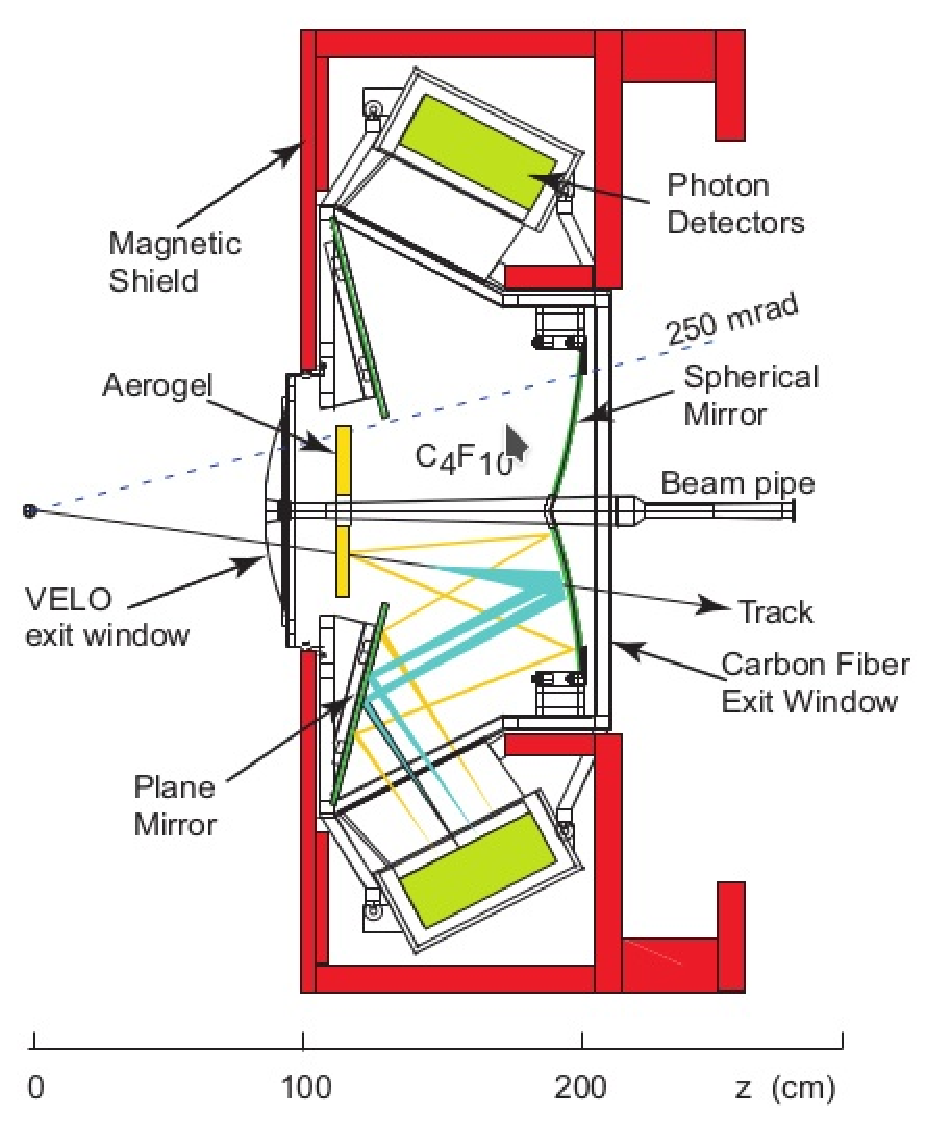
\includegraphics[width = 0.4\textwidth]{figs/detector/mechrich.eps}%
	\includegraphics[width = 0.4\textwidth]{figs/detector/license/Rich_croped.pdf}\put(-10,170){(b)}%
	\caption{ (a) Separation power for different species of particles in \DIFaddbeginFL \DIFaddFL{the }\DIFaddendFL momentum-\v{C}erenkov angle plane for \DIFaddbeginFL \DIFaddFL{the }\DIFaddendFL $\rm{C_{4}F_{10}}$ radiator. Figure from \cite{LHCb-DP-2012-003}. (b) Schematic diagram of \gls{RICH1} layout. Figure from \cite{det_paper}.}
	\label{fig:richres}
\end{figure}

\section{RICH Reconstruction and Performance }
In order to \DIFdelbegin \DIFdel{establish }\DIFdelend \DIFaddbegin \DIFadd{correctly associate }\DIFaddend species of particles \DIFdelbegin \DIFdel{for each }\DIFdelend \DIFaddbegin \DIFadd{to a given }\DIFaddend track, the \v{C}erenkov angle is combined with the track momentum measured by tracking. In practice, however, as \Gls{RICH} detectors operate in high track density environment, many \v{C}erenkov rings will be overlapping and hence a complex pattern recognition algorithm is deployed \cite{Forty:1999sg}. 


For each event, the \Gls{RICH} computes a full event likelihood that is consistent with assigning a pion mass hypothesis to all tracks given the observed hit distribution read out by the \Gls{HPD}s. The algorithm then iterates through all other possible particle species, ($e, \mu, \pi, K,$ proton, deuteron), assigning a new full event likelihood for a given track, \DIFdelbegin \DIFdel{having }\DIFdelend \DIFaddbegin \DIFadd{with }\DIFaddend all other hypotheses fixed. The mass hypothesis with the highest full event likelihood is assigned to the track and this process is repeated for all the tracks in the event, until no improvement is found. 

Results of this algorithm provide likelihood variables, $\rm{\textrm{DLL{x}}}$, that quantify the strength of the chosen species hypothesis against the pion hypothesis,
\begin{equation}
	\textrm{\textrm{DLL{x}}} = \mathrm{log}(\mathcal{L})_{x} - \mathrm{log}(\mathcal{L})_{\pi} \quad  x\in{e, \mu, K, \rm{proton, deuteron}}.
\end{equation}

By calculating $\rm{DLL{x_{1}} - DLL{x_{2}}}$, one can obtain discriminative strength between any two species.

\subsection{RICH Performance}
\label{RICHperf}
In order to measure the performance of the \Gls{PID} computed by a \gls{RICH}, populous calibration samples with very little background contamination are required. In order not to bias results, these samples have no \Gls{PID} constraints themselves and are reconstructed solely using kinematic information. For studies of pion/kaon efficiencies, $D^{*+} \to D^{0}(\kaon^{-}\pip)\pip$ backround-substracted samples are used, whereby the daughter tracks of \DIFaddbegin \DIFadd{the }\DIFaddend $D^{0}$ become proxies for the evaluation. The invariant mass for the $D^{0}$ candidates can be seen in~\autoref{fig:richperf}(a)\DIFaddbegin \DIFadd{. }\DIFaddend The probability of correctly identifying a kaon given a certain constraint on $\textrm{DLL{K}}$, \DIFaddbegin \DIFadd{the }\DIFaddend identification efficiency (\Gls{ID}), and \DIFaddbegin \DIFadd{the }\DIFaddend probability of mistakenly swapping pion identification, \DIFaddbegin \DIFadd{the }\DIFaddend misidentification efficiency (\gls{misID}), are summarized in~\autoref{fig:richperf}(b). Identification probabilities of $\approx$ 85\% with \DIFaddbegin \DIFadd{a }\DIFaddend misID rate of $\approx$ 3\% provide invaluable discriminating separation between kaons and pions.




\begin{figure}[!h]
	\centering
	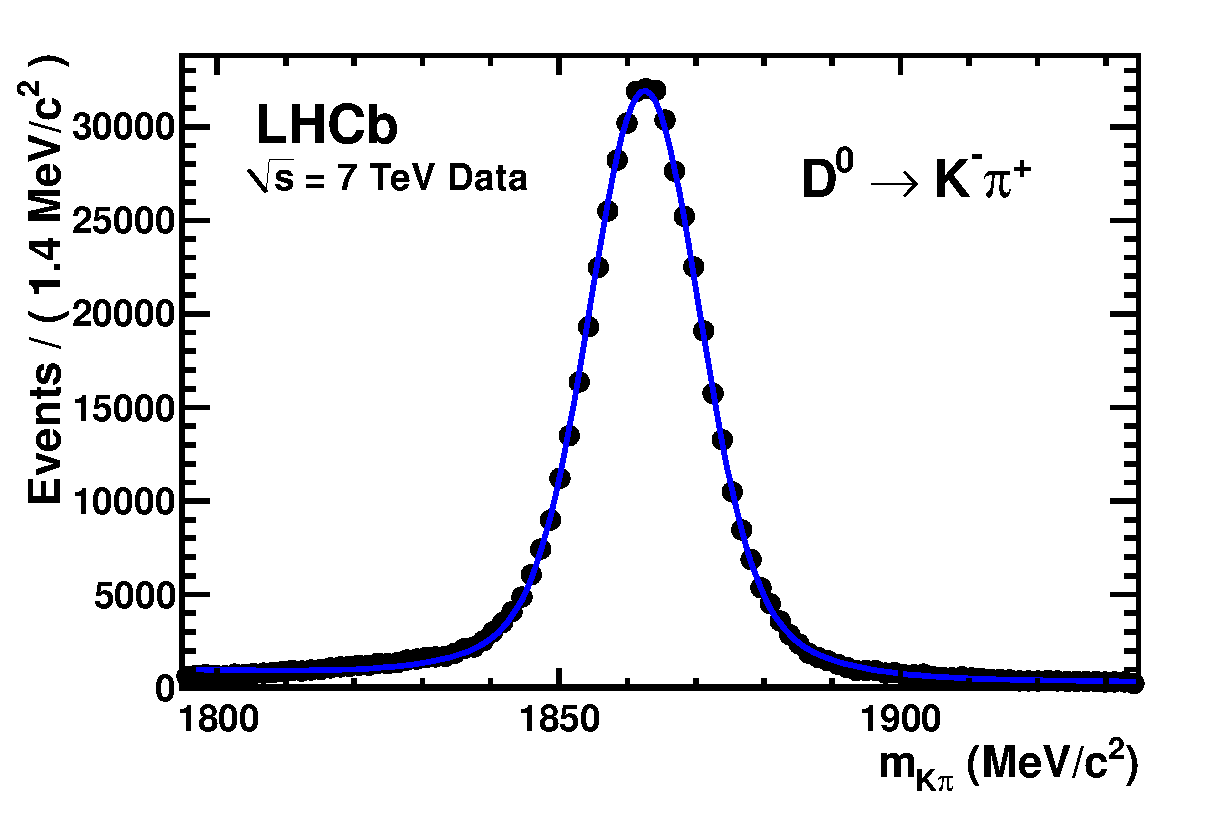
\includegraphics[width = 0.525\textwidth]{figs/detector/D0_Mass.eps}\put(-50,80){(a)}%
	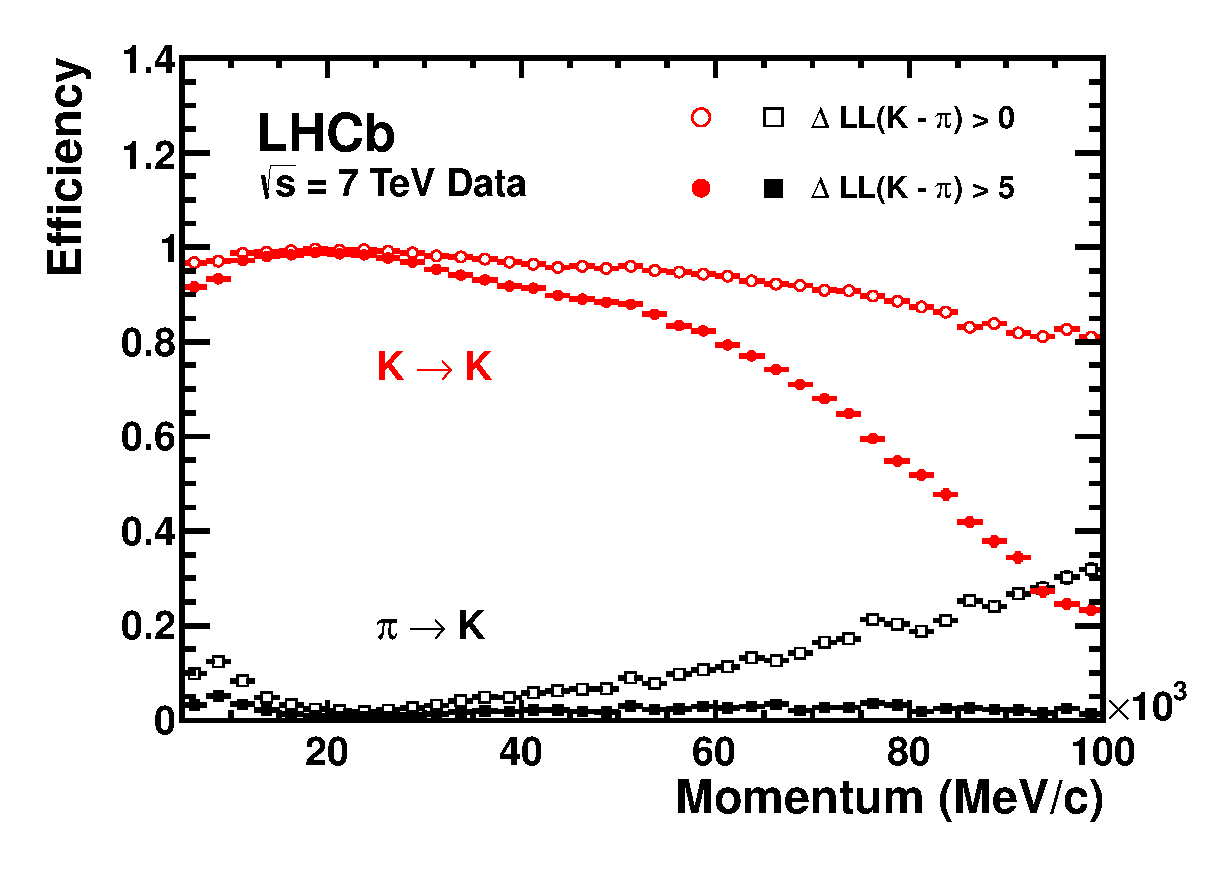
\includegraphics[width = 0.5\textwidth]{figs/detector/KandPi_2_K.eps}\put(-50,80){(b)}%
	\caption{ (a) Invariant mass distribution of $D^{0}$ data sample (in black) overlaid with fit to both background and signal (in blue). (b) An example of kaon ID (red) and misID (black) efficiency as a function of momentum under two \gls{PID} hypotheses, $\textrm{DLL{K}} > 0$ (empty)  and $\textrm{DLL{K}} > 5$ (filled). Both Figures from \cite{LHCb-DP-2012-003}.}
	\label{fig:richperf}
\end{figure}

%In search for $B^{0}$ and $B^{0}_{s}$ decaying to $h^{+}h^{-}$, where $h\in K, \pi$, $\pi^{+} \pi^{-}$ invariant mass spectra with and without \gls{PID} $\textrm{DLL{x}}$ requirements can be seen in~\autoref{fig:richnice}. These plots clearly demonstrate increase in sensitivity searching for $B^{0} \rightarrow \pi^{+} \pi^{-}$ signal amongst other components. 

%\begin{figure}[!h]
%	\centering
%	\includegraphics[width = 0.5\textwidth]{figs/detector/b2hhnopid.png}%
%	\includegraphics[width = 0.5\textwidth]{figs/detector/b2hhpid.png}%
%	\caption{ $\pi^{+} \pi^{-}$ invariant mass distributions obtained using kinematic constraints only (left) and also using \gls{PID} constraints (right) in order to isolate $B^{0} \rightarrow \pi^{+} \pi^{-}$ peak. This figure is taken from \cite{LHCb-PAPER-2012-002}. }  
%	\label{fig:richnice}
%\end{figure}


\section{Calorimetry }
\label{calosys}
As many other particle physics detectors, \Gls{LHCb} is equipped with series of subdetectors providing separation between electrons, pions and photons. This separation is achieved because different particles interact differently with the material, producing differently shaped showers. This part of the detector is not only integral to the way the \Gls{LHCb} trigger system works but it also provides a measurement of \DIFaddbegin \DIFadd{the }\DIFaddend energies of these objects.
All the subcomponents discussed here operate on the same principle. \DIFdelbegin \DIFdel{Passing particles }\DIFdelend \DIFaddbegin \DIFadd{Particles passing }\DIFaddend through the material emit light. The light from the scintillating material, which is created by absorbing the energy of the \DIFdelbegin \DIFdel{passing }\DIFdelend particle and re-emitted it in \DIFaddbegin \DIFadd{the }\DIFaddend form of light, is guided to photomultiplier tubes by wavelength shifting fibres.

Electrons, pions and photons firstly encounter two planes of scintillating tiles: the Scintillating Pad Detector (\Gls{SPD}), and the Preshower Detector (\Gls{PRS}) intersected by a wall of lead. The \Gls{SPD} senses the passage of charged particles as they emit light whereas neutral particles do not, making this subdetector \DIFaddbegin \DIFadd{able to }\DIFaddend distinguish between electrons and photons. The wall of lead initiates the electromagnetic shower, where photons are converted into electron-positron pairs, depositing sizable energy in the \Gls{PRS} allowing electron/pion separation. 

The Electromagnetic Calorimeter (\Gls{ECAL}) in \gls{LHCb} is based on a sampling shashlik-type technology, where scintillating tiles are alternated \DIFdelbegin \DIFdel{by }\DIFdelend \DIFaddbegin \DIFadd{with }\DIFaddend lead plates measuring the energy deposit of electromagnetic showers. As the best energy resolution requires full energy deposit of energetic photons along the \Gls{ECAL}, the thickness is equivalent to 25 radiation lengths. The resulting resolution of the \Gls{ECAL} is $\frac{\sigma_{E}}{E} = \frac{10\%}{\sqrt{E}} \oplus 1\%$, where $E$ is in \gev.

On the other hand, the Hadronic Calorimeter \Gls{HCAL} sandwiches iron instead of lead as the absorber with \DIFaddbegin \DIFadd{a }\DIFaddend thickness of 5.6 interaction length only, achieving a resolution of $\frac{\sigma_{E}}{E} = \frac{70\%}{\sqrt{E}} \oplus 10\%$ in beam tests. This poorer resolution however fulfils the requirements necessary for the main purpose of this detector, which is the hadron trigger. Away from the beampipe the granularity of cells is coarser to mirror the track occupancy as seen in~\autoref{fig:CaloGran}(a)(b). 

\begin{figure}[!h]
	\centering
	\includegraphics[width = 0.5\textwidth]{figs/detector/license/ECAL_crop.pdf}\put(-70,10){(a)}%%
	\includegraphics[width = 0.5\textwidth]{figs/detector/license/HCAL_crop.pdf}\put(-70,10){(b)}%%
	\caption{Granularity of (a) \Gls{ECAL} and (b) \Gls{HCAL} detectors. This is just a quarter view and that the black region is where the beam pipe is located. Figure from \cite{det_paper}. }  
	\label{fig:CaloGran}
\end{figure}




\section{Muon Stations }
\label{muonsys}
Muons are considered to be of fundamental importance to many flagship analyses by \Gls{LHCb}, such as the search for the rare $\B^{0}_{s} \rightarrow \mu^{+} \mu^{-}$ decay\cite{Aaij:2017vad}. Analysis of \Bmumumu of course relies heavily on \DIFaddbegin \DIFadd{a }\DIFaddend good performance of this part of \DIFaddbegin \DIFadd{the }\DIFaddend detector. Muon stations are positioned at the end of the detector, taking advantage of the fact that muons penetrate material better than any other particle type. 

\Gls{LHCb}'s five rectangular muon stations \Gls{muonstation} are positioned before and after \DIFaddbegin \DIFadd{the }\DIFaddend calorimetry system, with \DIFaddbegin \DIFadd{the }\DIFaddend first station M1 upstream of the \Gls{SPD}, and four stations (M2-M5) downstream of \Gls{HCAL} as shown in~\autoref{fig:MuonGran}. The M1 station consists of 12 sets of three gas electron 
multiplier foils (triple-GEMs) in the region closest to the beam pipe, resisting the highest dose of radiation due to the highest particle flux. Its main use lies in improving the measurement of $p_{T}$ in the hardware trigger. The M2-M5 stations each consist of 276 multi-wire proportional chambers (\Gls{MWPCs}) filled with an $\rm{Ar,CO_{2},CF_{4}}$ gas mixture. They are interlayered with 0.8\m iron walls, to provide a stopping target for all particles, other than muons with momentum higher than $6$ \gevc.

%In order to ease the accessibility, like in \Gls{VELO}, all the stations are split into two independent mechanical sides, also known A and C side.

Each half of a muon station is segmented into four increasingly larger regions away from the beam, R1 to R4.
 All the regions were constructed to cover the same acceptance, keeping the track occupancy constant across the station. The granularity of the readout is higher in the horizontal plane to take advantage of the magnet's horizontal bending plane.




\begin{figure}[!h]
	\centering
	\includegraphics[width = 1.0\textwidth]{figs/detector/sideview.pdf}%
	%\includegraphics[width = 0.5\textwidth]{figs/detector/b2hhpid.png}%
	\caption{(a) Layout of the muon detector x-z plane and (b) x-y plane. Figure from \cite{LHCb-DP-2012-002}. }  
	\label{fig:MuonGran}
\end{figure}

Both GEM and \Gls{MWPCs} operate on \DIFdelbegin \DIFdel{a }\DIFdelend \DIFaddbegin \DIFadd{the }\DIFaddend same principle. In each station, the position in the $x-y$ plane is determined by ionizing electrons that come from muons passing through the detector, which are then attracted either to the closest anode mesh or wire mesh. The trigger is fired if the corresponding rectangular region in each station registered a positive binary decision. This means \DIFdelbegin \DIFdel{an }\DIFdelend \DIFaddbegin \DIFadd{the }\DIFaddend efficiency of each station must be $\geq$99\% to give \DIFaddbegin \DIFadd{an }\DIFaddend overall 95\% trigger efficiency. %Geometrical layout covers $\approx$ 20\% muons originating in semileptonic $b$ decays.\mybox{\color{red}CERN-THESIS-2012-025.pdf from puig, i have to invedtigate}


\subsection{Muon Identification }
\label{muonID}
Apart from triggering events with high enough $p_{T}$ muons, the muon stations provide necessary \gls{PID} information for muon analyses. Offline variables mostly used for muon ID by analysts are
 \begin{itemize} 
	\DIFdelbegin %DIFDELCMD < \item{\textbf{IsMuon}: Boolean decision of muon candidates with momentum-dependent categorisation. Long tracks with $p>3$\gev/c are extrapolated to muon stations yielding $x-y$ coordinates in M2-M5, considering only tracks within acceptance. For each station, a search for hit information within an elliptical area defined by momentum, a field of interest (\Gls{FOI}), is performed. The hit requirements are summarized in~\autoref{tab:ismuontab}.}
%DIFDELCMD < 	\item{\textbf{muDLL}: Difference in log likelihoods computed using muon and non-muon hypothesis. These hypotheses are based on the proximity/distance $D^{2}$ of the track extrapolation into the muon stations and corresponding closest sensed hits in those stations. Muon-like particle will tend to have sharper distribution in $D^{2}$ as compared to other species. Protons were chosen to be the other species for the calibration purposes. They give a broader distribution as they originate either as punch-through protons (protons coming from showers not fully contained in the \gls{HCAL}), protons having coincident hit position to a true muon, or random hits.}
%DIFDELCMD < 	%%%
\DIFdelend \DIFaddbegin \item{\textbf{IsMuon}: Boolean decision of muon candidates with momentum-dependent categorisation. Long tracks with $p>3$\gev/c are extrapolated to muon stations yielding $x-y$ coordinates in M2-M5, considering only tracks within the acceptance. For each station, a search for hit information within an elliptical area defined by momentum, a field of interest (\Gls{FOI}), is performed. The hit requirements are summarized in~\autoref{tab:ismuontab}.}
	\item{\textbf{muDLL}: Difference in log likelihoods computed using a muon and non-muon hypothesis. These hypotheses are based on the prox imity/distance, $D^{2}$, of the track extrapolation into the muon stations and corresponding closest sensed hits in those stations. Muon-like particles will tend to have a sharper distribution in $D^{2}$ as compared to other species. Protons were chosen to be the other species for the calibration purposes. They give a broader distribution as they originate either as punch-through protons (protons coming from showers not fully contained in the \gls{HCAL}), protons having the same hit position as true muon, or random hits.}
	\DIFaddend \item{\textbf{DLLmu}}:  For each track \DIFdelbegin \DIFdel{a }\DIFdelend \DIFaddbegin \DIFadd{the same }\DIFaddend global likelihood is produced, by \DIFdelbegin \DIFdel{combination of }\DIFdelend \DIFaddbegin \DIFadd{combining the }\DIFaddend muon and non-muon \DIFdelbegin \DIFdel{likelihood }\DIFdelend \DIFaddbegin \DIFadd{likelihoods }\DIFaddend from \textbf{muDLL}, with the \Gls{RICH} different mass hypothesis likelihoods, and \DIFaddbegin \DIFadd{the }\DIFaddend calorimetry likelihood exploiting \DIFaddbegin \DIFadd{information about }\DIFaddend the energy deposits\DIFdelbegin \DIFdel{information}\DIFdelend . Like in the \Gls{RICH} likelihoods, the default hypothesis corresponds to separation between the muon and pion hypotheses.    

 \end{itemize} 

\noindent \DIFdelbegin \DIFdel{Other variables which are extensively }\DIFdelend \DIFaddbegin \DIFadd{In the }\Bmumumu \DIFadd{analysis }\texttt{\DIFadd{IsMuon}} \DIFadd{and }\texttt{\DIFadd{DLLmu}} \DIFadd{variables are used to identify muons. On the top, other variables, which are }\DIFaddend used for muon \DIFdelbegin \DIFdel{particle identification in }\DIFdelend \DIFaddbegin \DIFadd{identification in the }\DIFaddend search for \Bmumumu\DIFaddbegin \DIFadd{, }\DIFaddend are described in~\autoref{otherpid}. \DIFaddbegin \DIFadd{The use of several variables for muon identification is done as they are mostly complimentary, exploiting different information from different parts of the detector. 
}\DIFaddend 

\begin{table}[!h]
	\centering
	\hspace*{-0.8cm}
	\begin{tabular}{c c}
		\toprule
		Particle Momentum $p$  & Hits in Muon Stations \\ \hline
		3 \gev/c <$p$<6 \gev/c & M1 $\&$ M2\\
		6 \gev/c <$p$<10 \gev/c & M1 $\&$ M2 $\&$ (M3 $||$ M4) \\
		10 \gev/c <$p$ & M1, M2, M3 and M4 \\ \bottomrule      
	\end{tabular}
	\caption{Momentum-dependent definition \texttt{IsMuon} variable.}
	\label{tab:ismuontab}
\end{table}   

\subsection{Muon Identification Performance}
\label{muonperf}
As for hadron performance measurements, the muon ID performance is determined using the high statistics decay channel $J/\psi \rightarrow \mu^{+} \mu^{-}$ with a \textit{tag and probe} method. MisID rates \DIFdelbegin \DIFdel{of }\DIFdelend \DIFaddbegin \DIFadd{for }\DIFaddend kaons and pions are computed using the same decay channels, which were used for \DIFaddbegin \DIFadd{the }\DIFaddend identification of hadrons, $D^{*+} \to D^{0}(\kaon^{-}\pip)\pip$. The summary of \texttt{IsMuon} ID and misID rates are presented in~\autoref{fig:MuonID}. \DIFdelbegin \DIFdel{Very }\DIFdelend \DIFaddbegin \DIFadd{A very }\DIFaddend high ID rate (above 90\%) for relatively low misID probability (below 10\%) is key to analyses with muons in \DIFdelbegin \DIFdel{a }\DIFdelend \DIFaddbegin \DIFadd{the }\DIFaddend final state. \DIFdelbegin \DIFdel{But the least performing are the }\DIFdelend \DIFaddbegin \DIFadd{The identification rate for the }\DIFaddend low $p_{T}$ muons \DIFdelbegin \DIFdel{where the identification }\DIFdelend suffers because these muons can end up outside of the \gls{LHCb} acceptance\DIFdelbegin \DIFdel{and misID }\DIFdelend \DIFaddbegin \DIFadd{. MisID }\DIFaddend rates for kaon and pions are significantly higher in \DIFaddbegin \DIFadd{the }\DIFaddend low momenta region as the dominant process \DIFdelbegin \DIFdel{causing this are }\DIFdelend \DIFaddbegin \DIFadd{for this occurence is }\DIFaddend muons from decay-in-flight.   

\begin{figure}[!h]
	\includegraphics[width = 0.5\textwidth]{figs/detector/dllFit_mu_IMvsPvsPt.pdf}%
	\includegraphics[width = 0.5\textwidth]{figs/detector/dllFit_P_IMvsPvsPt.pdf}%
       \newline
	\includegraphics[width = 0.5\textwidth]{figs/detector/dllFit_pi_IMvsPvsPt.pdf}%
	\includegraphics[width = 0.5\textwidth]{figs/detector/dllFit_ka_IMvsPvsPt.pdf}%
	\caption{(a) Probability of correctly identifying muons as a function of momentum \DIFdelbeginFL \DIFdelFL{$p$ }\DIFdelendFL in \DIFdelbeginFL \DIFdelFL{the }\DIFdelendFL bins of $p_{T}$ for $J/\psi \rightarrow \mu^{+} \mu^{-}$ with \DIFaddbeginFL \DIFaddFL{an }\DIFaddendFL \texttt{IsMuon} constraint. (c) Probability of incorrectly identifying \DIFaddbeginFL \DIFaddFL{a }\DIFaddendFL pion (b) proton and (d) kaon as \DIFaddbeginFL \DIFaddFL{a }\DIFaddendFL muon with \texttt{IsMuon}. This figure is taken from \cite{LHCb-DP-2013-001}. }  
	\label{fig:MuonID}
\end{figure}


\section{Trigger }
\label{triggerchap}
Big-data physics experiments have to make decisions on what kind of data they want to keep. The choice of interesting events is performed by a series of decisions, which is known as the trigger. The \Gls{LHCb} trigger system was build around constraints posed by the run conditions, read-out capabilities and available disk space. In Run \Rn{1} and Run \Rn{2} \gls{LHCb} has at its disposal the multistage trigger consisting of a hardware-based level 0 trigger (\Gls{L0}) and a software-based high level trigger (\Gls{HLT}).

In the end, selected events have their trigger decisions categorized. An event where the signal candidate caused the trigger to fire is known \DIFdelbegin \DIFdel{to be }\DIFdelend \DIFaddbegin \DIFadd{as }\DIFaddend Trigger on Signal (\Gls{TOS}). An event where it is a non-signal like particle causing the trigger decision to occur \DIFdelbegin \DIFdel{, }\DIFdelend \DIFaddbegin \DIFadd{is labelled as }\DIFaddend Trigger Independent of Signal (\Gls{TIS})\DIFdelbegin \DIFdel{is labelled}\DIFdelend . Finally, if only \DIFdelbegin \DIFdel{by }\DIFdelend a combination of signal particle(s) together with other \DIFdelbegin \DIFdel{particle's properties }\DIFdelend \DIFaddbegin \DIFadd{particles }\DIFaddend in the event \DIFdelbegin \DIFdel{produce }\DIFdelend \DIFaddbegin \DIFadd{produces }\DIFaddend an affirmative decision, then these events are categorized as \Gls{TIS} $\&$ \Gls{TOS} = \Gls{TISTOS}.

\Gls{L0} reduces the rate of data from 40 \mhz to 1 \mhz by employing five trigger decisions, also known as lines. The first three lines make \DIFaddbegin \DIFadd{a }\DIFaddend decision using calorimeter information about the transverse energy, $E_{T}$, \DIFaddbegin \DIFadd{and }\DIFaddend whether it is \DIFaddbegin \DIFadd{a }\DIFaddend photon, electron or hadron causing the shower energy deposit. Two other lines \DIFdelbegin \DIFdel{are reading }\DIFdelend \DIFaddbegin \DIFadd{read }\DIFaddend out information from the muon system by looking for  \DIFdelbegin \DIFdel{transverse momentum, }\DIFdelend $p_{T}$, of muon and dimuon (two muon tracks) objects. \DIFdelbegin \DIFdel{Efficiencies }\DIFdelend \DIFaddbegin \DIFadd{The efficiencies }\DIFaddend of the L0 muon triggers are evaluated using $B^{+} \rightarrow (J/\psi \rightarrow \mu^{+} \mu^{-}) K^{+}$ decays and can be seen in~\autoref{fig:L0Perf}(a). The hadron trigger efficiency in different decay channels can be seen in~\autoref{fig:L0Perf}(b). 


\begin{figure}[!h]
	\centering
	\includegraphics[width = 0.5\textwidth]{figs/detector/Fig1_L0MuonEff_PT.pdf}\put(-50,90){(a)}%
	\includegraphics[width = 0.5\textwidth]{figs/detector/Fig21_L0Hadron_PT.pdf}\put(-50,90){(b)}%
	%\includegraphics[width = 0.5\textwidth]{figs/detector/b2hhpid.png}%
	\caption{ (a) \Gls{TOS} efficiency as a function of $p_{T}$ for muon-based decisions. (b) \Gls{TOS} efficiency for different decays using L0 hadron trigger lines. Figures from \cite{Albrecht:2013fba}. }  
	\label{fig:L0Perf}
\end{figure}


 The software-based \Gls{HLT} then further reduces the rate from 1 \mhz down to $5$ \khz which can be recorded to long-term storage. The first stage of the \Gls{HLT}, (\Gls{HLT1}), performs limited track reconstruction and hence makes a decision based on the presence of charged particles in the event. \Gls{HLT1} uses \Gls{VELO} hits to reconstruct \Gls{PV}s and \Gls{VELO} tracks by using 3D pattern recognition. As \Gls{LHCb}'s primary mission is to study decays of hadrons containing $b$ and $c$ quark, \Gls{HLT1} will make \DIFaddbegin \DIFadd{a }\DIFaddend decision based on the track being displaced (having \DIFaddbegin \DIFadd{a }\DIFaddend high \Gls{IP}) with respect to the \Gls{PV}. For events selected by the \texttt{L0Muon}, an attempt is made to match the \Gls{VELO} tracks to hits observed in the vertical plane in the muon chambers, where the magnetic field of the dipole will not make them bend. By computing the track $\chi^2$, the potential muon track candidates are selected. Finally, the \Gls{VELO} tracks and muon tracks are extrapolated into the \Gls{OT} or \Gls{IT} trackers, allowing for so called \textit{forward tracking}, whereby $p$ and $p_{T}$ requirements are imposed to reduce processing time. Each track is then fitted with  a fast Kalman filter providing the $\chi^2$ of the fit. The corresponding performance of \DIFaddbegin \DIFadd{the }\DIFaddend \Gls{HLT1} trigger lines are shown in~\autoref{fig:Hlt1Perf}(a)(b).


\begin{figure}[!h]
	\centering
	\includegraphics[width = 0.5\textwidth]{figs/detector/Fig3_Hlt1MuonEff_PT.pdf}\put(-50,140){(a)}%
	\includegraphics[width = 0.5\textwidth]{figs/detector/Fig5_Hlt1TrackAllL0_PT.pdf}\put(-50,140){(b)}%
	%\includegraphics[width = 0.5\textwidth]{figs/detector/b2hhpid.png}%
	\caption{ \Gls{HLT1} efficiencies of the corresponding triggers using the same proxy as in~\autoref{fig:L0Perf}. Figures from \cite{Albrecht:2013fba}. }  
	\label{fig:Hlt1Perf}
\end{figure}

The second stage \Gls{HLT2} reduces the rate to 5 \khz that can be safely written to disk. \Gls{HLT2} consists of a series of decisions based on a full reconstruction of either groups of decays or specific decay modes. \textit{Topological triggers} exploit the vertex and track information (topology) of $b$-hadron decays. By employing multivariate techniques 2-,3- or 4-body decays that are well separated from the \Gls{PV} are reconstructed. To account for decays where a final state particle is not fully reconstructed, the corrected mass (will be defined in~\autoref{eq:corrm}) serves as an input variable in the the \Gls{BDT}. Dedicated lines are also written to reconstruct muon and dimuon channels allowing for both prompt $J/\psi$ and $B\rightarrow J/\psi X$ studies. Finally there are \textit{Exclusive triggers} concentrating on selecting events with $D$ mesons. They perform \DIFaddbegin \DIFadd{a }\DIFaddend selection which is very similar to the offline selection but without \Gls{PID} cuts.% and with \textit{prescales} required, where only a certain fraction of events is allowed to pass through.



Between the Run \Rn{1} and Run \Rn{2} period there has been a change in how the software trigger operates, which can be seen in~\autoref{fig:TriggerChange}. As more computing resources were introduced for both \Gls{HLT1} and \Gls{HLT2}, \Gls{LHCb} took advantage in upgrading the trigger system by introducing an update of \DIFaddbegin \DIFadd{the }\DIFaddend calibration and alignment constants of the relevant subdetectors before the data is sent to permanent disk. \textit{Online reconstruction}, defined as being produced at the trigger farm, became the same as the \textit{offline reconstruction}, defined as reconstruction made when data reached the permanent disk. Hence, there is \DIFdelbegin \DIFdel{enhancement of }\DIFdelend \DIFaddbegin \DIFadd{an enhancement of the }\DIFaddend available information, such as the \Gls{PID} in the \Gls{HLT}, which can then be used at the trigger level. 


\begin{figure}[!h]
	\centering
	\includegraphics[width = 0.5\textwidth]{figs/detector/LHCb_Trigger_RunIAlg.pdf}%
	\includegraphics[width = 0.5\textwidth]{figs/detector/LHCb_Trigger_RunII.pdf}%
	%\includegraphics[width = 0.5\textwidth]{figs/detector/b2hhpid.png}%
	\caption{Trigger scheme differences between Run \Rn{1} and Run \Rn{2}. Figures from \cite{triggerscheme}.}  
	\label{fig:TriggerChange}
\end{figure}


\section{Simulation }
\label{simulationchap}
In order to optimise the event selections, determine efficiencies and model the backgrounds, a full Monte Carlo Simulation \Gls{MC} can be produced starting from simulation of the $pp$ collision to detector readout of the decay of interest produced. 
The $pp$ collisions within the \Gls{LHCb} configuration \cite{Belyaev:2011zza} are simulated with Pythia 6.4 \cite{pythia6} and Pythia 8.1 \cite{pythia8}. \Gls{LHCb} specific settings are mostly related to running conditions: luminosity, number of collisions per bunch crossing as well as contamination from other bunches, \textit{spill-over}. 

In the $pp$ collision, the $b$ and $c$ production mechanisms are simulated and then the following $b\bar{b}$ or $c\bar{c}$ pair is hadronized into hadrons of interest. In this thesis and the analysis presented, the \Bp meson is the hadron of interest. Hadrons are then further decayed using EVTGEN \cite{Lange:2001uf} into the chosen decay products. At this stage, different physics models or inputs from theory can be configured. % At the same time some initial CPU-friendly selection is established, usually requiring the hadrons to be contained within the forward detector's acceptance.
In order to account for the effects of \Gls{QED} radiative corrections, the PHOTOS \cite{photos} algorithm can be used. All of this combined establishes \textit{the generator-level simulation} of LHCb.


In the next phase, \textit{detector simulation}, the interactions of \DIFdelbegin \DIFdel{the }\DIFdelend all the particles with the detector, transport, as well as detector's response are simulated using the C++ GEANT4 toolkit \cite{Geant4},\cite{Agostinelli:2002hh}. \Gls{LHCb}'s interface to GEANT4 is detailed in Ref\cite{Clemencic:2011zza}. 

\subsection{Differences in Simulation and Data}
\label{detpid}
Despite the complexity and best intention of the \Gls{LHCb} simulation, there are several shortcomings that require corrections.
The most affected variables necessary for physics analyses that one needs to consider are \Gls{IP} resolution, track reconstruction efficiencies, \Gls{PID} variables and track occupancy.

The \Gls{IP} resolution shows a better trend in the simulation then in the data due to the mismodelling of the material description \DIFdelbegin \DIFdel{of }\DIFdelend \DIFaddbegin \DIFadd{in }\DIFaddend the \Gls{VELO} simulation. As shown in~\autoref{fig:IPRES}(a)(b)  the \Gls{IP} resolution does greatly differ depending \DIFaddbegin \DIFadd{on }\DIFaddend the variation of material density of \Gls{VELO}. Around $\phi=\pm\pi/2$, where the two \Gls{VELO} parts overlap, the material difference causes the discrepancy. It can be corrected either by reweighting to data or by smearing the resolution with a Gaussian distribution.

\begin{figure}[!h]
	\centering
	\includegraphics[width = 0.5\textwidth]{figs/detector/IPXRes-Vs-InversePT-Compare2012DataToMC.pdf}\put(-50,60){(a)}%
	\includegraphics[width = 0.5\textwidth]{figs/detector/IPXRes-Vs-Phi-Compare2011DataToMC.pdf}\put(-50,60){(b)}%
	\caption{ (a) \Gls{IP} resolution in \DIFaddbeginFL \DIFaddFL{the }\DIFaddendFL x-direction comparing the data and simulation \DIFdelbeginFL \DIFdelFL{output }\DIFdelendFL for \DIFaddbeginFL \DIFaddFL{the }\DIFaddendFL 2012 data-taking period. (b) \Gls{IP} resolution in \DIFaddbeginFL \DIFaddFL{the }\DIFaddendFL x-direction comparing the data and simulation \DIFdelbeginFL \DIFdelFL{output }\DIFdelendFL for \DIFaddbeginFL \DIFaddFL{the }\DIFaddendFL 2011 data-taking period as a function of angle, $\phi$. Figures from \cite{LHCbVELOGroup:2014uea}. }  
	\label{fig:IPRES}
\end{figure}


Track reconstruction efficiency is also not reproduced very well in certain \DIFdelbegin \DIFdel{kinematical }\DIFdelend \DIFaddbegin \DIFadd{kinematic }\DIFaddend bins, again due to modelling of scattering interactions.

The most critical problem that needs to be addressed in the presented analysis \DIFdelbegin \DIFdel{are }\DIFdelend \DIFaddbegin \DIFadd{is }\DIFaddend the inaccuracies of the \Gls{PID} variables, which are mismodelled in the simulation. \DIFdelbegin \DIFdel{The origin of this }\DIFdelend \DIFaddbegin \DIFadd{This }\DIFaddend problem arises as a consequence of \DIFaddbegin \DIFadd{the }\DIFaddend much lower estimate of low momentum tracks in the detector\DIFaddbegin \DIFadd{, }\DIFaddend making the photoelectron background underestimated. This results in better \DIFdelbegin \DIFdel{performance of separation power }\DIFdelend \DIFaddbegin \DIFadd{separation }\DIFaddend in simulation and is corrected using \DIFaddbegin \DIFadd{a }\DIFaddend data calibration. 

Therefore the \gls{PID} efficiency is usually obtained from \DIFaddbegin \DIFadd{the }\DIFaddend data. More specifically, this is done by using high-yield and relatively background-free calibration channels, where the species of the particle can be deduced from kinematics of the decay. \DIFdelbegin \DIFdel{Standard }\DIFdelend \DIFaddbegin \DIFadd{A standard }\DIFaddend set of these channels are "housed" in a \texttt{PIDCalib} package \cite{Anderlini:2202412}. \DIFdelbegin \DIFdel{In }\DIFdelend \DIFaddbegin \DIFadd{With }\DIFaddend this package, \DIFaddbegin \DIFadd{the }\DIFaddend \gls{PID} efficiency can be computed in a given kinematic region of interest. 



%%%\thesubsection{Boosted Decision Trees}
\label{app:bdt}
%% As the HLT trigger makes use of a machine learning technique called a Boosted Decision Trees (BDT), an aside will be taken here to introduce the concept.

Many rare decay analyses make extensive use of BDTs and they are important in the \Lbpi analysis. Firstly, the concept of a decision tree is introduced followed by a brief explanation of boosted decision trees.

A decision tree, in the context of data mining, is a supervised machine learning method which allows for the prediction of the value of a target variable based on several input variables. In particle physics, the purpose of the decision tree is to classify an event as being either signal or background, based on the event's input variables. The input variables, $\left\{x_{i}\right\}$, are various physics parameters. % and in the case of the HLT include the minimum $P_{T}$  and mass of the particle.
% and $IP_{\chi2}$ (where the $IP_{\chi2}$ is the difference in the $\chi2$ of the fit to the PV when the track whose $IP_{\chi2}$ is being measured is added and then removed)
Each cut point in the tree is referred to as a node and the final nodes are referred to as leaves. A very simple example is shown in~\autoref{fig:BDT}. The purity, $P$, of a leaf refers to the fraction of the weight of a leaf due to signal events, e.g. if a leaf had 20 signal events and 15 background events it would have a purity of 0.75. If a leaf has a purity larger than 0.5 it is deemed to correspond to signal and if lower, to background.
\begin{figure}
  \centering
  \includegraphics[scale = 0.7]{figs/BDT.png}
  \caption{An example decision tree. The S and B stand for `Signal-like' and `Background-like'. The $\beta_{i}$ variables refer to the cut values chosen by the machine learning algorithm after the tree has been trained on signal and background samples. The blue ovals represent final nodes called leafs, which each leaf having an associated purity, i.e. the fraction of the weight of a leaf due to signal events.}
  \label{fig:BDT}
\end{figure}

A decision tree is constructed by a process called training. For this, samples of known signal and background events are used. These samples could be either simulation or data. For each $x_{i}$ the best dividing point is decided, that is, the cut that gives the best separation between signal and background. This optimum point is decided by using the Gini index defined as

\begin{equation}
Gini  = \sum^{n}_{i = 1} W_{i} P(1 - P),
\end{equation}
where $W_{i}$ is weight of the $i^{th}$ event, which would generally be unity for the case of a non-boosted decision tree. 
The cutting point is then found by maximising the separation, $\Delta$, between the Gini index of the parent node and the combined Gini index of the child nodes, as given in~\autoref{eq:diffgini} 
\begin{equation}
 \Delta =   Gini_{parent} - Gini_{child_{1}} - Gini_{child_{2}}.
  \label{eq:diffgini}
\end{equation}
The depth of a tree (the maximum number of cuts or nodes) is normally a number specified before the training begins.
%\cite{miniboone}

Boosting a decision tree involves training many trees ($\mathcal{O} \sim 1000$) and giving misclassified events a higher weight. A misclassified event is defined as a known signal event being placed on a background leaf and vice versa. By giving the events which are difficult to classify more weight, the next tree to be trained will effectively have to work harder in order to classify events correctly. %The way in which events are weighted (or boosted) can vary, and in the 

The total score on an event is deduced by following an event through from tree to tree and, for the algorithms used in this thesis, is simply given by the weighted sum of the scores over the individual trees.

%% This weighting is done using the total number of misclassified events in a tree. The error of the $m^{th}$ tree is defined as
%% \begin{equation}
%%   err_{m}=\sum_{j}W_{j}; j = \text{misclassified event}.
%% \end{equation}
%% The weight (or score) of this tree is then given as
%% \begin{equation}
%%   \alpha_{m} = C \ln\frac{1-err_{m}}{err_{m}},
%% \end{equation}
%% where $C$ is  a constant. The increase in weight of a misclassified event is given as
%% \begin{equation}
%%   W_{i} = W_{i} e^{\alpha_{m}}.
%% \end{equation}
%% All weights are then renormalized, $W_{i} \to W_{i}/\sum^{N}_{i = 1} W_{i} $, and the total output, $T(x_{i})$, for an event $i$ is given as
%% \begin{equation}
%%   T(x_{i}) = \sum^{N_{tree}}_{m = 1} \alpha_{m}T_{m}(x_{i}).
%% \end{equation}

Data sets are split into two (or more) sub samples, where one half is used for training the tree and the other is used for testing the tree, and the distributions of the event scores (the BDT output) for training and testing samples are compared for signal and background. Cases where the training sample performs better than the testing sample are referred to as over-trained trees, which is often due to the BDT becoming sensitive to the statistical fluctuations of the training sample.%Most BDT's used within LHCb produce a BDT output ranging from -1 to 1, with more positive outputs being associated with a more signal-like data candidate.

 The distribution of events scores for a given dataset can then be cut on in order to increase the fraction of signal events.

%Alternatively, the over performance of the training sample could be due to there being correlations between the  signal and background proxies used for training which do not exist in the actual data. 
%% The value for $G$ is calcualted using the Gini index which is a function of the purity $p$.


%% The creates two new nodes and the algorithum is applied again to these nodes. Adapative boosting is when misclassfied events (i.e. in the case when you have a signal training sample the event is classified as abckground and vice versa) and given higher weighs 
%% For each xi the splitting value that gives the best separation of the events into two child nodes -- one with mostly signal events, the other with mostly background events -- is found. The variable and split value giving the best separation are selected and two new nodes are created, one corresponding to events satisfying the split criterion (labeled P for passed in the above figure), the other containing events that failed it (labeled F). The algorithm is then applied recursively to the two child nodes. This process contains untill the specified maximum number of given nodes. When the splitting stops, the terminal node is called a leaf, with an associated purity, the weighted signal fraction of the training sample in this node

%The primary vertex is defined as being within a raduis of 300\mum of the mean position of the $pp$ interation. 



\input{PIDchap_corrected}
\input{Selection2_corrected}
\chapter{Background Studies}
\label{chap:back}

%\textit{The decay \Bmumumu is a fully leptonic decay with good potential for eliminating many types of the backgrounds. In this chapter parametrisation and estimations for all considered backgrounds are sketched. A quick summary of all backgrounds that passed the stringent selection were provided in~\autoref{bkgquick}.}

\textit{In this chapter a summary of \DIFdelbegin \DIFdel{considered }\DIFdelend \DIFaddbegin \DIFadd{the }\DIFaddend backgrounds is provided with \DIFaddbegin \DIFadd{the }\DIFaddend combinatorial background described in~\autoref{combiback}, misidentified background in~\autoref{misidprocedure}, different classes of partially reconstructed background in~\autoref{partrecobak} and finally rare and resonant backgrounds in~\autoref{rareandreso}.}

\section{Combinatorial Background}
\label{combiback}
\DIFdelbegin \DIFdel{Combinatorial }\DIFdelend \DIFaddbegin \DIFadd{The combinatorial }\DIFaddend background is when a random combination of tracks from different $b$-decay chains \DIFdelbegin \DIFdel{fake }\DIFdelend \DIFaddbegin \DIFadd{fakes }\DIFaddend the signal. The usual method at \gls{LHCb} of estimating the amount and the shape of this background include extrapolation from the upper mass data sideband to the signal region. In this case, the upper mass sideband is defined as $M_{\rm{B_{corr}}} > 5500 \mevcc$ and the signal region is defined to be $ 4500 \mevcc <M_{\rm{B_{corr}}} < 5500 \mevcc$. \DIFdelbegin \DIFdel{The characteristic shape for this }\DIFdelend \DIFaddbegin \DIFadd{This }\DIFaddend background can be described by an exponential function in a certain range, where this range is the primary discussion of this section. Since the tight selection results in \DIFdelbegin \DIFdel{low-statistics }\DIFdelend \DIFaddbegin \DIFadd{small }\DIFaddend data samples, the extrapolation from the upper mass sideband introduces a large uncertainty on the exponential constant and cannot be used to estimate the correct shape and yield of this background. What can be done, however, is to assume the exponential shape for the combinatorial component and let the exponential constant be a floating parameter in the data fit. This method for estimation of the combinatorial component will be mentioned in the signal data mass fits, in~\autoref{sigpara}. 
%In the rest of this section exponential parametrisation of this background between $4000 \mevcc <M_{\rm{B_{corr}}} < 7000 \mevcc$ is motivated. This is important as the final fitting region was chosen in such a way as to make sure that combinatorial background is exponential in this entire fitting region. 

Apart from the nominal upper mass data sideband sample, two other samples are analysed as proxies for this type of background. Despite the fact that these samples are also scarcely populated, they are studied altogether to determine in which mass regions the combinatorial background can be considered exponential. Firstly, the same sign data sample was \DIFdelbegin \DIFdel{studies }\DIFdelend \DIFaddbegin \DIFadd{studied }\DIFaddend (the same sample as in~\autoref{cloniatkos})\DIFdelbegin \DIFdel{, where this }\DIFdelend \DIFaddbegin \DIFadd{. This }\DIFaddend sample consists of $\mu^{+} \mu^{+} \mu^{+} \nu$ events passing all \DIFdelbegin \DIFdel{selection up to }\DIFdelend \DIFaddbegin \DIFadd{selections up to the }\DIFaddend MVA selection to \DIFdelbegin \DIFdel{have sufficient statistics}\DIFdelend \DIFaddbegin \DIFadd{be of sufficient size}\DIFaddend . Secondly an inclusive $b\bar{b}$ simulation sample consisting of events where two muons with $p > 3$ \gevc are required to be present alongside \DIFdelbegin \DIFdel{with }\DIFdelend a third muon. On \DIFdelbegin \DIFdel{the }\DIFdelend top, these events have to satisfy all the stripping \DIFdelbegin \DIFdel{selection }\DIFdelend \DIFaddbegin \DIFadd{criteria }\DIFaddend outlined in~\autoref{tab:stripcutsB}.

As seen in~\autoref{fig:bbarcombi}(b)(c), the exponential shape is only valid for $M_{\mathrm{B_{corr}}}>4000 \mevcc$. Hence the choice of fitting region $4000 \mevcc<M_{\rm{B_{corr}}}<7000\mevcc$.

\begin{figure}[H]
\center
\includegraphics[width = 0.33\textwidth]{bkg/combi/nicenewANAcombiUMSB_WITHPULL_new.pdf}\put(-70,100){(a)}%
\includegraphics[width = 0.33\textwidth]{bkg/combi/nicenewANAcombi3same_WITHPULL_new.pdf}\put(-70,100){(b)}%
\includegraphics[width = 0.33\textwidth]{bkg/combi/nicenewANAcombi_WITHPULL_new.pdf}\put(-70,100){(c)}%
	\caption{(a) Fit to upper mass side band just before application of MVA selection. (b) Fit to $\mu^{+}\mu^{+}\mu^{+}\nu$ same sign sample. (c) Fit to $b\bar{b}$ sample with exponential function. In (b) and (c), \DIFaddbeginFL \DIFaddFL{an }\DIFaddendFL exponential description is not correct below $4000 \mevcc$.}% All plots contain exponential constants.}
\label{fig:bbarcombi}
\end{figure}

%This background is heavily suppressed with dedicated MVA selection described in~\autoref{CombiBDTsel}.


\section{MisID Type Background}
\label{misidprocedure}
\DIFdelbegin \DIFdel{MisID }\DIFdelend \DIFaddbegin \DIFadd{The misID }\DIFaddend background is one of the most prominent backgrounds that is expected to be present. This type of background proceeds mostly via cascade decays, where $B^{+} \rightarrow (\bar{D^{0}} \rightarrow h X \mu^{-} \nu) \mu^{+} \nu$ and then $h\in[K^{+},\pi^{+}]$ are misidentified as muons. The contributions from decays where two muons are correctly identified as muons and a third track is consistent with a proton passing all the selection criteria is also considered, however, this contribution is very limited. 

As discussed in~\autoref{bkgquick} there are two possibilities for the charge for the misidentified background. In one case the sign of the misidentified particle agrees with the sign of the mother $B$, \textit{SS misID} background. The opposite case\DIFdelbegin \DIFdel{is }\DIFdelend \DIFaddbegin \DIFadd{, }\DIFaddend denoted as \textit{OS misID} decays, \DIFdelbegin \DIFdel{which }\DIFdelend arises less often as it requires decays with more additional particles. These two types of \DIFdelbegin \DIFdel{backgrounds }\DIFdelend \DIFaddbegin \DIFadd{background }\DIFaddend are studied using \DIFaddbegin \DIFadd{the }\DIFaddend data-driven method described below. Finally, also double misID \DIFaddbegin \DIFadd{background was studied }\DIFaddend employing the same data-driven methods\DIFdelbegin \DIFdel{were studied}\DIFdelend . The contribution from these events with two hadrons misidentified as muons proved insignificant.
%where there are two hadrons misidentfied as muons, however, the double misID contribution proved to be insignificant.


To determine the amount and the shape of the misID background, a data sample with the same selection as for the signal sample is obtained with one marginal difference - \textbf{no \gls{PID} cut} on one muon, either positive or negative. As the muon misID rate is different for pions and kaons~\cite{LHCb-DP-2013-001}, the species of the hadron, $h$ must be determined \DIFdelbegin \DIFdel{at }\DIFdelend first. The strategy for this purpose is to isolate the hadron into separate hadron \gls{PID} regions, and to determine the cross-feed of one region into the other. For this, an iterative procedure as shown in~\autoref{fig:misidproc} is applied, ignoring \DIFaddbegin \DIFadd{the }\DIFaddend insignificant proton cross-feed. This iterative procedure splits the misidentified data sample into \gls{PID} regions, where the hadron candidate is consistent with the kaon, pion and proton hypotheses. For this procedure, probabilities of identifying a given species with \DIFaddbegin \DIFadd{a }\DIFaddend given \gls{PID} requirement are taken from dedicated control samples in the \texttt{PIDCalib} package \cite{Anderlini:2202412} as discussed in~\autoref{extraction}. The \gls{PID} performance is highly dependant on \DIFaddbegin \DIFadd{the }\DIFaddend kinematic properties of the misidentified particle and hence the estimation is performed in bins of momentum $p$ and pseudorapidity $\eta$.
At the beginning of the procedure, the number of misidentified events of \DIFaddbegin \DIFadd{a }\DIFaddend given species is assumed to be zero, and the
cross-feed between regions is calculated assuming that the pion, kaon and protons regions are pure pions, kaons and protons.
The procedure then corrects the distributions by taking into the account this initial cross-contamination.
This procedure is repeated until the number of total misidentified particles does not change significantly from one iteration to another.

\begin{figure}[h]
  \begin{center}
    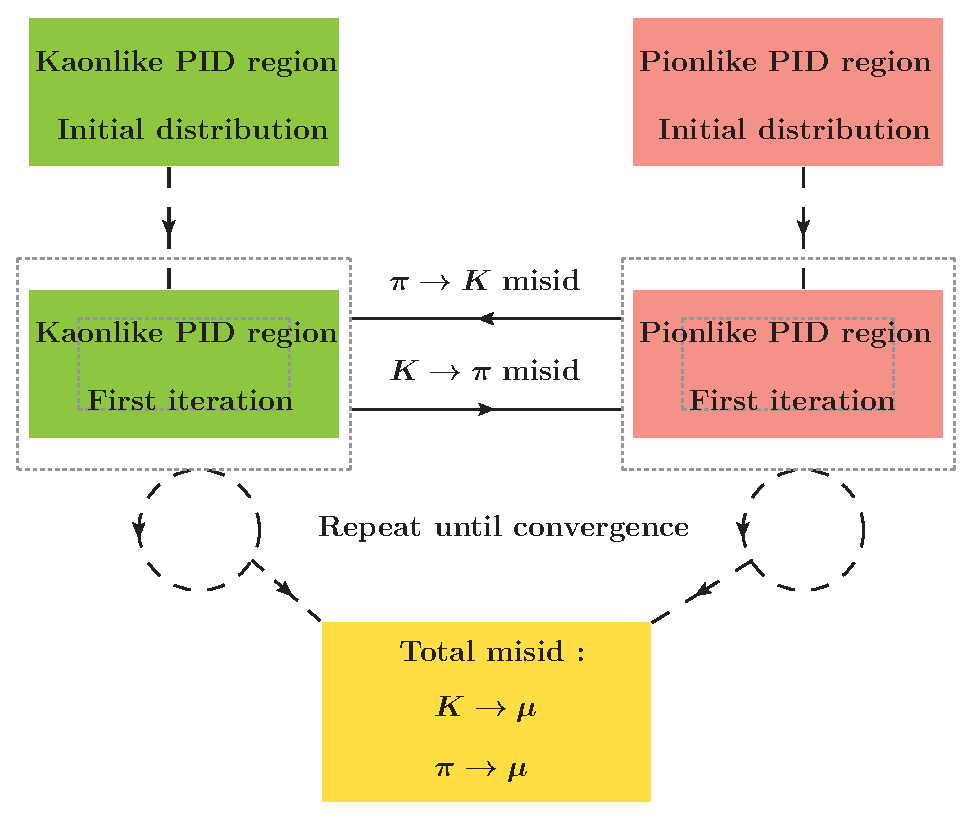
\includegraphics[width=0.6\linewidth]{bkg/misid/misid_att_3}%\put(-32,133){(a)}
    \vspace*{-0.5cm}
  \end{center}
  \caption{
    Diagram of the iterative procedure to establish contamination from decays where \DIFdelbeginFL \DIFdelFL{pion }\DIFdelendFL \DIFaddbeginFL \DIFaddFL{pions }\DIFaddendFL and \DIFdelbeginFL \DIFdelFL{kaon }\DIFdelendFL \DIFaddbeginFL \DIFaddFL{kaons }\DIFaddendFL are misidentified \DIFdelbeginFL \DIFdelFL{for muon}\DIFdelendFL \DIFaddbeginFL \DIFaddFL{as muons}\DIFaddendFL .
    }
  \label{fig:misidproc}
\end{figure}



Once the cross-feed between the different hadron species has been taken into account, the final step is to calculate the probability for
a specific hadron to pass the stringent muon \gls{PID} requirements applied in the analysis. The presence of the two real muons in the $\mumu h X$
background increases the probability to misidentify the hadron as a muon, mainly due to sharing of hits in the muon stations. Therefore the hadron misID probability is obtained from a dedicated control sample designed to emulate the topology of the mis-identified background,
 $B^{0} \rightarrow J/\psi(\rightarrow \mu^{+} \mu^{-}) K^{*}(\rightarrow \underline{K^{+} \pi^{-}})$, as shown in~\autoref{ratiatkos}.

%To determine the amount and the shape of the misID background data sample, same selection as for the signal sample is applied apart from \texttt{no \gls{PID} cut} on one muon, either positive or negative. The stripping selection for this sample is similar but with \texttt{no \gls{PID} cut} for the misidentified muon (SS or OS), see~\autoref{tab:misidbackground}.

This process can be summarized mathematically in \DIFdelbegin \DIFdel{a }\DIFdelend \DIFaddbegin \DIFadd{the }\DIFaddend following way:

\begin {itemize}
\item The proton-, pion- and kaon-like regions are defined in~\autoref{tab:misidregions}.

\begin{table}[ht]
\begin{center}
\begin{tabular}[t]{ l  l }
\toprule
Region & PID cuts  \\ \hline
	Proton-like & DLLp  > 5, DLLp - DLLK > 5 \\
Kaon-like & DLLK > 0, DLLp - DLLK < 5 \\
Pion-like & DLLK < 0, DLLp < 5 \\ \bottomrule
\end{tabular}
\end{center}
\caption{Species region definitions.}
\label{tab:misidregions}
\end{table}

%To estimate the shape of the background and size of it following procedure is applied:
%\begin {itemize}
%\item Subdivide
\item ID efficiencies are obtained from \texttt{PIDCalib} in bins of $p$, $\eta$ for all three regions.
\item MisID efficiencies are obtained from the specific calibration sample with two other muons in the sample in bins of $p$, $\eta$.
%Basic misID efficiencies are obtained for following cuts: \texttt{Particle\_(IsMuon==1.0) \&\& (DLLmu > 0.0) \&\& ((DLLmu - DLLK) > 0.0) \&\& (nShared==0)} as these are applied in stripping and selection.
%\item Some of the entries in the tuples are outside of default bins of \texttt{PIDCalib}/Calibration samples. For events below $p<3\gevc$, these are not considered and cut out (in signal data this is done by requiring \texttt{isMuon}). For events $p>100\gevc$, the same id/misID probability as the last bin is assigned.
%\item Some bins of \texttt{PIDCalib}/Calibration samples yield probabilities that are unphysical. These bins have either negative probabilities or probabilities above 1 (can arise due to $Splot$ technique used in \texttt{PIDCalib}). For bins with negative probabilities, probability is set to 0.00001. For bins with probability above 1 are set 1. And for bins which were not populated, the value from neighbouring bin was used. Remark: negative bins only appear for proton misID. As it will be shown in the misID fit section there is very small contribution from protons so there is no bias for the pion/kaon samples. The misID probabilities for different years will be discussed and shown in~\autoref{fig:JpsiKstWeights} and as it can be seen there are no negative bins.
\item In order to account for cross-contamination between the kaon and pions species the following procedure is applied:

 \begin{itemize} 

\item The data in each region is binned to obtain two dimensional $N(p, \eta)$ distributions\DIFdelbegin \DIFdel{, where $p$ is momentum and $\eta$ is pseudorapidity}\DIFdelend . The true \DIFdelbegin \DIFdel{kinematical }\DIFdelend \DIFaddbegin \DIFadd{kinematic }\DIFaddend distributions for kaons and pions are given by
\begin{equation}
n(p, \eta )^{0}_{\pi/K} = \frac{N(p, \eta )_{\pi/K}}{\epsilon(p,\eta )_{\pi/K}}.
\end{equation}
where $\epsilon(p,\eta)_{\pi/K}$ are efficiencies obtained from \texttt{PIDCalib} tables.

\item To correct for the cross-feed between \DIFaddbegin \DIFadd{the }\DIFaddend pion and kaon regions, the following algorithm which corrects the original distribution is applied:

\begin{equation}
n(p, \eta)^{i+1}_{\pi}=\frac{N(p, \eta)_{\pi}-M(p, \eta)_{K \rightarrow \pi} n(p, \eta)^{i}_{K}}{\epsilon(p,\eta)_{\pi}},
\end{equation}
\begin{equation}
n(p, \eta)^{i+1}_{K}=\frac{N(p, \eta)_{K}-M(p, \eta)_{\pi \rightarrow K} n(p, \eta)^{i}_{\pi}}{\epsilon(p,\eta)_{K}}.
\end{equation}

Here, $n(p, \eta)^{i}_{\pi}$  $n(p, \eta)^{i}_{K}$ together with the misID binned efficiencies $M(p, \eta )_{K \rightarrow \pi}$ and $M(p, \eta)_{\pi \rightarrow K}$ are estimating the-cross contamination between two regions. \DIFaddbegin \DIFadd{These ${K \rightarrow \pi}$ and ${\pi \rightarrow K}$ misID efficiencies are taken from }\texttt{\DIFadd{PIDCalib}}\DIFadd{.
}\DIFaddend 

%\item The next order distributions $n(p, \eta)^{i+1}_{\pi/K}$ are obtained by correcting the original distributions with the cross-contamination and then correcting for the ID binned efficiency.

\item At each iteration, the total number of misID particles of the type $\pi \rightarrow \mu$ and $K \rightarrow \mu$ \DIFdelbegin \DIFdel{events }\DIFdelend are given by
\begin{equation}
\sum_{p,\eta} n(p, \eta)^{i}_{\pi} M(p, \eta)_{\pi\rightarrow\mu} 
\end{equation}
\begin{equation}
\sum_{p,\eta} n(p, \eta)^{i}_{K} M(p, \eta)_{K\rightarrow\mu}
\end{equation}
\item This procedure is repeated until the change in total misID between iterations is less than 0.1\%. The typical number of iterations depends on the size of the sample. For big samples the convergence is achieved after two or three iterations. For small samples this is achieved after six iterations on average.

\item For each event in both the pion-like and the kaon-like sample, $w_{cross-feed}$ = probability of \DIFdelbegin \DIFdel{being misidentified particle }\DIFdelend \DIFaddbegin \DIFadd{a particle being misidentified }\DIFaddend including the cross-contamination correction, is 
	calculated as
\begin{equation}
	w^{\pi}_{cross-feed}=\frac{n(p, \eta)^{final}_{\pi} \times M(p, \eta)_{\pi\rightarrow\mu}}{{N(p, \eta)}^{0}_{\pi}},
\end{equation}
\begin{equation}
	w^{K}_{cross-feed}=\frac{n(p, \eta)^{final}_{K} \times M(p, \eta)_{K\rightarrow\mu}}{{N(p, \eta)}^{0}_{K}}.
\end{equation}
 \end{itemize} 

\item The number of misidentified events and the shape are obtained by reweighting the pion-like and kaon-like datasets by $w_{cross-feed}$. 

%	The difference between unweighted, weighted by PID efficiencies with no cross-feed, and weighted with cross-feed distributions can be seen in~\autoref{fig:misidtemp}.
 \end{itemize} 

Examples of misID distributions with unweighted, weighted by probability with no cross-feed correction, and weighted with cross-feed correction can be seen in~\autoref{fig:misidtemp} for the \textit{SS misID} and ~\autoref{fig:misidtempOS} for the \textit{OS misID}. These are the misID distributions before misid BDTs are applied, which minimize the contamination of this background as discussed in~\autoref{misidbdt}. 

\begin{figure}[H]
\center
\includegraphics[width = 0.9\textwidth]{/bkg/misid/example/compare_misid_modifiedandcutnSharednewData_B23MuNu_MisidSS_Run1_mu3isNotMuon_mu3inMuonAcc_trigger_Jpsi_mu1nShared_mu2nShared_qmincut_KaonPID__NEW.pdf}\put(-300,133){(a)}\put(-50,133){(b)}
\newline
\includegraphics[width = 0.9\textwidth]{/bkg/misid/example/compare_misid_modifiedandcutnSharednewData_B23MuNu_MisidSS_Run1_mu3isNotMuon_mu3inMuonAcc_trigger_Jpsi_mu1nShared_mu2nShared_qmincut_PionPID__NEW.pdf}\put(-300,133){(c)}\put(-50,133){(d)}
%\newline
%\includegraphics[width = 0.9\textwidth]{/bkg/misid/example/compare_misid_modifiedandcutnSharednewData_B23MuNu_MisidOS_Run1_mu2isNotMuon_mu2inMuonAcc_trigger_mu1nShared_mu3nShared_qmincut_KaonPID__NEW.pdf}\put(-300,133){(e)}\put(-50,133){(f)}
%\newline
%\includegraphics[width = 0.9\textwidth]{/bkg/misid/example/compare_misid_modifiedandcutnSharednewData_B23MuNu_MisidOS_Run1_mu2isNotMuon_mu2inMuonAcc_trigger_mu1nShared_mu3nShared_qmincut_PionPID__NEW.pdf}\put(-300,133){(g)}\put(-50,133){(h)}
\caption{Examples of \DIFaddbeginFL \DIFaddFL{the data }\DIFaddendFL distributions where the misID procedure is applied to obtain yields and shapes for Run \Rn{1}\DIFdelbeginFL \DIFdelFL{before misid BDT was applied}\DIFdelendFL . On the left, unweighted misID distributions (black), weighted with no cross-feed misID distributions (blue) and weighted misID distributions with cross-feed (red) for (a) kaon SS (c) pion SS . On the right, only weighted misID distributions for Run \Rn{1} (b) kaon SS (d) pion SS are shown together with the yield estimates. These shapes are obtained after the combinatorial BDT was applied, but before \DIFaddbeginFL \DIFaddFL{the }\DIFaddendFL misid BDT was applied. Total yields need to be multiplied by 100 to counteract the prescale that was applied on this data.}
\label{fig:misidtemp}
\end{figure}

\DIFaddbegin \DIFadd{This parametrisation of misID background is crucial for the final fit model described in~}\autoref{misidfitstrat}\DIFadd{.
}



\DIFaddend \begin{figure}[H]
\center
%\includegraphics[width = 0.9\textwidth]{/bkg/misid/example/compare_misid_modifiedandcutnSharednewData_B23MuNu_MisidSS_Run1_mu3isNotMuon_mu3inMuonAcc_trigger_Jpsi_mu1nShared_mu2nShared_qmincut_KaonPID__NEW.pdf}\put(-300,133){(a)}\put(-50,133){(b)}
%\newline
%\includegraphics[width = 0.9\textwidth]{/bkg/misid/example/compare_misid_modifiedandcutnSharednewData_B23MuNu_MisidSS_Run1_mu3isNotMuon_mu3inMuonAcc_trigger_Jpsi_mu1nShared_mu2nShared_qmincut_PionPID__NEW.pdf}\put(-300,133){(c)}\put(-50,133){(d)}
%\newline
\includegraphics[width = 0.9\textwidth]{/bkg/misid/example/compare_misid_modifiedandcutnSharednewData_B23MuNu_MisidOS_Run1_mu2isNotMuon_mu2inMuonAcc_trigger_mu1nShared_mu3nShared_qmincut_KaonPID__NEW.pdf}\put(-300,133){(a)}\put(-50,133){(b)}
\newline
\includegraphics[width = 0.9\textwidth]{/bkg/misid/example/compare_misid_modifiedandcutnSharednewData_B23MuNu_MisidOS_Run1_mu2isNotMuon_mu2inMuonAcc_trigger_mu1nShared_mu3nShared_qmincut_PionPID__NEW.pdf}\put(-300,133){(c)}\put(-50,133){(d)}
\caption{Examples of \DIFaddbeginFL \DIFaddFL{data }\DIFaddendFL distributions where \DIFaddbeginFL \DIFaddFL{the }\DIFaddendFL misID procedure is applied to obtain yields and shapes for Run \Rn{1}\DIFdelbeginFL \DIFdelFL{before misid BDT was applied}\DIFdelendFL . On the left, unweighted misID distributions (black), weighted with no cross-feed misID distributions (blue) and weighted misID distributions with cross-feed (red) for (a) kaon OS (c) pion OS. On the right, only weighted misID distributions for Run \Rn{1} (b) kaon OS (d) pion 0S are shown together with the yield estimates.  These shapes are obtained after \DIFaddbeginFL \DIFaddFL{the }\DIFaddendFL combinatorial BDT was applied, but before \DIFaddbeginFL \DIFaddFL{the }\DIFaddendFL misid BDT was applied. Total yields need to be multiplied by 100 to counteract the prescale that was applied on this data.}
\label{fig:misidtempOS}
\end{figure}


\section{Partially Reconstructed Background}
\label{partrecobak}
Partially reconstructed background can occur by missing or misidentifying one or more particle tracks in the decay. The common feature for this type of \DIFdelbegin \DIFdel{backgrounds }\DIFdelend \DIFaddbegin \DIFadd{background }\DIFaddend is that the corrected or reconstructed mass of the $B$ will be lower than in the signal case.

In order to estimate both the shape and the size of the partially reconstructed \DIFdelbegin \DIFdel{backgrounds}\DIFdelend \DIFaddbegin \DIFadd{background}\DIFaddend , one of the most dangerous \DIFdelbegin \DIFdel{example }\DIFdelend \DIFaddbegin \DIFadd{examples }\DIFaddend is studied: $B^+ \rightarrow (D^0 \rightarrow K^- \pi^+ \mu^{+} \mu^{-})\mu \nu$. The expected $\mathcal{B}(\pr)$ is obtained by multiplying $\mathcal{B}(D^{0} \rightarrow K^+ \pi^- \mu^+ \mu^{-}) = (4.17\pm0.12\pm0.40)\times 10^{-6}$\cite{Aaij:2015hva} and $\mathcal{B}(B^{+} \rightarrow D l^{+} \nu X) = (9.8 \pm 0.7)\times 10^{-2}$ \cite{Patrignani:2016xqp} yielding $\mathcal{B}(\pr) \approx (4.1\pm0.5)\times 10 ^{-7}$.

The shape of this background is investigated with inclusive simulation samples containing also higher excited resonances $D^{*0}, D_{2}^{*0}$, and so on. As this sample was simulated for a different analysis, it has one imperfection: it has two charged pions rather than muons coming from the $D^{0}$ decay, which are reconstructed as signal. In this study the effect of missing particles on the corrected mass shape is investigated hence these two pions become good proxies for the muons given the muon and pion have very similar mass. The only problem that could arise is if the selection efficiency was not constant as a function of the dipion mass, $M(\pi^{+}\pi^{-})$, as this would lead to shaping of the background, potentially underestimating the contributions from the resonant $\omega$ and $\rho$ region, which are present with the two muons. 

For this reason all muon cuts from the selection apart from the \gls{PID} are also applied to the pions. Relative efficiency ratios including all the efficiencies after the MVA stage are obtained, where for signal the total selection efficiency is $\varepsilon^{total}_{\Bmumumu}=(2.63 \pm 0.03)\times 10^{-3}$ and for \DIFaddbegin \DIFadd{the }\DIFaddend partially reconstructed background $\varepsilon^{total}_{\pr}=(6.82 \pm 0.07)\times 10^{-4}$. Assuming the branching fractions for $\mathcal{B}(\Bmumumu) = 1\times10^{-8}$ and for $\mathcal{B}(\pr ) = (4.1\pm0.5)\times10^{-7}$, the relative contamination between signal and partially reconstructed background results in~\autoref{fig:expectedinter}(a). 

To check the fact that there is no dangerous shaping of the background using this particular proxy simulation sample, the full selection efficiency in bins of dipion mass is plotted. The \DIFdelbegin \DIFdel{efficiency flatness }\DIFdelend \DIFaddbegin \DIFadd{flat efficiency }\DIFaddend shown in~\autoref{fig:expectedinter}(b) means that this selection does not have model dependence and hence it is safe to use for shape estimates for the partially reconstructed backgrounds.
%not exact because of minq contamination

\begin{figure}[H]
\centering
\includegraphics[width = 0.5\textwidth]{bkg/pr/variableBplus_Corrected_MassPartRecoScaled2012_0_102_supernice.pdf}\put(-50,70){(a)}
\includegraphics[width = 0.47\textwidth]{bkg/pr/SelectionEfficiency_invmu1andmu2_PARTRECOMC_special.pdf}\put(-50,70){(b)}
	\caption{(a) Signal and partially reconstructed background distributions scaled to their expected ratio after \DIFaddbeginFL \DIFaddFL{the }\DIFaddendFL full MVA selection assuming \DIFaddbeginFL \DIFaddFL{the }\DIFaddendFL following branching fractions: $\mathcal{B}(\Bmumumu ) = 1\times10^{-8}$ and $\mathcal{B}(\pr ) = (4.1\pm0.5)\times10^{-7}$. (b) Full selection efficiency as a function of invariant mass of the proxy pions is constant.}
\label{fig:expectedinter}
\end{figure}


The most powerful part of the selection that eliminates this \DIFdelbegin \DIFdel{part of the }\DIFdelend background is isolation as partially reconstructed background \DIFdelbegin \DIFdel{decay had usually has }\DIFdelend \DIFaddbegin \DIFadd{decays usually have }\DIFaddend more tracks. In order to \DIFdelbegin \DIFdel{estimated }\DIFdelend \DIFaddbegin \DIFadd{estimate the }\DIFaddend contamination in the final fit, normalisation with respect to \bjpsimumuk is used as shown in~\autoref{finfitpr}.

\subsection{Partially Reconstructed Backgrounds, where \mb{D^{0} \rightarrow \eta / \eta' X}, and \mb{\eta / \eta' \rightarrow \mu \mu \gamma}}
\label{etasec}
In the previous partially reconstructed sample, the background that \DIFdelbegin \DIFdel{proceed }\DIFdelend \DIFaddbegin \DIFadd{proceeds }\DIFaddend via $\eta/\eta'$ from a $D$ decay is not considered, as it is not part of the inclusive simulation. The selection efficiency of such decays is expected to \DIFdelbegin \DIFdel{have very similar values as in }\DIFdelend \DIFaddbegin \DIFadd{be very similar to }\DIFaddend the partially reconstructed sample proxy, because the reconstructed particles are the same.

In this section, the total estimate for the branching fraction of the partially reconstructed backgrounds proceeding via $\eta/\eta'$ from $D$ decays is computed. The full inclusive rate $\mathcal{B} (D^{0} \rightarrow \eta / \eta' X)$ is $ \sim 10 \%)$. However, the most relevant decay chains are the ones where the mass of the missed particle(s) is small. This is because if only a light particle is missed, the shape of the corrected mass of partially reconstructed background comes closest to the signal region. Such decay chains are considered in~\autoref{tab:etacont}.

It can be seen that the total cumulative contribution is much smaller then the one considered with $D^{0}\rightarrow K^{+} \pi^{-} \mu^{+} \mu^{-}$, where $\mathcal{B}(D^0 \rightarrow K \pi^+ \mu^{+} \mu^{-}) = (4.17\pm0.12 \rm{(stat)}\pm 0.40 \rm{(syst)})\times 10^{-6}$\cite{Aaij:2015hva}. No further consideration hence is necessary for this type of decay.

\begin{table}[ht]
\begin{center}
\begin{tabular}{ l  c  c }

\toprule
	Process & $\mathcal{B}$ & Contribution to $\mathcal{B}(D^{0} \rightarrow (\eta / \eta'\rightarrow \mu \mu \gamma) X)$ \\
\hline

$\mathcal{B}(\eta \rightarrow \mu \mu \gamma)$ & $(3.10\pm0.40)\times 10 ^{-4 }$ & -  \\
$\mathcal{B}(\eta' \rightarrow \mu \mu \gamma)$ & $(1.08\pm0.27)\times 10 ^{-4 }$ & -  \\
\hline
$\mathcal{B}(D^{0} \rightarrow \eta' \pi^{0})$ & $(9.10\pm1.40)\times 10 ^{-4 }$ & $(9.80\pm2.90)\times 10 ^{-8 }$ \\
$\mathcal{B}(D^{0} \rightarrow \eta' \pi^{+} \pi^{-})$ & $(4.50\pm1.70)\times 10 ^{-4 }$ & $(4.90\pm2.20)\times 10 ^{-8 }$ \\
$\mathcal{B}(D^{0} \rightarrow 2\eta )$ & $(1.70\pm0.02)\times 10 ^{-3 }$ & $(5.30\pm0.70)\times 10 ^{-7 }$ \\
$\mathcal{B}(D^{0} \rightarrow 2\eta )$ & $(1.70\pm0.02)\times 10 ^{-3 }$ & $(5.30\pm0.70)\times 10 ^{-7 }$ \\
$\mathcal{B}(D^{0} \rightarrow \underline{\eta} \eta' )$ & $(1.06\pm0.27)\times 10 ^{-3 }$ & $(3.30\pm0.90)\times 10 ^{-7 }$ \\
$\mathcal{B}(D^{0} \rightarrow \eta \underline{\eta}' )$ & $(1.06\pm0.27)\times 10 ^{-3 }$ & $(1.10\pm0.40)\times 10 ^{-7 }$ \\
$\mathcal{B}(D^{0} \rightarrow \eta \phi)$ & $(1.40\pm0.50)\times 10 ^{-4 }$ & $(4.30\pm1.60)\times 10 ^{-8 }$ \\
\hline
Total &  - &$(1.69\pm0.15)\times 10 ^{-6 }$ \\
\bottomrule
\end{tabular}
\end{center}
\caption{Contribution to total $D^{0} \rightarrow (\eta / \eta'\rightarrow \mu \mu \gamma) X$ rate made from all the \DIFdelbeginFL \DIFdelFL{considered }\DIFdelendFL decays \DIFaddbeginFL \DIFaddFL{considered }\DIFaddendFL above. In total, this cumulative contribution is approximately three times smaller than $D^{0}\rightarrow K^{+} \pi^{-} \mu^{+} \mu^{-}$. All the branching fractions are obtained from \cite{Patrignani:2016xqp}.}
\label{tab:etacont}
\end{table}

\subsection{Partially Reconstructed \mb{B \rightarrow \eta (') V} Backgrounds}
The backgrounds with $\eta(')$ resonances from partially reconstructed decays that proceed via $D$ decays were considered in\DIFdelbegin \DIFdel{previous}\DIFdelend ~\autoref{etasec}. In this section backgrounds with $\eta(')$ along with vector resonances $\omega$/$\rho$ coming directly from \DIFaddbegin \DIFadd{the }\DIFaddend $B$ are estimated. The total branching fractions for these processes are listed in~\autoref{tab:ed} and since they are very small this type of background is discarded and will not be considered further.

\begin{table}[ht]
\begin{center}
\begin{tabular}{ l  c }
\toprule
Process & $\mathcal{B}$  \\
\hline
$\mathcal{B}(B^{0} \rightarrow \omega \eta')$ & $(1.00\pm0.50)\times 10 ^{-6 }$ \\
$\mathcal{B}(B^{0} \rightarrow \rho \eta')$ &  $<$$5 \times 10 ^{-7}$  \\
$\mathcal{B}(B^{0} \rightarrow  \omega  \eta )$ & $(9.00\pm4.00)\times 10 ^{-7 }$ \\
$\mathcal{B}(B^{0} \rightarrow \rho \eta )$ & $<$ $5 \times 10 ^{-7}$   \\
\hline
$\mathcal{B}(\eta \rightarrow \mu \mu \gamma)$ & $(3.10\pm0.40)\times 10 ^{-4 }$ \\
$\mathcal{B}(\eta' \rightarrow \mu \mu \gamma)$ & $(1.08\pm0.27)\times 10 ^{-4 }$  \\
\hline
$\mathcal{B}(\rho \rightarrow \mu \mu)$ & $(4.55\pm0.28)\times 10 ^{-5 }$  \\
$\mathcal{B}(\omega \rightarrow \mu \mu)$ & $(9.00\pm3.10)\times 10 ^{-5 }$  \\
\hline
Process & Contribution to $B^{0} \rightarrow (\eta(')\rightarrow \mu \mu \gamma) (\rho(\omega)\rightarrow \mu \mu)$ \\
\hline
$\mathcal{B}(B^{0} \rightarrow (\omega \rightarrow \mu \mu) (\eta \rightarrow \mu \mu \gamma))$ &$(7.10\pm1.00)\times 10 ^{-15 }$ \\
$\mathcal{B}(B^{0} \rightarrow (\omega \rightarrow \mu \mu) (\eta'\rightarrow \mu \mu \gamma))$ &$(2.50\pm0.60)\times 10 ^{-15 }$ \\
$\mathcal{B}(B^{0} \rightarrow (\rho \rightarrow \mu \mu) (\eta \rightarrow \mu \mu \gamma))$ & $<$$(2.50\pm1.40)\times 10 ^{-14 }$ \\
$\mathcal{B}(B^{0} \rightarrow (\rho \rightarrow \mu \mu) (\eta'\rightarrow \mu \mu \gamma))$ & $<$$(1.00\pm0.60)\times 10 ^{-14 }$ \\
\hline
Total  & $ <$ $(4.50\pm1.60)\times 10 ^{-14 }$ \\
\bottomrule
\end{tabular}
\end{center}
\caption{Different and total contribution to $B^{0} \rightarrow \eta(') \rho(\omega)$. All the branching fractions are obtained from \cite{Patrignani:2016xqp}.}
\label{tab:ed}
\end{table}


\section{Rare and Resonant \mb{B^{+} \rightarrow \pi^{+} / K^{+} \mu^{-} \mu^{+}} Backgrounds}
\label{rareandreso}
The resonant backgrounds arising through $B^{+} \rightarrow (J/\psi \rightarrow \mu^{-} \mu^{+}) X^{+}$ and $B^{+} \rightarrow (\psi(2S) \rightarrow \mu^{-} \mu^{+}) X^{+}$ decay chains are eliminated because of the $c\bar{c}$ veto as discussed in~\autoref{qsqchoice}.

It is, however, necessary to evaluate the impact of the rare equivalent of this background, namely \bmumupi decays, where the $\pi^{+}$ is misidentified as muon. The $\mathcal{B}(\bmumupi)=1.79\pm0.23\times 10^{-8}$\cite{Patrignani:2016xqp}. The contribution of this background is accounted for in\DIFdelbegin \DIFdel{the}\DIFdelend ~\autoref{misidprocedure}, but it is crosschecked as this particular background peaks just under the corrected mass of \DIFaddbegin \DIFadd{the }\DIFaddend $B$. For the same rare decay but with a kaon instead, \bmumuk, the mass is expected to be shifted away from this peak because of the higher kaon mass.

In order to establish the severity of this background, the \bmumupi simulation for Run \Rn{1} and 2016 is reconstructed where the muon mass hypothesis is used for the pion track candidate. %This means that energy of this candidate is recalculated. 
Afterwards the same selection as in the signal case is applied. The expected number of \bmumupi decays after the full selection in a given Run can be calculated by normalising to \bjpsimumuk decays. In the end 0.06 (0.03) \bmumupi events are expected in Run \Rn{1} (2016) which is negligible given that there are $\sim$ 17 expected signal events with $\mathcal{B}(\Bmumumu)=1\times 10^{-8}$. Hence no further specific action for this background is taken, however, its contribution is directly accounted for in\DIFdelbegin \DIFdel{the}\DIFdelend ~\autoref{misidprocedure}.

%\begin{equation}
%	N(\bmumupi)= \frac{N(\bjpsimumuk)}{} \times \frac{\varepsilon^{total}_{\bmumupi}}{\varepsilon^{total}_{\bjpsimumuk}} \times \frac{\mathcal{B}(\bmumupi)}{\mathcal{B}(\bjpsimumuk)}.
%\end{equation}

%info foun in /vols/lhcb/ss4314/final_tuples_analyser_PO_AND_UE/mc/pimumu_mc/normalize_to_jpsik/bin
%why reco factor of 100?


%In this equation the following branching fractions are used: $\mathcal{B}(\bmumupi)=1.79\pm0.23\times 10^{-8}$\cite{Patrignani:2016xqp} and $\mathcal{B}(\bjpsimumuk)=(6.12\pm0.19)\times10^{-5}$) obtained by multiplying $\mathcal{B}(B^{+} \rightarrow J/\psi K^{+}) = (1.026\pm 0.031)\times 10^{-3}$\cite{Patrignani:2016xqp} and $\mathcal{B}(J/\psi \rightarrow \mu^{-} \mu^{+}) = (5.961 \pm0.003) \times 10^{-2}$\cite{Patrignani:2016xqp}. The total selection efficiencies without \gls{PID} are $\varepsilon^{total}_{\bmumupi}=(7.03 \pm 1.13)\times 10^{-6}$ and $\varepsilon^{total}_{\bjpsimumuk}=(5.8\pm0.01)\times10^{-3}$ where the reconstruction and combinatorial BDT efficiency is much lower for the \bmumupi mode. Using the yields obtained in~\autoref{tab:normchannelyields} 0.06 (0.03) \bmumupi events are expected in Run \Rn{1} (\Rn{2}) which is negligible given that there are $\sim$ 17 expected signal events with $\mathcal{B}(\Bmumumu)=1\times 10^{-8}$. Hence no further specific action for this background is taken, however, its contribution is directly accounted for in the~\autoref{misidprocedure}.

\section{Summary}
In conclusion, different backgrounds that can mimic the signal were studied. From all \DIFdelbegin \DIFdel{considered backgrounds only }\DIFdelend \DIFaddbegin \DIFadd{backgrounds considered only the }\DIFaddend combinatorial, misID and partially reconstructed backgrounds have considerable contribution after all the \DIFdelbegin \DIFdel{selection }\DIFdelend \DIFaddbegin \DIFadd{selections }\DIFaddend and hence need to be modelled. \DIFdelbegin \DIFdel{Exact }\DIFdelend \DIFaddbegin \DIFadd{The exact }\DIFaddend contribution of these three backgrounds is discussed in~\autoref{sigpara}.


\input{Efficiency_corrected}
%% %%%%%%%%%%%%%%%%%%%%%%%%%%%%%%%%%%%%%%%%%%%%%%%%%%%%%%%%%%%%%%%%%%%%%%%%%%%%%%%%%%
\chapter{Multivariate methods used in the $\mathbold{\Lbpi}$ analysis}
\label{chap:bdt}
This chapter will outline the multivariate analysis (MVA) methods used in the \Lbpi analysis to reduce background. The MVA methods used in this analysis are in the form of BDTs, which are trained and implemented using a dedicated MVA software package \cite{TMVA}. A brief overview of MVA methods using BDTs can be found in Appendix \ref{app:bdt}. There are two BDTs used in this analysis. The first BDT, referred to as the isolation BDT, is designed to determine how isolated the final state tracks of the signal channel are, and is discussed in detail in~\autoref{sec:iso}. The isolation BDT output is then taken as an input for the BDT used to reduce combinatorial background, discussed in~\autoref{Sec:BDT}. The optimisation process for the cut placed on the combinatorial BDT output is discussed in~\autoref{sec:opt}.

\section{Isolation of the final state tracks}
\label{sec:iso}
The isolation BDT used in this analysis was originally trained for the analysis in Ref\cite{LHCB-ANA-2014-048}. The algorithm used iterates over every track in an event which is not a candidate signal track, as illustrated in~\autoref{Fig:iso}, where the non-signal candidate track is denoted $i$. The BDT algorithm then computes how signal-like each track is, depending on the variables given in~\autoref{tab:iso}. In~\autoref{tab:iso}, the ghost probability (ghost prob.) is an estimate of the probability that a track is a so-called \gls{ghost} track. Such a track has less than 70\% of its hits originating from a single particle, where the number of hits is evaluated only from simulation. %of a track is the probability that at track is a so-called ghost track, where a ghost track is defined as being a track which has less than 70\% of the hits making up the track originating from the same track. 

 %The algorithm iterates over every track in an event which is not a candidate signal track, as illustrated in~\autoref{Fig:iso}, and computes how signal-like each track is, depending on the variables given in~\autoref{tab:iso}. 
\begin{figure}[ht!]
    \centering
  \includegraphics[scale = 0.3, trim = 0.5cm 0cm 0cm 0cm, clip]{figs/isolation1.png}
  \caption{A schematic of a non-signal track, $i$, and a \Lbpi candidate.}
    \label{Fig:iso}
\end{figure}


\begin{table}[h!]
  %\hline
  
  \centering
  \begin{tabular}{c}

    \hline
    Variables used in the isolation BDT\\
    \hline
    $\pt_{\mathrm{track}}$\\
    $\vec{p}_{\mathrm{track}}.\vec{p}_{\proton\pi\mu\mu}$\\ %%_{track},\p_{})\\
    $\mathrm{ghost}$ $\mathrm{prob.}_{\mathrm{track}}$\\
    $\chi^{2}_{\mathrm{track}}$ \\
    $IP{\chi^{2}}_{\mathrm{track}}$ ($\proton\pi\mu\mu$ vertex)\\
    \hline
  \end{tabular}
  \caption{The variables used in the isolation BDT.}
  \label{tab:iso}
\end{table}

%\subsection{Signal and background training samples}
In Ref\cite{LHCB-ANA-2014-048}, the isolation BDT was trained using $\Lb\to\proton\mun\nu$ simulation as the signal proxy and $\Lb\to(\Lc\to \proton X\mun\nu)\mun\nu$ as the background proxy. The resulting BDT weights, which were not obtained by myself but simply taken the analysis in \cite{LHCB-ANA-2014-048}, were then applied to this analysis. Although the training samples differ in many aspects from \Lbpi, the variables used in the training, as shown in~\autoref{tab:iso}, are generic enough such that the resulting BDT can be applied to a range of channels. The BDT weights for the isolation BDT are computed prior to any selection.%The response, as shown in~\autoref{Fig:isow}, is still very discriminating,~\autoref{Fig:isow} shows the isolation BDT response for \LbKjpsi data, representing the signal proxy, and the response for the upper mass side band of \Lbpi data, representing the background.
\subsection{Isolation BDT response}
The isolation BDT output of the non-candidate track which is most signal-like is used as the nominal isolation BDT output value. The output of the isolation BDT applied to sWeighted \LbKjpsi data (signal) and \Lbpi candidates with a mass above 6000\mevcc (background), is shown in~\autoref{Fig:isow}.
\begin{figure}[ht!]
    \centering
  \includegraphics[height = 5.5cm, trim = 0cm 0cm 0cm 0cm, clip]{figs/isolationoutput}
  \caption{The isolation BDT response for \LbKjpsi data, representing the signal proxy, and the response for the upper mass side band of \Lbpi data, representing the background.}
    \label{Fig:isow}
\end{figure}
The peak in the signal output at -2 corresponds to cases where no non-signal track in the event passes the preselection applied, so the signal candidates are completely isolated. %The output for this isolation BDT in used as an input variable for the combinatorial BDT.
%%%%%%%%%%%%%%%%%%%%%%%%%%%%%%%%%%%%%%%%%%%%%%%%%%%%%%%%%%%%%%%%%%%%%%%%%%%%%%%%%%
\section{The combinatorial Boosted Decision Tree}
\label{Sec:BDT}
In order to reduce combinatorial and reflection background, a further BDT is trained using \Lbpi data above 6000\mevcc as a proxy for the combinatorial background and sWeighted \LbKjpsi data as a proxy for the signal events.
%% The training options can be seen in~\autoref{tab:bdtchoice}.
%% \begin{table}
%%   \centering
%%   \begin{tabular}{ c }
%%     \hline
%%     Variable & Choice \\
%%     \hline
%%     NTrees&200\\
%%     nCuts&-1\\
%%     MinNodeSize&3\\
%%     MaxDepth&3\\
%%     SeparationType&Gini Index\\
%%     PruneMethod& No pruning\\
%%     \hline
%%   \end{tabular}
%%   \caption{Training options used in the BDT. These variables are defined in Ref\cite{cmsada}.}
%%   \label{tab:bdtchoice}
%% \end{table}
To choose which variables were used as inputs to the BDT, a large range of variables were initially selected and those that were deemed least discriminating, based on how often the variables were used to split a tree and the size of the separation resulting from such a split, were disregarded. The final selection of variables, ordered by separation power, is shown in~\autoref{tab:bdtvars}. The $N^{*}$ in~\autoref{tab:bdtvars} refers to the combination of the $\proton\pi$ as if they came from a $N^{*}$ decay, $\Lb\to N^{*}(\to\proton\pim)\mup\mun$. Variables that assume that the $\proton\pi$  come from an $N^{*}$ are used because much of the signal will genuinely decay via this resonance, whereas this is not the case in combinatorial background. The $\mup$ \dllmupi refers to whichever muon has the same sign as the proton, so in the conjugate case this would be $\mun$. The difference in separation power amongst the weakest eight BDT variables is minimal. The $\mup$ \dllmupi is slightly more discriminating than the equivalent $\mun$ \dllmupi variable, and therefore only the former was included as an input variable. This is thought to be due to the mis-identification of pions as muons in the combinatorial background coming from $\Lc$ decays. The DecayTreeFitter (\gls{DTF}) $\chi^{2}$ refers to the $\chi^{2}$ per degree of freedom of the simultaneous fit to the complete decay chain. The PID variables are used in the BDT in order to exploit the varying PID performance with kinematics and thus help further reduce contributions from reflection backgrounds. %This means that there are two possible proxies, resampled simulation or a suitable channel selected from the data.

The distribution of the input variables for the signal and background training samples are shown in Figures \ref{Fig:bdtvar1}, \ref{Fig:bdtvar2} and \ref{Fig:bdtvar3}.
%An intial list of variables can be seen below in Figures~\ref{Fig:bdt1},~\ref{Fig:bdt2},~\ref{Fig:bdt3} with signal simulation in red and data falling above \Lb $>$ 6000\mevcc in black.
%\vspace*{-5cm}
\begin{table}[!ht]

  \centering
  \hspace*{-0.5cm}
  \begin{tabular}{|c|c|c|c|c|c|}
    \hline
    Rank& Variable& Seperation / 0.1 &Rank& Variable& Seperation / 0.1 \\\hline
    1&\Lb vertex \gls{bm}         &9.0     & 10&      $\pim$ \gls{ipchi2}    &0.7     \\
    2&$\Lambda_{b}$  \Gls{DIRA}   &3.4            & 11&  $\mup$ \dllmupi                  &0.6                  \\
    3&Isolation BDT output        &2.9                      & 12&                     $\proton$ \gls{ipchi2}&0.6\\
    4&$\Lambda_{b}$ $\tau$        &2.8          & 13&          $\proton$ IP                        &0.5 \\
    5&$\Lambda_{b}$ $\pt$         &2.4          & 14& $\proton$ \dllppi                            &0.4          \\
    6&$\Lambda_{b}$ DecayTreeFitter $\chi^{2}$ &1.8& 15& $\Lambda_{b}$ \gls{ipchi2}        & 0.3\\
    7&$N^{*}$ \gls{ipchi2}              &1.8 & 16&   $\proton$ \dllpk                       &0.1            \\
    8&$N^{*}$ $\pt$                     &1.6    & 17&     $\proton$ $|\vec{p}|$             &0.1              \\
    9&$\Lambda_{b}$ $|\vec{p}|$         &0.9    & & &\\
    \hline
  \end{tabular}

  \caption{List of BDT input variables. The variables are listed in order of their separation power. The seperation values are also listed.}
      \label{tab:bdtvars}
\end{table}
%\FloatBarrier

    \begin{figure}[!ht]\def\nh{0.6\textwidth}
  \centering
\hspace*{-2cm}
  \includegraphics[height=\nh]{figs/canvas1_var_edited.pdf}

  \caption{The first six variables used in the combinatorial BDT for signal and background proxies. The red stripped histograms are background and the solid blue histograms are signal. All distributions shown are normalised. The variable \Lb $\mathrm{EV}_{\chisq}$ refers to \Lb \gls{bm} in~\autoref{tab:bdtvars}.}
  \label{Fig:bdtvar1}
    \end{figure}
   
    \begin{figure}[!ht]\def\nh{0.6\textwidth}
  \centering
  \hspace*{-2cm}
  \includegraphics[height=\nh]{figs/canvas2_var_edited.pdf}

  \caption{The second six variables used in the combinatorial BDT for signal and background proxies. The red stripped histograms are background and the solid blue histograms are signal. All distributions shown are normalised.}
  \label{Fig:bdtvar2}
    \end{figure}
    \FloatBarrier
    \begin{figure}[!ht]\def\nh{0.65\textwidth}
  \centering
  \hspace*{-1cm}
  \includegraphics[scale = 0.9]{figs/canvas3_var_edited.pdf}

  \caption{The final five variables used in the combinatorial BDT for signal and background proxies. The red stripped histograms are background and the solid blue histograms are signal.  All distributions shown are normalised. The variable \Lb DTF \chisq refers to $\Lambda_{b}$ DecayTreeFitter $\chi^{2}$ in~\autoref{tab:bdtvars}. }
  
  \label{Fig:bdtvar3}
    \end{figure}
    \FloatBarrier
   
    The BDT is trained using the K-Folding technique \cite{kfold}: each event is randomly assigned an integer, $i$, between 0 and the number of K-Folds, $n$, (in this case $n$ = 5) and $n$ BDTs are trained with the $i^{th}$ BDT being tested on the $i^{th}$ data set and trained on the remaining data. Employing this technique allows ($n$-1)/$n$ of the data set to be used to train the BDT. 


%% As discussed in~\autoref{Sec:backgrounds}, for the normalisation (signal) channels, the largest reflection background comes from \BdToJPsiKst (\BdToKstmm) decays. These are distinguished from \Lbpijpsi (\Lbpi) decays through the PID variable $\dllpk$, meaning it is important to have this variable in the BDT. However, as discussed in~\autoref{Sec:Selection}, this PID variable is poorly modelled in resampled simulation. For this reason, sWeighted \LbKjpsi data is used a signal proxy rather than simulation.



\section{The BDT performance and optimisation}
\label{sec:opt}
The BDT response for each K-Fold, as well as the signal efficiency against background rejection, integrated over all K-Fold's, is shown in~\autoref{Fig:kfoldBDT}. The red line in~\autoref{Fig:kfoldBDT}\protect\subref{q2:6} indicates the BDTs optimal working point. The choice of working point is discussed later in this section.


%% 
\begin{figure}[!t]\def\nh{0.3\textwidth}
  \centering



  \subfloat[]{\includegraphics[height=\nh]{figs/RE_bdt1}\label{q2:1}} \hskip 0.04\textwidth
  \subfloat[]{\includegraphics[height=\nh]{figs/RE_bdt2}\label{q2:2}} \\
  \subfloat[]{\includegraphics[height=\nh]{figs/RE_bdt3}\label{q2:3}}\hskip 0.04\textwidth
    \subfloat[]{\includegraphics[height=\nh]{figs/RE_bdt4}\label{q2:4}} \\
  \subfloat[]{\includegraphics[height=\nh]{figs/RE_bdt5}\label{q2:5}} \hskip 0.04\textwidth
  \subfloat[]{\includegraphics[height=\nh]{figs/roc}\label{q2:6}}\\


 \caption{The BDT response for all 5 K-Folds and the signal efficiency against background rejection curve, integrated over all K-Folds. The red line on the signal efficiency against background rejection curve indicates the optimal working point.}
  \label{Fig:kfoldBDT}

\end{figure}


As there is no branching fraction prediction, the BDT is optimised using the Punzi \gls{FOM} \cite{Punzi:2003bu} defined as

\begin{equation}
  \mathrm{FOM}_{\mathrm{PUNZI}} = \frac{\epsilon_{\mathrm{selection}}}{\sigma/2  + \sqrt{B}},
  \label{eq:punz}
\end{equation}
where $\epsilon_{\mathrm{selection}}$ refers to the efficiency of the selection and $B$ refers to the number of background events.
The Punzi FOM is also a function of the target significance, $\sigma$. The target significance is 3$\sigma$. There is no change in the chosen working point if this is varied by $\pm0.5\sigma$. %varied between 2.5 $\sigma$ and 3.5$\sigma$ and there is found to be no change to the optimal working point due to this variation.

In order to deduce $B$, a fit is performed to the blinded mass spectrum of \Lbpi data. The blinded region in mass is taken as 5530$<m_{p\pi\mu\mu}<$5710 \mevcc, which removes all signal events according to simulation. The data is fitted either side of the blinded region and the number of background events is taken by extrapolating the background probability density function (PDF) across the blinded region. The details of the fit model used are discussed in~\autoref{chap:mass}.

As the number of background events across the signal window\
is very low ($\sim$ 5 or less for BDT cuts greater than $\sim$ 0.3), the FOM is calculated many times, each time randomly choosing a yield of background events within one standard deviation of the true value. This is done with the aim of reducing the sensitivity to the large uncertainty on the shape of the combinatorial background.

To obtain the value of $\epsilon_{\mathrm{selection}}$ in~\autoref{eq:punz}, the BDT efficiency is calculated using \LbKjpsi data, and is also compared to the efficiency derived from \LbK data. This BDT efficiency is then multiplied by the rest of the selection efficiency (see~\autoref{chap:mass}).
The BDT efficiency calculated with both \LbK and \LbKjpsi data as a function of BDT output value is shown in~\autoref{Fig:BDTeff}. To deduce the BDT efficiency, the yield extracted from the fit to \LbKjpsi data is compared to that extracted from a subsequent fit to \LbKjpsi data with the relevant BDT cut applied. In the case of \LbK data, the same method is used but a BDT cut of 0 is initially placed on the \LbK data, as without this cut the background to signal ratio is too large and the fit becomes difficult to perform.
\begin{figure}[!ht]
  \centering
  \includegraphics[height = 5.5cm]{figs/BDT_eff_jpsi_mumu_pk}
  \caption{The efficiency of the BDT as a function of BDT cut value using \LbK and \LbKjpsi sWeighted data. The dashed line shows the efficiency at the working point of 0.25.}
  \label{Fig:BDTeff}
\end{figure}

The values of the Punzi FOM as a function of the BDT cut value are shown in~\autoref{Fig:PUNZI}. Each line represents a different assumption for the background yield.
\begin{figure}[!ht]
  \centering
  \includegraphics[height = 5.5cm]{figs/punzitoys}
  \caption{The Punzi FOM for background values that are varied randomly within their error.}
  \label{Fig:PUNZI}
\end{figure}
The  optimal working point is chosen to be at a BDT cut of 0.25. This point is chosen because it has the consistently highest FOM. The blinded \Lbpi data at this optimal cut point, along side \Lbpijpsi at the same cut point, are shown in~\autoref{Fig:optpointfits}. The points above the fit line around 5700\mevcc in~\autoref{Fig:optpointfits}\protect\subref{optfit:2} could be due to a statistical fluctuation, most likely caused by a downward fluctuation just below the mass range around 5700\mevc. Alternatively the discrepancy between the fit and data could be caused by a mis-modelling of the CB tails in simulation.

There are $\Nyield$ \Lbpijpsi signal events observed. Again, the fit models are discussed in~\autoref{chap:mass}.

%The number of \LbK events observed is not given as the \LbK analysis is still blind.

%As discussed in~\autoref{Sec:backgrounds}, for the case of \LbK, exactly the same selection is applied as in the case of \Lbpi, except that the cut on the \dllkpi variable is changed from $\dllkpi<-5$ to $\dllkpi>5$, and there is no mass-dependent \LbK veto. In the 

\begin{figure}[!ht]\def\nh{0.3\textwidth}
  \centering
%  \hspace*{-2cm}
  \subfloat[]{\includegraphics[height = 5.6cm]{figs/realblind.png}\label{optfit:1}}
  \subfloat[]{\includegraphics[height = 5.5cm]{figs/jpsippiprism.png}\label{optfit:2}}\\
  %\subfloat[]{\includegraphics[height=\nh, scale = 0.6]{figs/pk_5100_7000_fit_blinded_edit.png}\label{optfit:3}}

  \caption{Fitted data for blinded \Lbpi events \protect\subref{optfit:1} (same as~\autoref{Fig:partreco}), and \Lbpijpsi events \protect\subref{optfit:2}. }
  %and \LbK \protect\subref{optfit:3}
  \label{Fig:optpointfits}
\end{figure}


%% %%  LocalWords:  PID simulation BDT kaon reco mis ided ed LMS hh dref Lcpeaks
%% %%  LocalWords:  mumufits Lcpeak pipkvalidation




%%%%%%%%%%%%%%%%%%%%%%%%%%%%%%%%%%%%%%%%%%%%%%%%%%%%%%%%%%%%%%%%%%%%%%%%%%

%%%%%%%%%%%%%%%%%%%%%%%%%%%%%%%%%%%%%%%%%%%%%%%%%%%%%%%%%%%%%%%%%%%%%%%%%%


%%  LocalWords:  reweighted reweighting simulation PYTHIA EVTGEN GEANT4 PHSP
%%  LocalWords:  Stripping20 VLL VSS BTOSLLBALL Resampling PID BDT ed
%%  LocalWords:  resampled vars DLLp DLLpK DLLK resampling PIDCalib
%%  LocalWords:  q2 resample phasespace phasespaceLc MagUp MagDown
%%  LocalWords:  B2XMuMu DLL isMuon kaon Preselection preselection
%%  LocalWords:  DIRA OWNPV LambdabL0MuonDecisionTOS
%%  LocalWords:  LambdabHlt1TrackAllL0DecisionTOS
%%  LocalWords:  LambdabHlt1TrackMuonDecisionTOS
%%  LocalWords:  LambdabHlt2TopoMu2BodyBBDTDecisionTOS
%%  LocalWords:  LambdabHlt2TopoMu3BodyBBDTDecisionTOS
%%  LocalWords:  LambdabHlt2Topo2BodyBBDTDecisionTOS
%%  LocalWords:  LambdabHlt2DiMuonDetachedDecisionTOS
%%  LocalWords:  LambdabHlt2DiMuonDetachedHeavyDecisionTOS
 
 

%% \chapter{Mass fits and efficiency calculations for the $\mathbold{\Lbpi}$ analysis}
In this chapter there will be a discussion of the fit templates used to model the mass distributions for the signal channel \Lbpi, and the normalisation channel, \Lbpijpsi, in~\autoref{Sec:MassFit}. This is followed by a summary of the relative efficiency of the selections applied to the signal channel and the normalisation channel in~\autoref{sec:eff}.
\label{chap:mass}
\section{Mass fits}
\label{Sec:MassFit}
In this section, the signal fit models used for the \Lbpi and \Lbpijpsi channels are discussed in~\autoref{subsec:sig}. In~\autoref{sec:fitjpsi} and~\autoref{sec:fitppi} there is an examination of the background models used in the \Lbpijpsi and \Lbpi channels respectively, as well as a study of the effect that the choice of fit model used has on the expected signal significance. Finally, in~\autoref{subsec:exp} the expected signal significance is detailed.
\subsection{Signal fits}
\label{subsec:sig}
The \Lbpijpsi signal shape is modelled by a double Crystal Ball (\Gls{CB}) function \cite{Skwarnicki:1986xj}, as previously defined in~\autoref{Eq:CB}. The mean and Gaussian widths of the CB functions (denoted as $\overline{x}$ and $\sigma$ in~\autoref{Eq:CB} respectively) are allowed to float and the tail parameters ($\alpha, n$ in~\autoref{Eq:CB}) are fixed from  a fit to \Lbpijpsi simulation, as shown in~\autoref{Fig:jpsisimulation}. %There is a true ID requirement placed on all daughters in the simulation. %and a requirement of less than 25 for the background category of the decay.
\begin{figure}[!ht]\def\nh{0.3\textwidth}
  \centering
  %\hspace*{-2cm}
  \subfloat[]{\includegraphics[scale = 0.5, trim  = 0 2.5cm 0 0 , clip = true]{figs/jpsimcfit_th.pdf}\label{optfit:1}}\\
  \subfloat[]{\includegraphics[scale = 0.5]{figs/jpsimcfitlog_th.pdf}\label{optfit:2}}
    \caption{The fit of a double CB to \Lbpijpsi simulation with a linear scale, \protect\subref{optfit:1}, and a log scale, along with the number of standard deviations the data points lie from the fit function, \protect\subref{optfit:2}.}
    \label{Fig:jpsisimulation}
\end{figure}


In the case of the signal fit to \Lbpi data, the parameters are all fixed from the fit to \Lbpijpsi data. However, the width of the CB functions in the \Lbpi fit are adjusted, prior to the fit, based on the variation of the widths with $q^{2}$ seen in the simulation.

%The relative size between the two CB functions is also fixed in the \Lbpi fit from the \Lbpijpsi fit.

As the CB widths will depend on $q^{2}$, the width is taken from \Lbpi simulation, where, in the absence of any form factor predictions, the $q^{2}$ distribution of the simulation has been reweighted using the \LbL differential branching fraction predictions. To check the validity of using \LbL differential branching fraction predictions as a proxy for the \Lbpi $q^{2}$ distribution, the same reweighting in $q^{2}$ applied to \Lbpi simulation is applied to \LbK simulation. The reweighted \LbK simulation is then compared to \LbK data, where any background contamination has been removed using the sPlot technique. This comparison is shown in~\autoref{Fig:pkcheck}. The differences between the $q^{2}$ distributions in \LbK data and the \LbL differential branching fraction predictions are covered by a systematic uncertainty as discussed in~\autoref{Sec:Systematics}.
\begin{figure}[!ht]\def\nh{0.3\textwidth}
  \centering
  %\hspace*{-2cm}
  \includegraphics[scale = 0.5]{figs/pkmumuforthesis.pdf}
    \caption{The $q^{2}$ distribution for \LbK data against \LbK simulation, where the \LbK simulation has been reweighted in $q^{2}$ using the \LbL differential branching fraction predictions.}
    \label{Fig:pkcheck}
\end{figure}

Due to the lack of statistics at high $q^{2}$ in \Lbpi phase space simulation, events with a $q^{2}$ value higher than 15$\gev^{2}/c^{4}$ are sensitive to single event fluctuations, as shown in~\autoref{Fig:widthst}\protect\subref{optfit:1}. Given that these events will receive the largest weight, the lack of statistics in these high $q^{2}$ bins has a sizeable effect on the resulting mass distribution. As such, only events with a $q^{2}$ value less than 15$\gev^{2}/c^{4}$ are used in the fit to the $q^{2}$-reweighted \Lbpi mass distribution. The corresponding fit is shown in~\autoref{Fig:widthst}\protect\subref{optfit:2}. When the double CB function is fitted to \Lbpi data, using the widths deduced with simulation and \Lbpijpsi data, the full $q^{2}$ range is fitted. 

\begin{figure}[!ht]\def\nh{0.3\textwidth}
  \centering
  \hspace*{-1.2cm}
  \subfloat[]{\includegraphics[width = 10cm]{figs/weightedq2simdistro}\label{optfit:1}}\\
    \subfloat[]{\includegraphics[width = 10cm]{figs/MC15weightedmumuppifit.pdf}\label{optfit:2}}
    \caption{The $q^{2}$ distribution of \Lbpi simulation after reweighting in $q^{2}$, \protect\subref{optfit:1}. The fit of a double CB function to \Lbpi simulation with $q^{2}$-reweighting applied, \protect\subref{optfit:2}. The red curve in \protect\subref{optfit:2} indicates the right CB function and the green curve the left CB function. The number of standard deviations the data points lie from the fit function are shown below the fit in \protect\subref{optfit:2}.}
    \label{Fig:widthst}
\end{figure}
The widths for both left and right CB functions for the reweighted \Lbpi simulated events, relative to those of the equivalent CB functions from the fit to \Lbpijpsi simulation, are shown in~\autoref{tab:wid}. The absolute widths for the CB functions taken from \Lbpijpsi simulation are also shown. %Here, the terms left or right refer to the direction of the tail of the CB function. 
\begin{table}[!h]
  \centering
\hspace*{-0.8cm}
  \begin{tabular}{l c c }
  \hline
  Function & \Lbpi relative width &  \Lbpijpsi width/\mevcc\\ \hline
   CB right&   0.97 &  12.7\\
      CB left&   1.12 &  22.2\\\hline      
\end{tabular}
\caption{The widths of the CB functions from the fit to \Lbpi simulation, expressed relative to the width from the fit to \Lbpijpsi simulation. The terms left or right refer to the direction of the tail of the CB function.}
\label{tab:wid}
\end{table}   


\FloatBarrier
        \subsection[Complete fit to the $\Lbpijpsi$ channel]{Complete fit to the $\mathbold{\Lbpijpsi}$ channel}
\label{sec:fitjpsi}
The background in the fit to \Lbpijpsi data is modelled using an exponential function for the combinatorial background and an additional component for the Cabibbo-favoured mode, \LbKjpsi, which can be misidentified as \Lbpijpsi. %, as shown in~\autoref{fig:jpsifit}.

 % and is shown again in~\autoref{fig:jpsifit}.
%% \begin{figure}
%% \centering
%%         \includegraphics[width = 8cm]{figs/jpsifit_tails.png}\\
%%   \caption{Fit to \Lbpijpsi data.}
%%   \label{fig:jpsifit}
%% \end{figure}                   



The fit to \Lbpijpsi data was shown previously in~\autoref{Fig:optpointfits} in~\autoref{chap:bdt}. The shape for the \LbKjpsi component is taken from \LbKjpsi simulation, plotted under the \Lbpijpsi mass hypothesis. The \LbKjpsi simulation is fitted with a Gaussian which becomes an exponential at a certain point in mass, denoted $\alpha$. The complete expression for the fit function is given in Equation 7.1:

\begin{equation}
  \label{Eq:gexp2}
  gXexp(x)=
  \begin{dcases}
   \mathcal{C} e^{-\beta x},& \text{if } x\leq \alpha\\
    e^{-\frac{1}{2}(\frac{x-\overline{x}}{k})^{2}}, & \text{otherwise}
  \end{dcases}
  $$where$$
  \mathcal{C} = e^{-\frac{1}{2}(\frac{\alpha-\overline{x}}{k})^{2}}e^{-\beta \alpha};  \beta = \frac{\overline{x} - \alpha}{k^{2}},
  \end{equation}
and is referred to as a RooExpAndGauss hereafter.
The \LbKjpsi yield is Gaussian constrained to the expected yield of 84 $\pm$ 10, derived in~\autoref{Sec:backgrounds} in~\autoref{chap:sel}. A summary of all the \Lbpijpsi fit parameters is shown in~\autoref{tab:jpsipar}.





\begin{table}[!h]
  \centering
\hspace*{-0.8cm}
  \begin{tabular}{l c c c c}
    \hline
    Fit Parameters& Constrained, free or fixed\\
    \hline
    Number of signal events& Free\\
    Number of background events & Free\\    
       Exponential para. for combinatorial background  & Free\\
      \hline
            $ \alpha$ (Equation 7.1) & Fixed from \LbKjpsi simulation\\
    $\overline{x}$  (Equation 7.1)& Fixed from \LbKjpsi simulation\\
    $k$  (Equation 7.1) & Fixed from \LbKjpsi simulation\\
    Number of \LbKjpsi events & Gaussian-constrained to expected yield\\ 
    \hline
    Signal peak: mean & Free\\
    Signal peak: CB tails ($\alpha_{CB}$,$\alpha^{\prime}_{CB}$,$n_{CB}$,$n^{\prime}_{CB}$)& Fixed from \Lbpijpsi simulation\\
    Signal peak: fraction between CB's & Free\\
    Signal peak: width of CB's ($\sigma_{CB}$, $\sigma^{\prime}_{CB}$)& Free \\
                         
\hline
\hline
Total no. of parameters in fit& 15\\
Total no. of free parameters in fit& 8\\

\hline

  \end{tabular}
  \caption{The fit parameters for the \Lbpijpsi fit showing how these parameters are handled in the fit.}
  \label{tab:jpsipar}
  %showing how these parameters were handled in the fit.}% background mo fits where the fit parameters ($\beta, k$ and $\overline{x}$ in Eq.~\ref{Eq:gexp}) have either been constrained or left free.}
  \label{tab:para}
\end{table}
%When no Gaussian constraint is added to the \LbKjpsi yield in the \Lbpijpsi fit, the \LbKjpsi component is set to zero by the fit. When the Gaussian constraint is added, the fit still minimises the yield as much as possible, within the constraints given.


\subsubsection{Reflection components from $\mathbold{\BdToJPsiKst}$}% and $\mathbold{\LbKjpsi}$}
As discussed in~\autoref{chap:sel}, the only $B$ reflection component to remain after the selection is \Bd\to\jpsi\Kp\pim. The yield in the \Lbpijpsi channel is expected to be 69 $\pm$ 9 events. 

To investigate the effect that the remaining \Bd\to\jpsi\Kp\pim events could have on the total normalisation yield derived from the \Lbpijpsi mass fit, a \Bd\to\jpsi\Kp\pim component was added to the \Lbpijpsi mass fit, with the \Bd\to\jpsi\Kp\pim yield Gaussian constrained to the expected yield of 69$\pm$9.

This \Bd\to\jpsi\Kp\pim component shape was modelled using \Bd\to\jpsi\Kstarz(\to\Kp\pim) simulation. This assumes that the shape of non-resonant decays, that is \Bd\to\jpsi\Kp\pim decays that do not decay via \Kstarz, is similar to that of the resonant decays \Bd\to\jpsi\Kstarz(\to\Kp\pim). This is a reasonable assumption as, under the \jpsi\proton\pim mass hypothesis, the large difference between the mass of the proton and the kaon causes much of the original peaking structure of the decay to be lost. Thus, any sensitivity to the difference in the widths between the resonant and non-resonant case under the \jpsi\Kp\pim mass difference will be greatly reduced under the \jpsi\proton\pim hypothesis.

The mass-dependent PID cuts complicate the fit to the \BdToJPsiKst mass component considerably. Therefore, in order to test the effect that adding the \BdToJPsiKst component to the \Lbpijpsi mass fit has on the normalisation yield, simulation was used without the mass-dependent PID cuts applied. The mass shape can then be modelled by a much simpler function, as shown in~\autoref{Fig:jpsibd}\protect\subref{shape}.

%% To test the size of the effect that adding the \BdToJPsiKst component will have, resampled simulation, without the mass-dependent PID cuts as outlined in~\autoref{tab:refl} applied, was initially used. This is due to the mass-dependence of the PID cuts complicating the fit considerably. Without the mass-dependent PID cuts applied, the \BdToJPsiKst can be modelled with a much simpler fit function, as shown in~\autoref{Fig:jpsibd}\protect\subref{shape}. 

The presence of the mass-dependent PID cuts however causes the \BdToJPsiKst to flatten out and dip to the left of the \Lbpijpsi signal peak. This is demonstrated in Figures \ref{Fig:jpsibd}\protect\subref{shapeall} and \protect\subref{fuck}, which show the \BdToJPsiKst component under the \Lbpijpsi mass hypothesis, with and without the mass-dependent PID cuts applied. Both the \Lbpijpsi and \BdToJPsiKst components in Figures \ref{Fig:jpsibd}\protect\subref{shapeall} and \protect\subref{fuck} are taken from simulation and both components have been normalised to their expected yields.


Figures~\ref{Fig:jpsibd}\protect\subref{kstb} and \ref{Fig:jpsibd}\protect\subref{kstbzoom} show a fit to the \Lbpijpsi mass with the \BdToJPsiKst component included, where the component shape used is that shown in~\autoref{Fig:jpsibd}\protect\subref{shape}. The effect of adding this \BdToJPsiKst component on the \Lbpijpsi signal yield derived from the fit is 0.2\%. Given the negligible size of this effect\footnote{The expected number of \Lbpi signal events is of order 10 and thus a statistical error of $\sim$ 30\%  on the branching fraction is expected}, no further study is carried out and the \BdToJPsiKst component is not included in the final fit to the normalisation channel. No \BdToKstmm component is included in the signal fit, as the yield of expected \BdToKstmm events in the \Lbpi channel, calculated using the expected \BdToJPsiKst yield and the relevant branching fractions, is consistent with zero. 

%% the relative simalirty between the \BdToJPsiKst component shape with and without the mass-dependent PID cuts applied, and the negible effect that

%% Figures \ref{Fig:jpsibd}\protect\subref{shapeall} and \protect\subref{fuck} show the \BdToJPsiKst component under the \Lbpijpsi mass hypothesis, for the case where both the initial PID cuts and the mass-dependent PID cuts are applied to simulation, and with just the initial PID cuts applied. As shown in~\autoref{Fig:jpsibd}\protect\subref{shapeall}, the size of the \BdToJPsiKst component is negligible compared to the observed number of \Lbpijpsi events. Without the mass-dependent PID cuts applied, the \BdToJPsiKst can be modelled with a much simpler fit function, as shown in~\autoref{Fig:jpsibd}\protect\subref{shape}. 



%% To determine the effect that the addition of the \BdToJPsiKst component to the fit has on the \Lbpijpsi yield. a fit is initially performed to the \BdToJPsiKst component without the mass-dependent PID cuts applied, as it can be modelled with a much simpler fit function, as shown in~\autoref{Fig:jpsibd}\protect\subref{shape}. 

%% The component in~\autoref{Fig:jpsibd}\protect\subref{shape} is then added to the complete fit and the yield allowed to float. The yield is set to zero by the fit, but even when the number of \BdToJPsiKst events is locked to the nominal expected yield of 69, as seen in~\autoref{Fig:jpsibd}\protect\subref{kstb}, the effect on the \Lbpijpsi yield of the addition of the \BdToJPsiKst component to the total fit is negligibly small at 0.3\%. The effect of adding the \BdToJPsiKst component with the mass-dependent PID applied will therefore be similarly negligibly small, given that the \BdToJPsiKst component has an even flatter shape when the mass-dependent PID cuts are applied. As such, the \BdToJPsiKst reflection component is not included in the final fit.

 
\begin{figure}[!h]
  \centering
  \vspace*{-2cm}
    \hspace*{-1.2cm}
    \subfloat[]{\includegraphics[width = 9cm]{figs/kstshapeall}\label{shapeall}}
    \subfloat[]{\includegraphics[width = 9cm]{figs/kstshapeallzoom} \label{fuck}}\\
    \hspace*{-1.2cm}
    \subfloat[]{\includegraphics[width = 9cm]{figs/jpsikstredone.png} \label{kstb}
    }
        \subfloat[]{\includegraphics[width = 9cm]{figs/kstjpsifit_th.png} \label{kstbzoom}
        }\\
            \hspace*{-1.2cm}
      \subfloat[]{\includegraphics[width = 9cm]{figs/kstjpsishapenewrange}\label{shape}}
  \caption{The \Lbpijpsi channel in simulation, normalised to the expected yield of $\Nyield$ events, along with the \BdToJPsiKst component under the \Lbpijpsi mass hypothesis, normalised to the expected yield of 69$\pm$9 events, for the cases where the mass-dependent PID cuts are applied and not applied, \protect\subref{shapeall}. A zoom-in of \protect\subref{shapeall} is shown in \protect\subref{fuck}. Here, the normalisation value of 69$\pm$9 for the \BdToJPsiKst component is only correct for the red curve but both blue and red curves are normalised to the same value to allow a meaningful comparison of their shapes. A fit to \Lbpijpsi data with the yield of the \BdToJPsiKst component Gaussian constrained to 69$\pm$9 events is shown on a linear scale in \protect\subref{kstb} and on a log scale in \protect\subref{kstbzoom}. The shape of \BdToJPsiKst simulation, with only initial PID cuts applied, under the \Lbpijpsi mass hypothesis is shown in \protect\subref{shape}.}
  \label{Fig:jpsibd}
\end{figure}
\FloatBarrier

\subsection[Complete fit to the $\Lbpi$ channel]{Complete fit to the $\mathbold{\Lbpi}$ channel}
\label{sec:fitppi}

The background for the \Lbpi channel is made up of a combinatorial component and a part-reco component. %There is no part-reco component in the \Lbpijpsi channel, as discussed in~\autoref{Sec:partreco}.

%For both fits, the combinatorial component is modelled with a single exponential.

%\subsubsection{The fit to the $\mathbold{\Lbpi}$ channel}

\begin{figure}[!ht]\def\nh{0.3\textwidth}
  \centering
%  \hspace*{-2cm}
  \subfloat[]{\includegraphics[height = 5.5cm]{figs/realblind.png}\label{optfit:1}}
  \subfloat[]{\includegraphics[height = 5.5cm]{figs/pkfit_0_25_5100_7000_edit_aspect.png}\label{optfit:3}} %pk_5100_7000_fit_blinded_edit.png
    \caption{Fitted data for blinded \Lbpi \protect\subref{optfit:1} and \LbK \protect\subref{optfit:3}.}
  \label{Fig:optpointfits2}
\end{figure}


The shape for the part-reco background for \Lbpi, shown in~\autoref{Fig:optpointfits2}\protect\subref{optfit:1}, is a RooExpAndGauss, as defined in Equation 7.1. The value of the parameters for the RooExpAndGauss are taken from the fit to the part-reco component of \LbK data, shown in~\autoref{Fig:optpointfits2}\protect\subref{optfit:3}, with the errors on the parameters of the \LbK fit used as Gaussian-constraints on the RooExpAndGauss used to model the part-reco component in the \Lbpi fit. %The complete fit to the blinded mass distributions for \Lbpi data is shown in~\autoref{Fig:optpointfits2}\protect\subref{optfit:1}.

The combinatorial background is modelled by a single exponential. The exponential parameter for the combinatorial component is allowed to float, as is the relative size between the RooExpAndGauss and exponential components. A summary of which parameters in the complete fit to \Lbpi candidates are either fixed, free, or constrained is shown in~\autoref{tab:para}. %The behaviour of the signal fit is discussed in~\autoref{sec:pull}.

\begin{table}[!h]
  \centering
\hspace*{-0.8cm}
  \begin{tabular}{l c c c c}
    \hline
    Fit Parameters& Constrained, free or fixed\\
    \hline
    Number of signal events& Free\\
    Number of background events & Free\\    
    Frac. between background components & Free\\
    Exponential parameter for combinatorial background& Free\\
    \hline
    $ \alpha$ (Equation 7.1) & Constrained from \LbK\\
    $\overline{x}$  (Equation 7.1)& Constrained from \LbK\\
    $k$  (Equation 7.1) & Constrained from \LbK\\
    \hline
    Signal peak: mean & Fixed from \Lbpijpsi\\
    Signal peak: CB tails ($\alpha_{CB}$,$\alpha^{\prime}_{CB}$,$n_{CB}$,$n^{\prime}_{CB}$)& Fixed from \Lbpijpsi\\
    Signal peak: fraction between CB's & Fixed from \Lbpijpsi\\
    Signal peak: width of CB's ($\sigma_{CB}$, $\sigma^{\prime}_{CB}$)& Fixed from \Lbpijpsi\\
                   &  and adjusted using \Lbpi sim.\\        
\hline
\hline
Total no. of parameters in fit& 15\\
Total no. of free parameters in fit& 7\\
\hline

\hline
No. of degrees of freedom in signal plus background fit& 7\\
No. of degrees of freedom in background-only fit& 6\\
%% \hline
%% \hline
%% No. of degrees of freedom in total fit& 7\\
\hline

  \end{tabular}
  \caption{The fit parameters for the \Lbpi fit showing how these parameters were handled in the fit.}% background mo fits where the fit parameters ($\beta, k$ and $\overline{x}$ in Eq.~\ref{Eq:gexp}) have either been constrained or left free.}
  \label{tab:para}
\end{table}
The expected \LbK yield in the \Lbpi channel is 1 $\pm$ 1 event. No \LbK component is therefore added to the nominal fit but the inclusion of a \LbK component is considered as a source of systematic uncertainty in~\autoref{Sec:Results}.

%As such, no \LbK component is added to the \Lbpi fit. The difference between the \Lbpijpsi yield obtained from the \Lbpijpsi fit, when the \LbKjpsi yield is either zero or non-zero, is 1.6\%. This difference is taken into account as a systematic in~\autoref{Sec:Results}. The expected yield of \Bd\to\Kp\pim\mumu events in the \Lbpi channel is consistent with zero.


%% The correlations between the combinatorial and partially reconstruction background components for the \Lbpi fit can seen in~\autoref{tab:correl}, where the exponential parameter for the combinatorial component is denoted $\lambda$.

%% \begin{table}[!h]
%%   \centering
%%     \hspace*{-0.8cm}
%%         \begin{tabular}{|c| c c c c c|}
%%                 \hline
%%                        & Global   &     $\lambda$  &    $k$ &       $\overline{x}$ &      $ \alpha$\\
%%                        \hline
%%                            $\lambda$ & 0.77022  &  1.000 & 0.020&  0.064 &  0.2  \\
%%                                $k$  & 0.44588  &  0.020 & 1.000& -0.410 & -0.393\\
%%                                     $\overline{x}$ & 0.77025  &  0.064 &-0.410&  1.000 &  0.751\\
%%                                      $ \alpha$ & 0.78857  &  0.253 &-0.393&  0.751 &  1.000\\
%%                                  \hline
%%                                      \end{tabular}
%%                                        \caption{The correlations between the partially reconstruction background ($\alpha, k, \overline{x}$) and the exponential background ($\lambda$).}% background mo fits where the fit parameters ($\beta, k$ and $\overline{x}$ in Eq.~\ref{Eq:gexp}) have either been constrained or left free.}
%%   \label{tab:correl}
%%                                          \end{table}



\subsubsection{Effect of the choice of background proxy on the signal significance}
\label{subsec:backfit}
The RooExpAndGauss fit shape is the nominal model used for the part-reco background but due to the low background statistics, regardless of the shape used to describe the distribution of the background present, there is little effect on the final fit significance.

To study the effect of the choice of background proxy on the signal significance, pseudo experiments are generated from a different background shape taken from a fit to the blinded \Lbpi dataset, and from a signal shape deduced using simulation, as detailed in~\autoref{subsec:sig}.% and~\autoref{tab:para}.
%% To study the effect of the choice of background proxy on the signal significance, pseudo experiments are generated by fitting the \Lbpi background with a single generic exponential component and taking the \Lbpi signal shape outlined in~\autoref{subsec:sig}.

For the purpose of this study, a single generic exponential component is used to fit the entire background component in the \Lbpi dataset, instead of the nominal RooExpAndGauss shape plus exponential component, and pseudo experiments are then generated from this fit. 
%taken from the \Lbpi signal shape outlined in~\autoref{subsec:sig}
This is so as not to bias the shape of the distribution of data points in the pseudo experiments generated from this fit to be too like that of the nominal fit model used. Note that a generic polynomial PDF fitted to the small \Lbpi dataset gives unphysical behaviour in the mass distribution for high mass values. 

%% Ideally, the pseudo experiments would have been generated from a generic polynomial, but the low statistics in the \Lbpi dataset means that obtaining a generic polynomial fit which gives a realistic shape for the background (i.e. where the value of the polynomial PDF doesn't start to increase with mass in the large mass region above the signal peak) proved to be difficult. %The signal shape used is as detailed in~\autoref{subsec:sig}.

%and then generating experiments using this exponential background shape and the \Lbpi signal shape outlined in~\autoref{subsec:sig}.

The number of expected signal events is deduced by taking the number of signal events from the \LbK signal fit, adjusting for the relative efficiencies between \Lbpi and \LbK, taking the value for $|\Vts/\Vtd|^{2}$ from Ref.\cite{vtdvts}, and assuming that the ratio of form factors (and phase space differences) between the two channels cancel. The relative efficiency adjustment is straightforward, as both channels have the same selection, with the exception of the different cuts on the \dllkpi variable. The expected number of signal events in the \Lbpi channel is estimated as $\sim$ 9. This differs from the estimated values given in~\autoref{chap:theory} as in this case the \LbK channel is used to estimate the number of \Lbpi instead of the \Lbpijpsi channel. The \LbK channel was used here because at the time of doing this study the relevant efficiencies between \Lbpi and \Lbpijpsi had not yet been calculated.




The number of background events is deduced by integrating over the entire background fit performed on blinded \Lbpi data in~\autoref{Fig:optpointfits2}\protect\subref{optfit:1}.


The pseudo experiments were fitted using a background shape that was either a RooExpAndGauss and an exponential combined, or a single exponential. The RooExpAndGauss parameters are Gaussian constrained from the \LbK background shape and there is no constraint on the exponential parameter or on the relative size between the RooExpAndGauss and exponential components, as summarised in~\autoref{tab:para}. %The exponential parameter for the background model consists of a single exponential, as previously discussed,  and is also unconstrained. 
     

The significance for each fit to the pseudo  data is calculated using Wilk's theorem, applied across the entire fit range. Wilk's theorem states that the likelihood ratio between two hypotheses, $\Theta$ and $\Theta_{0}$ , when $\Theta_{0}$ is a special case of $\Theta$, will be distributed as a $\chi^{2}$ distribution with degrees of freedom equal to the difference in dimensionality of $\Theta$ and $\Theta_{0}$. In this case, the difference in the number of degrees of freedom between the signal and background and background-only hypotheses is one.  

Example pseudo experiment fits can be seen in~\autoref{Fig:dref}. The significance for the fits to these example pseudo experiments are 4.0$\sigma$ for the single exponential fit,~\autoref{Fig:dref}\protect\subref{drefX:1}, and 4.1$\sigma$ for the constrained RooExpAndGauss fit,~\autoref{Fig:dref}\protect\subref{drefX:2}.


\begin{figure}[h!]
  \def\nh{0.7\textwidth}
  \centering
  \subfloat[]{\includegraphics[scale = 0.2]{figs/freeexp_toy_edit_2.png}\label{drefX:1}} \\
  \subfloat[]{\includegraphics[scale = 0.2]{figs/expgauss_constr_toy_edit.png}\label{drefX:2}}\hskip 0.04\textwidth
  
  \caption{Example pseudo experiments for signal and background hypotheses, (left) and background only fits, (right), with an exponential background with all fit parameters allowed to float  \protect\subref{drefX:1}, and the RooExpAndGauss fit parameters constrained from the \LbK background fit \protect\subref{drefX:2}. The no. S and no. B in the legends refer to the number of signal events and background events respectively.}
\label{Fig:dref}
\end{figure}

The outputs of the significance for fits to 1000 pseudo experiments, for each fit case, are shown in~\autoref{Fig:pseudo experiment1}. The two significance distributions are fitted with a Gaussian and these Gaussian fit parameters are shown in~\autoref{tab:fitpseudo experiment1}. The results in~\autoref{tab:fitpseudo experiment1} demonstrate that, due to the low statistics of the data set, the effect of the choice of the background model on the final significance is small. The effect of the background shape on the signal yield is discussed as a source of systematic uncertainty in~\autoref{Sec:Results}.

\begin{figure}[!t]
  \centering
  \includegraphics[height = 5.5cm]{figs/toy_fit_comp}
  \caption{The significance distributions from fits to pseudo experiments where the fits in question use a background model which is either a free exponential or a RooExpAndGauss and exponential combined, where the RooExpAndGauss function is constrained.}
  \label{Fig:pseudo experiment1}
\end{figure}

\begin{table}[!h]
  \centering

  \begin{tabular}{l c c c c}
    \hline
    Fit& Mean& Standard Dev.\\
    \hline
    RooExpAndGauss and exponential & 2.8&1.2\\
    exponential only  & 2.5&1.2\\
    \hline
  \end{tabular}
  \caption{The fit parameters for a Gaussian function fitted to the distributions in~\autoref{Fig:pseudo experiment1}.}% background mo fits where the fit parameters ($\beta, k$ and $\overline{x}$ in Eq.~\ref{Eq:gexp}) have either been constrained or left free.}
  \label{tab:fitpseudo experiment1}
\end{table}
%% Due to the low statistics in the \Lbpi data, choosing to constrain the RooExpAndGauss fit parameters to those obtained from the fit to \LbK data does not have a large effect on the significance. The effect that the choice of fit model has on the number of signal events given by the fit is considered as a source of systematic uncertainty in~\autoref{sec:sysfit}.


\subsection[Expected significance for the $\Lbpi$ channel]{Expected significance for the $\mathbold{\Lbpi}$ channel}
\label{subsec:exp}
The expected significance is calculated using the same pseudo  experiment-based method as outlined in~\autoref{subsec:backfit}, again with the expected signal yield taken as 9, but this time the pseudo experiments are initially generated by fitting the background with the nominal constrained  RooExpAndGauss model and then fitting back with this same model. This gives a very similar average significance as in the case where the pseudo experiments were generated from an exponential-only background model. The average significance for pseudo experiments generated using the nominal RooExpAndGauss model can be seen in~\autoref{Fig:sig}, which shows the Gaussian fit to the output of 1000 pseudo experiments,  along with the parameters of the fitted Gaussian. Based on these pseudo experiment studies, a signal significance of at least 3$\sigma$ will be seen 44\% of the time. %, and at least a 5$\sigma$ observation will be observed 8.6\% of the time. %A fluctuation of 3$\sigma$ away from the expected significance value corresponds to a signal peak with an observed significance of either zero $\sigma$ or 6.3$\sigma$ for a downwards or upwards fluctuation, respectively. % there is a reasonable chance of finding evidence for the decay.
%(1-0.987) sig 5, (1-0.7) 3 sig 

 \begin{figure}[h!]
  \def\nh{0.7\textwidth}
  \centering
  \includegraphics[height = 5.5cm]{figs/nsig_9_nbkg_78_constrained.pdf}
  \caption{Significance of pseudo experiments fits, using pseudo experiments generated from a constrained RooExpAndGauss and fitted back with the same model.}
  \label{Fig:sig}
 \end{figure}

 
 %%%%%%%%%%%%%%%%%%%%%%%%%%%%%%%%%%%%%%%%%%%%%%%%%%%%%%%%%%%%%%%%%%%%%%%


 
\section{Selection efficiency}\label{Sec:Eff}
\label{sec:eff}
The relative selection and reconstruction efficiency between the \Lbpi and \Lbpijpsi channels is necessary to deduce the \Lbpi branching fraction. The branching fraction is calculated from the expression
\begin{equation}
  \BF(\Lbpi) = \frac{N_{\Lbpi}}{N_{\Lbpijpsi}}\times\frac{\epsilon_{\Lbpijpsi}}{\epsilon_{\Lbpi}}\times \BF(\Lbpijpsi)\BF(\jpsi\to\mumu). 
  \label{eq:norm2}
  \end{equation}

In this section the methods used to quantify $\epsilon_{\Lbpi}/\epsilon_{\Lbpijpsi}$ will be outlined. This quantity is referred to hereafter as the relative efficiency. All efficiencies are calculated as a function of $q^{2}$ and by definition the relative efficiencies between the \Lbpi and \Lbpijpsi channels should be equal to unity in the dimuon mass bin (9~$<~q^{2}<$~10~$\gev^{2}/c^{4})$, which corresponds to the square of the  mass of the \jpsi.

In this section, the relative efficiency is calculated for the detector acceptance and track reconstruction and the entire selection, including the trigger requirements, and the BDT. The total efficiency integrated over $q^{2}$ will depend on the final $q^{2}$ distribution that is assumed. 


The simulation and data have different $q^{2}$ distributions due to the simulation being generated with a phase space model. In particular, no form factors are taken into account and, given the distribution seen in both \LbL data and theory predictions, these are thought to cause a rise in the $q^{2}$ distribution at higher $q^{2}$. This is illustrated in~\autoref{Fig:phsp}\footnote{The \LbL theory predictions used in the analysis are taken from Ref. \cite{Meinel}. The theory predictions have since been updated in February 2016 in Ref.\cite{Detmold:2016pkz} as shown in~\autoref{fig:bfq2}. Although the previous predictions are still used, any effect that a variation in the \qsq distribution will have on the relative efficiency is already well covered by an assigned systematic uncertainty, as discussed in~\autoref{Sec:Systematics}}. The efficiency, therefore, is calculated in bins of $q^{2}$ and the distribution of $q^{2}$ events is taken from \LbL differential branching fraction predictions, taken from Ref.~\cite{Meinel}. A comparison between the $q^{2}$ distributions taken from phase space simulation and those from the \LbL branching fraction predictions is shown in~\autoref{Fig:phsp}.

\begin{figure}[h!]
  \def\nh{0.7\textwidth}
  \centering
  \includegraphics[height = 5.5cm]{figs/phsp_lbllmumu_comp.pdf}
  \caption{A comparison between the $q^{2}$ distribution taken from phase space simulation and from the \LbL branching fraction predictions of Ref.\cite{Meinel}.}
  \label{Fig:phsp}
\end{figure}
%

The efficiency is not weighted in terms of the $\proton \pi$ mass or the angle of the leptons. However, the effect of not reweighting in the $\proton \pi$ mass on the final relative efficiency is considered as a systematic uncertainty in~\autoref{Sec:Results}. It is not necessary to obtain a highly accurate model of the selection and reconstruction efficiencies, as, due to the low statistics in the signal channel, the systematic uncertainty applied to account for the limited knowledge of the efficiency variation with $\proton \pi$,  adds little to the total uncertainty. %large systematic uncertainties to account for failures in the efficiency model used can be added with little effect on the total error of the branching fraction, due to the dominating statistical error.

\subsection{Detector acceptance cuts}
The detector acceptance criteria requires that the daughters lie within the range $10~<~\theta~<~400$ mrad of the beam axis and only events within this range are simulated.  The effect of the detector level acceptance cuts are calculated by taking the $q^{2}$ distribution of generator-level simulation with and without the detector acceptance criteria applied to the decay daughters. 

%% The relative efficiency as a function of $q^{2}$ for the detector acceptance can be seen in~\autoref{Fig:GENNO}. The red line indicates unity.
%% %% %%%%%%%%%%%%%%%%%%%%%%%%%%%%%%%%%%%%%%%%%%%%%%%%%%%
%% \begin{figure}[h]
%%   \centering
%%   \includegraphics[height = 5.5cm]{figs/genneff_asp}
%%   \caption{The relative efficiency for the detector acceptance as a function of $q^{2}$.}
%%   \label{Fig:GENNO}
%% \end{figure}


\subsection{Stripping and reconstruction efficiency}\label{Sec:stripeff}
The total efficiency of the stripping selection and reconstruction is calculated using \Lbpi simulation, by comparing the distribution of simulated events as a function of $q^{2}$ before and after the application of both the stripping line and reconstruction.~\autoref{Fig:strip} shows the resulting relative efficiency between the \Lbpi and \Lbpijpsi channels as a function of $q^{2}$ for the stripping selection and the reconstruction.
\begin{figure}[h]
  \centering
  \includegraphics[height = 5.5cm]{figs/stripeff_th}%q2effhistfullrelativeplot_strippingeff.pdf}
  \caption{Relative combined stripping and reconstruction efficiencies between $\Lbpi$ and $\Lbpijpsi$ simulation as a function of $q^{2}$.}
  \label{Fig:strip}
\end{figure}


\subsection{Trigger efficiency, preselection and PID cuts}
The trigger efficiency is calculated using simulation, by applying the relevant TOS requirements, as discussed in~\autoref{Sec:Selection}. The preselection efficiency is calculated using resampled simulation, as is the effect of the mass-dependent PID cuts. However, any selection involving the \dllpk variable is not calculated using resampled simulation, due to the simulation's poor replication of the \dllpk variable (see~\autoref{sec:resample}). Instead, the efficiency values for a given PID cut are calculated directly from the calibration samples shown in~\autoref{tab:ur}.

%The resampled simulation gives an underestimation of the efficiency of the selection criteria,  $\dllpk>8$ and $\dllpk>17$.

 %, for the relevant cuts, $\dllpk>8$ and $\dllpk>17$.

The absolute efficiency distribution for the \Lbpi channel for the trigger, preselection and PID selection can be seen in~\autoref{Fig:trigpidint}. The dashed lines indicate the efficiency of the ($9<q^{2}<10 \gev^{2}/\mathrm{c}^{4})$ bin of the relevant distribution. The trigger varies with $q^{2}$ as expected, with the trigger being more efficient for harder muons. The slight drop off at high $q^{2}$ for the PID reflection cuts is due to this region of $q^{2}$ corresponding to softer hadrons, which will have poorer separation in the RICH. %The preselection and the PID reflection efficiency are correlated as they both contain cuts on the PID variables \dllppi and \dllkpi.

\begin{figure}[h]
  \centering
  \includegraphics[height = 5.5cm]{figs/eff_jpsi_abs.pdf}
  \caption{Absolute efficiencies for the preselection, trigger and PID selection,  as a function of $q^{2}$ for \Lbpi simulation. The dashed lines indicate the efficiency of the $(9<q^{2}<10\gev^{2}/\mathrm{c}^{4})$ bin for the efficiency distribution of the same colour. There is no efficiency value for the last bin due to a lack of data in this bin.}
  \label{Fig:trigpidint}
\end{figure}


\subsection{BDT efficiency}
The value of the BDT efficiency is assumed to be flat in $q^{2}$, and therefore to have no effect on the relative efficiency. The difference to the total relative efficiency between the case where the efficiency is  assumed to be flat and the case where the BDT efficiency is taken as a function of $q^{2}$ from \LbK data is taken as a systematic uncertainty (see~\autoref{Sec:Results}).  %This is compared against the efficiency taken from sWeighted \LbK data and the difference is taken as a systematic uncertainty, discussed in detail in~\autoref{Sec:Results}.
% from sWeighted \LbKjpsi data and applies to all $q^{2}$. The BDT efficiency therefore has 
%% , shown in~\autoref{Fig:q2dataandmc},
%% The BDT efficiency is taken from \LbKjpsi data, because the BDT efficiency is poorly modelled in the simulation do the the mismodelling of the correlations in the resampled simulation.


%% \begin{figure}[h]
%%   \centering
%%               \subfloat[]{\includegraphics[height = 5.5cm]{figs/bdteff_q2}\label{eff:1}}\\
%%             \subfloat[]{\includegraphics[height = 5.5cm]{figs/bdteff_zoom}\label{eff:2}}\\


%%     \caption{Absolute efficiency for a BDT cut at 0.25 as a function of $q^{2}$ calculated using \LbK sWeighted data, showing all bins, \protect\subref{eff:1} and with the last bin removed, \protect\subref{eff:2}. The blue line indicates the efficiency given by \LbKjpsi data.}
%%   \label{Fig:q2dataandmc}
%% \end{figure}
 
\subsection{Total relative efficiency}
\label{sec:toteff}
\begin{figure}[!t]\def\nh{0.3\textwidth}
  \centering
  \includegraphics[height = 5.5cm]{figs/jpsiefftot_jpsiveto.pdf}
    \caption{The total relative efficiency assuming a flat BDT efficiency in $q^{2}$. The shaded areas indicate the vetoed regions in $q^{2}$.}
\label{Fig:toteff}

\end{figure}
%\subsubsection{Total efficiency and $q^{2}$ distributions}
The total integrated relative efficiency, assuming a given $q^{2}$ distribution, is given by the sum $\sum_{i} (\epsilon_{i}\times N_{q^{2}_{i}}/N)$, where the $i$ refers to the $i^{th}$ bin in $q^{2}$, $\epsilon_{i}$ refers to the relative efficiency between the \Lbpi and \Lbpijpsi channels for the $i^{th}$ bin, and the distribution of $N_{q^{2}_{i}}/N$ is taken from \LbL branching fraction predictions. The total error is taken by combining the errors on the $q^{2}$ efficiency distribution, which is dependent on the simulation statistics, and the errors on the \LbL branching fraction theory predictions. Due to there being only a handful of events in the last $q^{2}$ bin (19$<q^{2}<20) \gev^{2}/c^{4}$ in phase space simulation before any selections have been applied, and the large weight this bin gets from the \LbL branching fraction predictions, this bin can not be included in the integration over $q^{2}$. According to \LbL theory predictions for the differential branching fraction, this last bin in $q^{2}$ contains 2.5\% of all events. Instead, the integration is done only up to $19 \gev^{2}/c^{4}$, with a scaling factor applied to renormalise the \LbL branching fraction predictions, and the difference between the efficiency achieved by integrating either up to $19 \gev^{2}/c^{4}$ or up to $20 \gev^{2}/c^{4}$ is taken as a systematic, as discussed in~\autoref{Sec:Results}. 


Integrating up to $19 \gev^{2}/c^{4}$, not including the areas of $q^{2}$ that are vetoed, gives a total integrated relative efficiency of $\tw$. The effect of simulation reweighting  on the total relative efficiency, as well as the choice of the $q^{2}$ distribution used to give $N_{q^{2}_{i}}/N$, are both evaluated as systematic uncertainties, as outlined in~\autoref{Sec:Results}. 
\subsection[Efficiency as a function of $m_{p\pi}$]{Efficiency as a function of $\mathbold{m_{p\pi}}$}

It is also of interest to study the efficiency as a function of the dihadron mass spectrum, $m_{p\pi}$. The efficiency as a function of $m_{p\pi}$ will be highly correlated with the efficiency as a function of $q^{2}$, as events with a high value for $m_{p\pi}$ must correspond exclusively to low $q^{2}$ events, and vice versa. As such, given that there is a rising efficiency with low $q^{2}$ events, a falling efficiency is expected for high $m_{p\pi}$ events.
This expected behaviour is shown in~\autoref{Fig:ppieff}\protect\subref{eff:1}, which shows the efficiency for the preselection and PID selections as a function of $m_{p\pi}$. The same preselection and PID efficiency can be seen as a function of both $q^{2}$ and $m_{p\pi}$ in~\autoref{Fig:ppieff}\protect\subref{eff:2}. As shown in~\autoref{Fig:ppieff}\protect\subref{eff:2}, the efficiency in $m_{p\pi}$, for a given value of $q^{2}$, is fairly flat. This is relevant, as the $m_{p\pi}$ spectrum is poorly replicated in phase space simulation, due to the presence of $N^{*}$ resonances, which are ignored in the phase space model. The effect of the use of the phase space model for the dihadron mass spectrum on the total efficiency is considered as a source of systematic uncertainty in~\autoref{Sec:Results}.
\begin{figure}[!t]\def\nh{0.3\textwidth}
  \centering
  \subfloat[]{\includegraphics[height = 5.5cm]{figs/selectioneff}\label{eff:1}}\\
  \hspace*{1cm}
  \subfloat[]{\includegraphics[height = 5.5cm]{figs/2deffselection}\label{eff:2}}\\

  \caption{ The absolute efficiency for the preselection and PID selections as a function of $m_{p\pi}$, \protect\subref{eff:1}, and both $m_{p\pi}$ and $q^{2}$, \protect\subref{eff:2}.}
\label{Fig:ppieff}

\end{figure}


%%$$$$$$$$$$$$$$$$$$$$$$$$$$$$$$$$$$$$$$$$$$$$$$$$$$$$$$$$$$$
 

 \chapter{Results}
\label{Sec:Results}

\section{Limit Setting}
As no significant signal is observed, limit for the $\mathcal{B}(\Bmumumu)$ is set. This is achieved by using the $CL_{s}$ method described in~\autoref{sensitivity} and the $CL_{s}$ $p$ values are shown in ~\autoref{fig:limitset} together with both expected and observed curves. In this limit setting procedure where simultaneous fits are used, the systematic uncertainties mostly affect the efficiency ratios. In order to incorporate the systematics uncertainties in the limit setting they are added as 1D Gaussian constraints on the relevant efficiency ratios when calculating limit. They are assumed to be 100\% correlated between the bins of fractional corrected mass error.
 This gives following limits summarised in~\autoref{tab:limits}, setting the limit $\mathcal{B}(\Bmumumu) < 1.1(1.4)\times 10^{-8}$ at $90\%(95\%)$ confidence level. As it can be seen, observed limit is better than expected limit resulting in a downward fluctuation of around 1$\sigma$ compared to the expected sensitivity.

\begin{figure}[H]
\begin{center}
\includegraphics[width=0.5\linewidth]{./results/ClsExclusion_new_picked_final.pdf}\put(-30,100){(a)}%
\includegraphics[width=0.5\linewidth]{./results/ClsExclusion_new_Log_picked.pdf}\put(-30,100){(b)}
\caption{Expected and observed 90\% (blue horizontal line) 95\% (red horizontal line) CL exclusion limits for full Run 1 and 2016 simultaneous data fit accounting for all systematics with (a) normal and (b) logarithmic y-axis.}% (c) Not simultaneous (d) simultaneous expected exclusion limits on the branching fraction to full Run 1 + 2016 dataset. As expected simultaneous fit to all data yields the best sensitivity with 2.5$\times$10$^{-8}$ at 95\% CL.}
\label{fig:limitset}
\end{center}
\end{figure}


\begin{table}[H]
\centering
\small
\begin{tabular}{| l  l  l | }
\hline
Expected/Observed & CI & Value  \\ \hline
Expected & $90\%$ CL & $ 1.9\times 10^{-8}$ \\
Observed & $90\%$ CL & $ 1.1\times 10^{-8}$ \\
Expected & $95\%$ CL & $ 2.3\times 10^{-8}$ \\
Observed & $95\%$ CL & $ 1.4\times 10^{-8}$ \\
\hline
\end{tabular}
\caption{Resulting exclusion limits with simultaneous fit.}
\label{tab:limits}
\end{table}

\section{Conclusion}
A search has been performed for the rare decay \Bmumumu, using 4.7\invfb of proton-proton collision data collected by the \lhcb experiment. No signal is observed for \Bmumumu and an upper limit of $< 1.4\times 10^{-8}$ at 95\%~confidence level is set in the branching fraction, where the minimum of the two $\mumu$ mass combinations is below $980$\mevcc. This limit disagrees with a recent theoretical calculation based on the vector dominance model~\cite{Danilina:2018uzr}.The result of the simultaneous fit stacked together overlaid with the fit to the data, as well as fit under assupmtion with the signal strenght equal to $\mathcal{B}(\Bmumumu)=1.3\times 10^{-8}$ from~\cite{Danilina:2018uzr} can be seen in~\autoref{fig:signalfit}. Under the assumption that the decay is dominated by intermediate vector mesons, the limit for the full kinematic region stays the same.


\begin{figure}[t]
  \centering
  \includegraphics[width=0.60\linewidth]{results/fit.pdf}
  \caption{Corrected mass distribution of all selected \Bmumumu
    candidates with the fit overlaid. Samples with low and high
    corrected mass uncertainty are fitted as individual samples but
    are merged in the figure. As the signal yield is negative the total fit
    in red shows a downward fluctuation. The dashed line represents the fit
    result if the signal had the branching fraction predicted in~\cite{Danilina:2018uzr}.}
  \label{fig:signalfit}
\end{figure}



\section{Outlook}
Despite the fact that no signal was observed, a stringent limit on the $\mathcal{B}(\Bmumumu)$ was set. As mentioned in~\autoref{mydecay}, the naive estimate of $\mathcal{B}(\Bmumumu)=1.0\times 10^{-8}$ is therefore not to far from the set limit. At the moment of the writing \gls{LHCb} colledcted 8\invfb of data, which means that the dataset for the analysis doubled. So assuming that the same ratio of signal and background the improvement in the limit would be by a factor of $1/\sqrt(2)$ which would reach the naive estimate expectaction. 



%% \chapter{Conclusions and outlook}

This thesis presents the first observation of a $b\to d$ transition in the baryon sector, via the decay \Lbpi. This comes 29 years after the first observation of a $b\to d$ transition in the meson sector by the ARGUS experiment which measured $\Bd-\overline{\Bd}$ mixing in 1987\cite{ARGUS}. The observation of \Lbpi opens up the possibility of using baryonic decays to investigate the modest tension observed \cite{vtdvts} between the value of the CKM element ratio $|\Vtd/\Vts|$ measured via either tree- or loop-level processes.

In the future, by combining the measurement of $\BF(\Lbpi)$ with that of $\BF(\LbK)$\footnote{The \LbK branching fraction is also being measured by LHCb but is not a public result at the time of writing.}, the value of $|\Vtd/\Vts|$ will be extracted using
\begin{equation}
  \frac{\BF(\Lbpi)}{\BF(\LbK)} = |^{}\frac{\Vtd}{\Vts}|^{2}f^{2},
  \label{eq:R}
\end{equation}
where $f^{2}$ is the ratio of the relevant form factors and Wilson coefficients, integrated over the relevant phase space. In order to extract the value of $|\Vtd/\Vts|$, the value of $f$ must be calculated by theorists. New measurements of $|\Vtd/\Vts|$ via different channels are important in resolving the the modest tension observed between tree and loop measurements of $|\Vtd/\Vts|$ as the value calculated from neutral $B$ mixing is currently theory-limited. %Therefore, experimental efforts to increase precision can be achieved through measuring $|\Vtd/\Vts|$ via alternative channels.

The \Lbpi decay was observed with a significance of $\SIG\sigma$ using 3 \invfb of LHCb data. The value of the \Lbpi branching fraction is found to be
\begin{equation}
  %\begin{split}
    \BF(\Lbpi)  = \BFV, %25 \times (1/0.505) \times (1/1051) \times \BF(\Lbpijpsi)\times\BF(\jpsi\to\mumu) \\
    %& = (7.3 \pm 1.8 \pm 1.2^{+1.39}_{-1.10})\times 10^{-8}\\
    %  &  = [ 25 \times 3.0  \pm \sqrt25\times3.0 \pm (0.165 25\times3.0)^{+0.19 25\times3.0}_{-0.15 25\times3.0}] \times 10^{-9},\\
  %\end{split}
\end{equation}
where the first error is the statistical uncertainty, the second is the systematic uncertainty and the third is the uncertainty on \BF(\Lbpijpsi). The fitted \Lbpi yield is $\Syield$.

There is no theory prediction for the \Lbpi branching fraction. However, assuming that the \Lb\to\proton\pim\jpsi(\to\mumu) branching fraction is $\sim$ 100 times larger than the \Lbpi branching fraction, as discussed in \autoref{sec:overview}, a value of \BF~(\Lbpi) of order $10^{-8}$ is expected.

%% The expected significance for the decay was deduced by fitting  a series of pseudo-experiments, generated with an expected signal yield of $n_{sig} = 9$. This value of $n_{sig}$ was calculated by fitting for the \LbK yield and assuming that the ratio of the branching fractions \BF(\Lbpi)/\BF(\LbK) is equal to $|\Vtd/\Vts|$ and that the reconstruction and selection efficiencies for both the \LbK and \Lbpi channels are identical. The expected significance was 2.8$\pm$1.2. This is consistent with the observed significance of 6.0$\sigma$ at the 2.6$\sigma$ level. Similarly the observed \Lbpi yield of 25$\pm$6 is consistent with 9 events at the 2.6$\sigma$ level.

This thesis also presents a novel technique to measure the downstream tracking efficiency of the process $\KS\to\pip\pim$ in both data and simulation. This technique has been important for analyses which feature $\KS$ decays to help calibrate the difference between simulation and data. Given this, the same technique can also be applied to decays from other long-lived particles such as $\Lz$ baryons.

%These results have been presented to the LHCb collaboration via both an internal note and Twiki page and the results have been used in a number of analyses. %The next stage of this efficiency work is to redo the analysis for both 2015 and 2016 data and to apply the same technique to \Lz\to\proton\pim decays.



%There were \Lbpi 25$\pm$6 events observed, which is consistent with the expected value of 9 at 2.6$\sigma$. Similary the expected significance 


%\Lbpijpsi(\to\mumu) branching fraction, which is 1.6\times10^{-6}, place the 





%% \cleardoublepage
%\newpage
%\autoref{App}
%\section{\\Boosted Decision Trees} \label{App:AppendixBDT}
% the \\ insures the section title is centered below the phrase: AppendixA

%Text of Appendix A is Here
%% \begin{appendices}

%%   The contents...
%%   \end{appendices}

\pagestyle{plain}
%asdasdasd
%% \renewcommand{\thechapter}{A}
%% \section*{Appendices}
%% \addcontentsline{toc}{section}{Appendices}
%% \renewcommand{\thesubsection}{\Alph{subsection}}

%% \subsection{Appendix BDT}
%% 
%% \subsection{Another appendix Subsection}


%% \cleardoublepage
%% \section{\\The \sPlot  technique} \label{App:AppendixsPlot}
%% 
%% \cleardoublepage
%% \section{\\The error calculations for the \KS tracking work} \label{App:error}

%% \cleardoublepage

%%  \input{anaysis_strat}
%%  \cleardoublepage
%%  \input{method}
%%  \cleardoublepage
%%  \input{Backgrounds}
%%  \cleardoublepage
%% %%%%%%%%%%%%%%%%%%%%%%%%%%%%%%%%%%%%%%%%%%%%%%%%%%%%%%%%%%%%%%%%%%%%%%%%%%%%%%%%%%
\chapter{Multivariate methods used in the $\mathbold{\Lbpi}$ analysis}
\label{chap:bdt}
This chapter will outline the multivariate analysis (MVA) methods used in the \Lbpi analysis to reduce background. The MVA methods used in this analysis are in the form of BDTs, which are trained and implemented using a dedicated MVA software package \cite{TMVA}. A brief overview of MVA methods using BDTs can be found in Appendix \ref{app:bdt}. There are two BDTs used in this analysis. The first BDT, referred to as the isolation BDT, is designed to determine how isolated the final state tracks of the signal channel are, and is discussed in detail in~\autoref{sec:iso}. The isolation BDT output is then taken as an input for the BDT used to reduce combinatorial background, discussed in~\autoref{Sec:BDT}. The optimisation process for the cut placed on the combinatorial BDT output is discussed in~\autoref{sec:opt}.

\section{Isolation of the final state tracks}
\label{sec:iso}
The isolation BDT used in this analysis was originally trained for the analysis in Ref\cite{LHCB-ANA-2014-048}. The algorithm used iterates over every track in an event which is not a candidate signal track, as illustrated in~\autoref{Fig:iso}, where the non-signal candidate track is denoted $i$. The BDT algorithm then computes how signal-like each track is, depending on the variables given in~\autoref{tab:iso}. In~\autoref{tab:iso}, the ghost probability (ghost prob.) is an estimate of the probability that a track is a so-called \gls{ghost} track. Such a track has less than 70\% of its hits originating from a single particle, where the number of hits is evaluated only from simulation. %of a track is the probability that at track is a so-called ghost track, where a ghost track is defined as being a track which has less than 70\% of the hits making up the track originating from the same track. 

 %The algorithm iterates over every track in an event which is not a candidate signal track, as illustrated in~\autoref{Fig:iso}, and computes how signal-like each track is, depending on the variables given in~\autoref{tab:iso}. 
\begin{figure}[ht!]
    \centering
  \includegraphics[scale = 0.3, trim = 0.5cm 0cm 0cm 0cm, clip]{figs/isolation1.png}
  \caption{A schematic of a non-signal track, $i$, and a \Lbpi candidate.}
    \label{Fig:iso}
\end{figure}


\begin{table}[h!]
  %\hline
  
  \centering
  \begin{tabular}{c}

    \hline
    Variables used in the isolation BDT\\
    \hline
    $\pt_{\mathrm{track}}$\\
    $\vec{p}_{\mathrm{track}}.\vec{p}_{\proton\pi\mu\mu}$\\ %%_{track},\p_{})\\
    $\mathrm{ghost}$ $\mathrm{prob.}_{\mathrm{track}}$\\
    $\chi^{2}_{\mathrm{track}}$ \\
    $IP{\chi^{2}}_{\mathrm{track}}$ ($\proton\pi\mu\mu$ vertex)\\
    \hline
  \end{tabular}
  \caption{The variables used in the isolation BDT.}
  \label{tab:iso}
\end{table}

%\subsection{Signal and background training samples}
In Ref\cite{LHCB-ANA-2014-048}, the isolation BDT was trained using $\Lb\to\proton\mun\nu$ simulation as the signal proxy and $\Lb\to(\Lc\to \proton X\mun\nu)\mun\nu$ as the background proxy. The resulting BDT weights, which were not obtained by myself but simply taken the analysis in \cite{LHCB-ANA-2014-048}, were then applied to this analysis. Although the training samples differ in many aspects from \Lbpi, the variables used in the training, as shown in~\autoref{tab:iso}, are generic enough such that the resulting BDT can be applied to a range of channels. The BDT weights for the isolation BDT are computed prior to any selection.%The response, as shown in~\autoref{Fig:isow}, is still very discriminating,~\autoref{Fig:isow} shows the isolation BDT response for \LbKjpsi data, representing the signal proxy, and the response for the upper mass side band of \Lbpi data, representing the background.
\subsection{Isolation BDT response}
The isolation BDT output of the non-candidate track which is most signal-like is used as the nominal isolation BDT output value. The output of the isolation BDT applied to sWeighted \LbKjpsi data (signal) and \Lbpi candidates with a mass above 6000\mevcc (background), is shown in~\autoref{Fig:isow}.
\begin{figure}[ht!]
    \centering
  \includegraphics[height = 5.5cm, trim = 0cm 0cm 0cm 0cm, clip]{figs/isolationoutput}
  \caption{The isolation BDT response for \LbKjpsi data, representing the signal proxy, and the response for the upper mass side band of \Lbpi data, representing the background.}
    \label{Fig:isow}
\end{figure}
The peak in the signal output at -2 corresponds to cases where no non-signal track in the event passes the preselection applied, so the signal candidates are completely isolated. %The output for this isolation BDT in used as an input variable for the combinatorial BDT.
%%%%%%%%%%%%%%%%%%%%%%%%%%%%%%%%%%%%%%%%%%%%%%%%%%%%%%%%%%%%%%%%%%%%%%%%%%%%%%%%%%
\section{The combinatorial Boosted Decision Tree}
\label{Sec:BDT}
In order to reduce combinatorial and reflection background, a further BDT is trained using \Lbpi data above 6000\mevcc as a proxy for the combinatorial background and sWeighted \LbKjpsi data as a proxy for the signal events.
%% The training options can be seen in~\autoref{tab:bdtchoice}.
%% \begin{table}
%%   \centering
%%   \begin{tabular}{ c }
%%     \hline
%%     Variable & Choice \\
%%     \hline
%%     NTrees&200\\
%%     nCuts&-1\\
%%     MinNodeSize&3\\
%%     MaxDepth&3\\
%%     SeparationType&Gini Index\\
%%     PruneMethod& No pruning\\
%%     \hline
%%   \end{tabular}
%%   \caption{Training options used in the BDT. These variables are defined in Ref\cite{cmsada}.}
%%   \label{tab:bdtchoice}
%% \end{table}
To choose which variables were used as inputs to the BDT, a large range of variables were initially selected and those that were deemed least discriminating, based on how often the variables were used to split a tree and the size of the separation resulting from such a split, were disregarded. The final selection of variables, ordered by separation power, is shown in~\autoref{tab:bdtvars}. The $N^{*}$ in~\autoref{tab:bdtvars} refers to the combination of the $\proton\pi$ as if they came from a $N^{*}$ decay, $\Lb\to N^{*}(\to\proton\pim)\mup\mun$. Variables that assume that the $\proton\pi$  come from an $N^{*}$ are used because much of the signal will genuinely decay via this resonance, whereas this is not the case in combinatorial background. The $\mup$ \dllmupi refers to whichever muon has the same sign as the proton, so in the conjugate case this would be $\mun$. The difference in separation power amongst the weakest eight BDT variables is minimal. The $\mup$ \dllmupi is slightly more discriminating than the equivalent $\mun$ \dllmupi variable, and therefore only the former was included as an input variable. This is thought to be due to the mis-identification of pions as muons in the combinatorial background coming from $\Lc$ decays. The DecayTreeFitter (\gls{DTF}) $\chi^{2}$ refers to the $\chi^{2}$ per degree of freedom of the simultaneous fit to the complete decay chain. The PID variables are used in the BDT in order to exploit the varying PID performance with kinematics and thus help further reduce contributions from reflection backgrounds. %This means that there are two possible proxies, resampled simulation or a suitable channel selected from the data.

The distribution of the input variables for the signal and background training samples are shown in Figures \ref{Fig:bdtvar1}, \ref{Fig:bdtvar2} and \ref{Fig:bdtvar3}.
%An intial list of variables can be seen below in Figures~\ref{Fig:bdt1},~\ref{Fig:bdt2},~\ref{Fig:bdt3} with signal simulation in red and data falling above \Lb $>$ 6000\mevcc in black.
%\vspace*{-5cm}
\begin{table}[!ht]

  \centering
  \hspace*{-0.5cm}
  \begin{tabular}{|c|c|c|c|c|c|}
    \hline
    Rank& Variable& Seperation / 0.1 &Rank& Variable& Seperation / 0.1 \\\hline
    1&\Lb vertex \gls{bm}         &9.0     & 10&      $\pim$ \gls{ipchi2}    &0.7     \\
    2&$\Lambda_{b}$  \Gls{DIRA}   &3.4            & 11&  $\mup$ \dllmupi                  &0.6                  \\
    3&Isolation BDT output        &2.9                      & 12&                     $\proton$ \gls{ipchi2}&0.6\\
    4&$\Lambda_{b}$ $\tau$        &2.8          & 13&          $\proton$ IP                        &0.5 \\
    5&$\Lambda_{b}$ $\pt$         &2.4          & 14& $\proton$ \dllppi                            &0.4          \\
    6&$\Lambda_{b}$ DecayTreeFitter $\chi^{2}$ &1.8& 15& $\Lambda_{b}$ \gls{ipchi2}        & 0.3\\
    7&$N^{*}$ \gls{ipchi2}              &1.8 & 16&   $\proton$ \dllpk                       &0.1            \\
    8&$N^{*}$ $\pt$                     &1.6    & 17&     $\proton$ $|\vec{p}|$             &0.1              \\
    9&$\Lambda_{b}$ $|\vec{p}|$         &0.9    & & &\\
    \hline
  \end{tabular}

  \caption{List of BDT input variables. The variables are listed in order of their separation power. The seperation values are also listed.}
      \label{tab:bdtvars}
\end{table}
%\FloatBarrier

    \begin{figure}[!ht]\def\nh{0.6\textwidth}
  \centering
\hspace*{-2cm}
  \includegraphics[height=\nh]{figs/canvas1_var_edited.pdf}

  \caption{The first six variables used in the combinatorial BDT for signal and background proxies. The red stripped histograms are background and the solid blue histograms are signal. All distributions shown are normalised. The variable \Lb $\mathrm{EV}_{\chisq}$ refers to \Lb \gls{bm} in~\autoref{tab:bdtvars}.}
  \label{Fig:bdtvar1}
    \end{figure}
   
    \begin{figure}[!ht]\def\nh{0.6\textwidth}
  \centering
  \hspace*{-2cm}
  \includegraphics[height=\nh]{figs/canvas2_var_edited.pdf}

  \caption{The second six variables used in the combinatorial BDT for signal and background proxies. The red stripped histograms are background and the solid blue histograms are signal. All distributions shown are normalised.}
  \label{Fig:bdtvar2}
    \end{figure}
    \FloatBarrier
    \begin{figure}[!ht]\def\nh{0.65\textwidth}
  \centering
  \hspace*{-1cm}
  \includegraphics[scale = 0.9]{figs/canvas3_var_edited.pdf}

  \caption{The final five variables used in the combinatorial BDT for signal and background proxies. The red stripped histograms are background and the solid blue histograms are signal.  All distributions shown are normalised. The variable \Lb DTF \chisq refers to $\Lambda_{b}$ DecayTreeFitter $\chi^{2}$ in~\autoref{tab:bdtvars}. }
  
  \label{Fig:bdtvar3}
    \end{figure}
    \FloatBarrier
   
    The BDT is trained using the K-Folding technique \cite{kfold}: each event is randomly assigned an integer, $i$, between 0 and the number of K-Folds, $n$, (in this case $n$ = 5) and $n$ BDTs are trained with the $i^{th}$ BDT being tested on the $i^{th}$ data set and trained on the remaining data. Employing this technique allows ($n$-1)/$n$ of the data set to be used to train the BDT. 


%% As discussed in~\autoref{Sec:backgrounds}, for the normalisation (signal) channels, the largest reflection background comes from \BdToJPsiKst (\BdToKstmm) decays. These are distinguished from \Lbpijpsi (\Lbpi) decays through the PID variable $\dllpk$, meaning it is important to have this variable in the BDT. However, as discussed in~\autoref{Sec:Selection}, this PID variable is poorly modelled in resampled simulation. For this reason, sWeighted \LbKjpsi data is used a signal proxy rather than simulation.



\section{The BDT performance and optimisation}
\label{sec:opt}
The BDT response for each K-Fold, as well as the signal efficiency against background rejection, integrated over all K-Fold's, is shown in~\autoref{Fig:kfoldBDT}. The red line in~\autoref{Fig:kfoldBDT}\protect\subref{q2:6} indicates the BDTs optimal working point. The choice of working point is discussed later in this section.


%% 
\begin{figure}[!t]\def\nh{0.3\textwidth}
  \centering



  \subfloat[]{\includegraphics[height=\nh]{figs/RE_bdt1}\label{q2:1}} \hskip 0.04\textwidth
  \subfloat[]{\includegraphics[height=\nh]{figs/RE_bdt2}\label{q2:2}} \\
  \subfloat[]{\includegraphics[height=\nh]{figs/RE_bdt3}\label{q2:3}}\hskip 0.04\textwidth
    \subfloat[]{\includegraphics[height=\nh]{figs/RE_bdt4}\label{q2:4}} \\
  \subfloat[]{\includegraphics[height=\nh]{figs/RE_bdt5}\label{q2:5}} \hskip 0.04\textwidth
  \subfloat[]{\includegraphics[height=\nh]{figs/roc}\label{q2:6}}\\


 \caption{The BDT response for all 5 K-Folds and the signal efficiency against background rejection curve, integrated over all K-Folds. The red line on the signal efficiency against background rejection curve indicates the optimal working point.}
  \label{Fig:kfoldBDT}

\end{figure}


As there is no branching fraction prediction, the BDT is optimised using the Punzi \gls{FOM} \cite{Punzi:2003bu} defined as

\begin{equation}
  \mathrm{FOM}_{\mathrm{PUNZI}} = \frac{\epsilon_{\mathrm{selection}}}{\sigma/2  + \sqrt{B}},
  \label{eq:punz}
\end{equation}
where $\epsilon_{\mathrm{selection}}$ refers to the efficiency of the selection and $B$ refers to the number of background events.
The Punzi FOM is also a function of the target significance, $\sigma$. The target significance is 3$\sigma$. There is no change in the chosen working point if this is varied by $\pm0.5\sigma$. %varied between 2.5 $\sigma$ and 3.5$\sigma$ and there is found to be no change to the optimal working point due to this variation.

In order to deduce $B$, a fit is performed to the blinded mass spectrum of \Lbpi data. The blinded region in mass is taken as 5530$<m_{p\pi\mu\mu}<$5710 \mevcc, which removes all signal events according to simulation. The data is fitted either side of the blinded region and the number of background events is taken by extrapolating the background probability density function (PDF) across the blinded region. The details of the fit model used are discussed in~\autoref{chap:mass}.

As the number of background events across the signal window\
is very low ($\sim$ 5 or less for BDT cuts greater than $\sim$ 0.3), the FOM is calculated many times, each time randomly choosing a yield of background events within one standard deviation of the true value. This is done with the aim of reducing the sensitivity to the large uncertainty on the shape of the combinatorial background.

To obtain the value of $\epsilon_{\mathrm{selection}}$ in~\autoref{eq:punz}, the BDT efficiency is calculated using \LbKjpsi data, and is also compared to the efficiency derived from \LbK data. This BDT efficiency is then multiplied by the rest of the selection efficiency (see~\autoref{chap:mass}).
The BDT efficiency calculated with both \LbK and \LbKjpsi data as a function of BDT output value is shown in~\autoref{Fig:BDTeff}. To deduce the BDT efficiency, the yield extracted from the fit to \LbKjpsi data is compared to that extracted from a subsequent fit to \LbKjpsi data with the relevant BDT cut applied. In the case of \LbK data, the same method is used but a BDT cut of 0 is initially placed on the \LbK data, as without this cut the background to signal ratio is too large and the fit becomes difficult to perform.
\begin{figure}[!ht]
  \centering
  \includegraphics[height = 5.5cm]{figs/BDT_eff_jpsi_mumu_pk}
  \caption{The efficiency of the BDT as a function of BDT cut value using \LbK and \LbKjpsi sWeighted data. The dashed line shows the efficiency at the working point of 0.25.}
  \label{Fig:BDTeff}
\end{figure}

The values of the Punzi FOM as a function of the BDT cut value are shown in~\autoref{Fig:PUNZI}. Each line represents a different assumption for the background yield.
\begin{figure}[!ht]
  \centering
  \includegraphics[height = 5.5cm]{figs/punzitoys}
  \caption{The Punzi FOM for background values that are varied randomly within their error.}
  \label{Fig:PUNZI}
\end{figure}
The  optimal working point is chosen to be at a BDT cut of 0.25. This point is chosen because it has the consistently highest FOM. The blinded \Lbpi data at this optimal cut point, along side \Lbpijpsi at the same cut point, are shown in~\autoref{Fig:optpointfits}. The points above the fit line around 5700\mevcc in~\autoref{Fig:optpointfits}\protect\subref{optfit:2} could be due to a statistical fluctuation, most likely caused by a downward fluctuation just below the mass range around 5700\mevc. Alternatively the discrepancy between the fit and data could be caused by a mis-modelling of the CB tails in simulation.

There are $\Nyield$ \Lbpijpsi signal events observed. Again, the fit models are discussed in~\autoref{chap:mass}.

%The number of \LbK events observed is not given as the \LbK analysis is still blind.

%As discussed in~\autoref{Sec:backgrounds}, for the case of \LbK, exactly the same selection is applied as in the case of \Lbpi, except that the cut on the \dllkpi variable is changed from $\dllkpi<-5$ to $\dllkpi>5$, and there is no mass-dependent \LbK veto. In the 

\begin{figure}[!ht]\def\nh{0.3\textwidth}
  \centering
%  \hspace*{-2cm}
  \subfloat[]{\includegraphics[height = 5.6cm]{figs/realblind.png}\label{optfit:1}}
  \subfloat[]{\includegraphics[height = 5.5cm]{figs/jpsippiprism.png}\label{optfit:2}}\\
  %\subfloat[]{\includegraphics[height=\nh, scale = 0.6]{figs/pk_5100_7000_fit_blinded_edit.png}\label{optfit:3}}

  \caption{Fitted data for blinded \Lbpi events \protect\subref{optfit:1} (same as~\autoref{Fig:partreco}), and \Lbpijpsi events \protect\subref{optfit:2}. }
  %and \LbK \protect\subref{optfit:3}
  \label{Fig:optpointfits}
\end{figure}


%% %%  LocalWords:  PID simulation BDT kaon reco mis ided ed LMS hh dref Lcpeaks
%% %%  LocalWords:  mumufits Lcpeak pipkvalidation




%%%%%%%%%%%%%%%%%%%%%%%%%%%%%%%%%%%%%%%%%%%%%%%%%%%%%%%%%%%%%%%%%%%%%%%%%%

%%%%%%%%%%%%%%%%%%%%%%%%%%%%%%%%%%%%%%%%%%%%%%%%%%%%%%%%%%%%%%%%%%%%%%%%%%


%%  LocalWords:  reweighted reweighting simulation PYTHIA EVTGEN GEANT4 PHSP
%%  LocalWords:  Stripping20 VLL VSS BTOSLLBALL Resampling PID BDT ed
%%  LocalWords:  resampled vars DLLp DLLpK DLLK resampling PIDCalib
%%  LocalWords:  q2 resample phasespace phasespaceLc MagUp MagDown
%%  LocalWords:  B2XMuMu DLL isMuon kaon Preselection preselection
%%  LocalWords:  DIRA OWNPV LambdabL0MuonDecisionTOS
%%  LocalWords:  LambdabHlt1TrackAllL0DecisionTOS
%%  LocalWords:  LambdabHlt1TrackMuonDecisionTOS
%%  LocalWords:  LambdabHlt2TopoMu2BodyBBDTDecisionTOS
%%  LocalWords:  LambdabHlt2TopoMu3BodyBBDTDecisionTOS
%%  LocalWords:  LambdabHlt2Topo2BodyBBDTDecisionTOS
%%  LocalWords:  LambdabHlt2DiMuonDetachedDecisionTOS
%%  LocalWords:  LambdabHlt2DiMuonDetachedHeavyDecisionTOS
 
 

%% \cleardoublepage
%% \input{optimise}
%% \cleardoublepage
%% \input{MassFit}
%% \cleardoublepage
%% \input{efficiencies}
%% \cleardoublepage
%% \input{MCefficienciesandweight}
%% \cleardoublepage
%% \input{systematics}
%% \cleardoublepage
%% \input{NextSteps}
%% \chapter{Efficiency calculation for the downstream tracking efficiencies}
%% \label{app:error}
%% %\section{Error calculation}
%\label{app:error}

The statistical errors are calculated by propagating through the  statistical errors on each data set according to how they are corrected and extrapolated, as detailed below.

Firstly, for the $i$th and $j$th $p$, $\eta$ sub-bin the error on the reconstruction efficiency for data for the $k$th $z$ bin is calculated as
\begin{equation}
%\label{eq:efferr}
{(\frac{\Delta\epsilon_{DATA_{ijk}}}{\epsilon_{DATA_{ijk}}})}^{2}=({\frac{\Delta n_{RECO_{\omega,ijk}}}{n_{RECO_{\omega,ijk}}})}^{2} + {(\frac{\Delta N_{GEN_{ijk}}}{N_{GEN_ijk}})}^{2}
\end{equation} where
$\Delta\epsilon_{DATA_{ij}}$ refers to the error on the reconstruction efficiency of the data set, $n_{RECO_{\omega,ij}}$ refers to the number of events in the reconstruction simulation data set and $N_{GEN_ij}$ refers to the number of events in the generator simulation data set. 

In the case where the data set is weighted, as in the case of the reconstructed simulated events, which is corrected by the long track efficiency ratio, the error is given as the square root of the sum of the weights, giving 
\begin{equation}
\Delta n_{RECO}= \sqrt{\sum_{\alpha=1}^{\alpha=n_{MC_z}} {(\omega_{\alpha})}^{2}}
\end{equation}
 This yields the error on the $i$th, $j$th bin of the efficiency corrected data set, $N_{DATACORR_{ij}}$, as 
\begin{equation}
{(\frac{\Delta N_{DATACORR_{ij}}}{N_{DATACORR_{ij}}})}^{2}=({\frac{\Delta n_{RECO_{\omega,ij}}}{n_{RECO_{\omega,ij}}})}^{2} + {(\frac{\Delta N_{GEN_{ij}}}{N_{GEN_ij}})}^{2}+{(\frac{\Delta n_{DATA_{ij}}}{n_{DATA_ij}})}^{2}
\end{equation}
%\end{frame}

%\begin{frame}
The error integrated over $\eta$ gives
\begin{equation}
\Delta N_{DATACORR_{i}}= \sqrt{\sum_{j=1}^{j=n_{\eta}} {(\Delta N_{DATACORR_{ij}})}^{2}}
\label{eq:sumqd}
\end{equation}
%\Delta n_{RECO}= \sqrt{\sum_{\alpha=1}^{\alpha=n_{MC_z}} {(\omega_{eff_{\alpha}}\omega_{PV_{MC_\alpha}})}^{2}}
%\item
%Extrapolation using generator level momentum distribution compared with $z$.
Errors are then extrapolated from the $k$th $z$ reference bin to all $z$ (nominated $z_{\beta}$) according to
\begin{equation}
%\Delta N_{i} = \sum_{j = pmin}^{j=pmax} N_{0j}e^{-(z_{i}-z_{k})\lambda}
\Delta N_{i\beta} = \Delta N_{ik}e^{-(z_{\beta}-z_{k})\lambda}
\end{equation}
\begin{equation}
%\Delta N_{i} = \sum_{j = pmin}^{j=pmax} N_{0j}e^{-(z_{i}-z_{k})\lambda}
\Delta N_{i\beta} = \Delta N_{ik}e^{-(z_{\beta}-z_{k})\lambda}
\end{equation}

Thus the error for the efficiency on each sub-momentum bin,$\Delta\epsilon_{CAL_{i\beta}}$, is given by the sum in quadrature of the error on the original and extrapolated distributions.

%$\Delta N_{\beta}$ is given by the quadrature sum over $i$ (as equation \ref{eq:sumqd})
%Final error is therefore 
\begin{equation}
\label{eq:efferr}
{(\frac{\Delta\epsilon_{CAL_{i\beta}}}{\epsilon_{CAL_{i\beta}}})}^{2}=({\frac{\Delta N_{CAL_{i\beta}}}{N_{CAL_{i\beta}}})}^{2}+({\frac{\Delta n_{DATA_{i\beta}}}{n_{DATA_{i\beta}}})}^{2} %+ {(\frac{\Delta n_{DATA_{i\beta}}}{n_{DATA_{i\beta}})}^{2}
\end{equation}

The final error for the total momentum bin is then given as the weighted average of each individual sub-momentum bin. The value of the efficiency for each sub momentum bin is weighted according to 
 \begin{equation}
\label{eq:weightav}
 \Delta n_{RECO}= \frac{{\Delta\epsilon_{CAL_{i\beta}}}^{2}}{\sum_{\i}^{\alpha=n_{MC_z}}{\Delta\epsilon_{CAL_{i\beta}}^{2}}}
 \end{equation}


\clearpage
\addcontentsline{toc}{chapter}{Bibliography}
\setboolean{inbibliography}{true}
\bibliographystyle{LHCb}
\bibliography{Main,LHCb-PAPER,LHCb-CONF,LHCb-DP,LHCb-TDR}
%\bibliography{LHCb-PAPER,LHCb-CONF,LHCb-DP,LHCb-TDR}

\appendix
\appendixpage
\addappheadtotoc


\appendix
%\chapter{Boosted Decision Trees}
%%\thesubsection{Boosted Decision Trees}
\label{app:bdt}
%% As the HLT trigger makes use of a machine learning technique called a Boosted Decision Trees (BDT), an aside will be taken here to introduce the concept.

Many rare decay analyses make extensive use of BDTs and they are important in the \Lbpi analysis. Firstly, the concept of a decision tree is introduced followed by a brief explanation of boosted decision trees.

A decision tree, in the context of data mining, is a supervised machine learning method which allows for the prediction of the value of a target variable based on several input variables. In particle physics, the purpose of the decision tree is to classify an event as being either signal or background, based on the event's input variables. The input variables, $\left\{x_{i}\right\}$, are various physics parameters. % and in the case of the HLT include the minimum $P_{T}$  and mass of the particle.
% and $IP_{\chi2}$ (where the $IP_{\chi2}$ is the difference in the $\chi2$ of the fit to the PV when the track whose $IP_{\chi2}$ is being measured is added and then removed)
Each cut point in the tree is referred to as a node and the final nodes are referred to as leaves. A very simple example is shown in~\autoref{fig:BDT}. The purity, $P$, of a leaf refers to the fraction of the weight of a leaf due to signal events, e.g. if a leaf had 20 signal events and 15 background events it would have a purity of 0.75. If a leaf has a purity larger than 0.5 it is deemed to correspond to signal and if lower, to background.
\begin{figure}
  \centering
  \includegraphics[scale = 0.7]{figs/BDT.png}
  \caption{An example decision tree. The S and B stand for `Signal-like' and `Background-like'. The $\beta_{i}$ variables refer to the cut values chosen by the machine learning algorithm after the tree has been trained on signal and background samples. The blue ovals represent final nodes called leafs, which each leaf having an associated purity, i.e. the fraction of the weight of a leaf due to signal events.}
  \label{fig:BDT}
\end{figure}

A decision tree is constructed by a process called training. For this, samples of known signal and background events are used. These samples could be either simulation or data. For each $x_{i}$ the best dividing point is decided, that is, the cut that gives the best separation between signal and background. This optimum point is decided by using the Gini index defined as

\begin{equation}
Gini  = \sum^{n}_{i = 1} W_{i} P(1 - P),
\end{equation}
where $W_{i}$ is weight of the $i^{th}$ event, which would generally be unity for the case of a non-boosted decision tree. 
The cutting point is then found by maximising the separation, $\Delta$, between the Gini index of the parent node and the combined Gini index of the child nodes, as given in~\autoref{eq:diffgini} 
\begin{equation}
 \Delta =   Gini_{parent} - Gini_{child_{1}} - Gini_{child_{2}}.
  \label{eq:diffgini}
\end{equation}
The depth of a tree (the maximum number of cuts or nodes) is normally a number specified before the training begins.
%\cite{miniboone}

Boosting a decision tree involves training many trees ($\mathcal{O} \sim 1000$) and giving misclassified events a higher weight. A misclassified event is defined as a known signal event being placed on a background leaf and vice versa. By giving the events which are difficult to classify more weight, the next tree to be trained will effectively have to work harder in order to classify events correctly. %The way in which events are weighted (or boosted) can vary, and in the 

The total score on an event is deduced by following an event through from tree to tree and, for the algorithms used in this thesis, is simply given by the weighted sum of the scores over the individual trees.

%% This weighting is done using the total number of misclassified events in a tree. The error of the $m^{th}$ tree is defined as
%% \begin{equation}
%%   err_{m}=\sum_{j}W_{j}; j = \text{misclassified event}.
%% \end{equation}
%% The weight (or score) of this tree is then given as
%% \begin{equation}
%%   \alpha_{m} = C \ln\frac{1-err_{m}}{err_{m}},
%% \end{equation}
%% where $C$ is  a constant. The increase in weight of a misclassified event is given as
%% \begin{equation}
%%   W_{i} = W_{i} e^{\alpha_{m}}.
%% \end{equation}
%% All weights are then renormalized, $W_{i} \to W_{i}/\sum^{N}_{i = 1} W_{i} $, and the total output, $T(x_{i})$, for an event $i$ is given as
%% \begin{equation}
%%   T(x_{i}) = \sum^{N_{tree}}_{m = 1} \alpha_{m}T_{m}(x_{i}).
%% \end{equation}

Data sets are split into two (or more) sub samples, where one half is used for training the tree and the other is used for testing the tree, and the distributions of the event scores (the BDT output) for training and testing samples are compared for signal and background. Cases where the training sample performs better than the testing sample are referred to as over-trained trees, which is often due to the BDT becoming sensitive to the statistical fluctuations of the training sample.%Most BDT's used within LHCb produce a BDT output ranging from -1 to 1, with more positive outputs being associated with a more signal-like data candidate.

 The distribution of events scores for a given dataset can then be cut on in order to increase the fraction of signal events.

%Alternatively, the over performance of the training sample could be due to there being correlations between the  signal and background proxies used for training which do not exist in the actual data. 
%% The value for $G$ is calcualted using the Gini index which is a function of the purity $p$.


%% The creates two new nodes and the algorithum is applied again to these nodes. Adapative boosting is when misclassfied events (i.e. in the case when you have a signal training sample the event is classified as abckground and vice versa) and given higher weighs 
%% For each xi the splitting value that gives the best separation of the events into two child nodes -- one with mostly signal events, the other with mostly background events -- is found. The variable and split value giving the best separation are selected and two new nodes are created, one corresponding to events satisfying the split criterion (labeled P for passed in the above figure), the other containing events that failed it (labeled F). The algorithm is then applied recursively to the two child nodes. This process contains untill the specified maximum number of given nodes. When the splitting stops, the terminal node is called a leaf, with an associated purity, the weighted signal fraction of the training sample in this node

%The primary vertex is defined as being within a raduis of 300\mum of the mean position of the $pp$ interation. 



%\chapter{The \sPlot technique}
%%\section{The \sPlot  technique and $\mathbf{sWeight}$-ing data}
\label{sec:splot}
%% As the following section on the RICH detectors will mention a statistical technique referred to as the \sPlot technique \cite{sPlot}, or sWeight-ing, the concept is introduced here.
%\cite{sPlot} 
In this section review of \sPlot technique is outlined. The relevant publication discussing full extent of this technique is given in \cite{sPlot}.

The idea behind the \sPlot technique is to be able to visualize how does signal only look given the fit to the data with signal and background components
In this case \sPlot technique is used for background subtraction of a given dataset.An sPlot is a way to reconstruct features of mixture components based on known properties of distributions. This method is frequently used in High Energy Physics.
The \sPlot technique is used extensively throughout this thesis. It is used in cases when there is a merged dataset which consists of data from different sources of data species, namely background and signal. These datasets are assumed to have two different sets of variables associated with the events they contain. Discriminating variables are those whose distributions are known for background and signal. Control variables are those whose distributions are unknown, or are assumed to be unknown.

The \sPlot technique allows the distribution of the control variables for each data species to be deduced by using the species discriminating variable. This method relies on the assumption that there is no correlation between the discriminating variable and the control variable. The discriminating variable used in this thesis is always the mass distribution. The full mathematical description of the \sPlot technique can be found in Ref \cite{pythia8} % \cite{sPlot}
, the key points are outlined here.

An unbinned extended maximum likelihood analysis of a data sample of several species is considered. The log-likelihood is expressed as

\begin{equation}
  \mathcal{L} = \sum^{N}_{e = 1} \left\{\ln \sum^{N_{s}}_{i = 1} N_{i}f_{i}(y_{e})\right\} - \sum^{N_{s}}_{i = 1}N_{i},
  \label{eq:ll}
\end{equation}
where $N$ is the total number of events considered, $N_{s}$ is the number of species of event (i.e. two - background and signal), $N_{i}$ is the average number of expected events for the $i^{th}$ species, $y$ represents the set of discriminating variables, $f_{i}(y_{e})$ is the value of the Probability Density Function (PDF) of $y$ for event $e$ for the $i^{th}$ species and the control variable, $x$, does not appear in the expression of $\mathcal{L}$ by definition. 

For the simple (and not particularly practical) case of the control variable $x$ being a function of $y$, i.e. completely correlated, one could naively assume that the probability of a given event of the discriminating variable $y$ being of the species $n$ would be given by

\begin{equation}
  \mathcal{P}_{n} (y_{e}) = \frac{N_{n}f_{n}(y_{e})}{\sum^{N_{s}}_{k =1} N_{k}f_{k}(y_{e})}.
\end{equation}

The distribution for a control variable $x$ for the $n^{th}$ species, $M_{n}(x)$, can be deduced by histogramming in $x$ and applying $\mathcal{P}_{n} (y_{e})$ as a weight to event $e$. In this scenario the probability, $\mathcal{P}_{n} (y_{e})$, would run from 0 to 1.

In the case considered in this thesis, where $x$ is entirely uncorrelated with $y$, it can be shown that $\mathcal{P}_{n} (y_{e})$ can be written as

\begin{equation}
  \mathcal{P}_{n} (y_{e}) = \frac{\sum^{N_{s}}_{j = 1} V_{nj}f_{j}(y_{e})}{\sum^{N_{s}}_{k =1} N_{k}f_{k}(y_{e})},
  \label{eq:sw}
\end{equation}
where $V_{nj}$ is the covariance matrix between the species $n$ and the $j^{th}$ species. The inverse of this covariance matrix is given by the second derivative of -$\mathcal{L}$ in~\autoref{eq:ll}.

The quantity in~\autoref{eq:sw} is donated as the sWeight. In this thesis the species, $n$, in~\autoref{eq:sw} is always the signal. Because of the presence of the covariant derivative the sWeight of an event can be both positive and negative. The more negative an event is, the more likely it is to be background and vice versa for positive sWeights. The signal distribution for the control variable $x$, $M_{s}(x)$, can again   be deduced by histogramming events in $x$, applying the sWeight to each event. %Again it is important that the $x$ variable is not correlated with $y$ (that is - the mass distribution).


%% In practice, the \sPlot technique is applied by fitting the background and signal mass distributions in data and using the fitted probability density function (PDF) of the $i_{th}$ species, the total number of events in the data sample, the number of species in the data sample (i.e. two) and the number of average events expected for the $i_{th}$ species, to deduce a weight for each event. These weights range between -1 and 1 .


\chapter{Fitting functions}
\label{sec:PDFS}
\section{Crystal Ball Function}
\label{CB}
Crystal Ball (\Gls{CB}) function \cite{Skwarnicki:1986xj}
is usually used for fitting of signal mass peaks in the invariant mass distributions. The \gls{CB} function consists of Gaussian function (which usually describes mass peak) with a power-law tail below a certain threshold. Its PDF is defined as
\begin{equation}
  f(x; \alpha,n,\overline{\mu},\sigma) = N \cdot
  \begin{dcases}
    e^{-\frac{(x-\overline{\mu})^{2}}{2\sigma^{2}}},& \text{if } \frac{(x-\overline{\mu})}{\sigma}  >\alpha\\
    A \cdot\Big(B - \frac{(x-\overline{\mu})}{\sigma}\Big)^{-n}, & \text{otherwise}
  \end{dcases}
  %% $$where$$
  %% \mathcal{C} = e^{-\frac{1}{2}(\frac{\alpha-\overline{\mu}}{k})^{2}}e^{-\beta \alpha};  \beta = \frac{\overline{\mu} - \alpha}{k^{2}}.
  \label{Eq:CB}
\end{equation}
where $A, B$ and $N$ are all constants that depend on ${\alpha,n,\overline{\mu},\sigma}$ ensuring correct normalisation and continuity of the first derivative. Thus, if $\alpha$ is positive, the tail, $A\cdot \Big(B - \frac{(x-\overline{\mu})}{2\sigma}\Big)^{-n}$, will start below the mean, usually arising from the photon-radiating decay products (left tail) and vice versa for the case where $\alpha$ is negative, arising from non-Gaussian resolution effects (right tail).

If one has to deal with different per-event uncertainties on the mass, one way is to model this by a sum of two Crystal Ball functions, where then each uncertainty on the event, would correspond to sum of two delta functions. Hence, double-sided Crystall Ball is defined as a linear combination of $f(x; \alpha,n,\overline{\mu},\sigma)$:
\begin{equation}
	g(x; \alpha,n,\overline{\mu},\sigma, f_{cb}) = f_{cb} \cdot f(x; \alpha,n,\overline{\mu},\sigma) + (1-f_{cb})\cdot f(x; \alpha,n,\overline{\mu},\sigma).
\end{equation}


\section{Double-sided Ipatia Function}
\label{IP}
Generalisation of (double-sided) Crystal Ball function where per-event uncertainty is taken into account, known as (double-sided) Ipatia function,\cite{Santos:2013gra}. 
Hence it has the same number of parameters and is usually denoted as $I(m,\mu_{IP},\sigma_{IP},\lambda,\zeta,\beta,a_{1},n_{1},a_{2},n_{2})$.
%, is defined in the following way:

\section{\texttt{Rookeys} Function from \texttt{ROOFIT} Package}
\label{RK}
A non-parametric function that is composed of superposition of Gaussians with equal surface, but with different widths $\sigma$, which are established by data at a given point.
%\begin{equation}
%I(x,\mu_{IP},\sigma_{IP},\lambda,\zeta,\beta,a_{1},n_{1},a_{2},n_{2})
%\end{equation}




\chapter{Correlation Matrices}
\label{sec:correlation}

\section{Correlation Matrices for backgrounds in BDTs}

\newpage 

\begin{figure}[H]
\includegraphics[width=0.6\linewidth]{./figs/appendix/CorrelationBDTvarsbkgMCSig2012_vs_DATACombiRun1.pdf}\put(-50,133){(a)}
\newline \includegraphics[width=0.6\linewidth]{./figs/appendix/CorrelationBDTvarsbkgMCSig2016_288888335_vs_DATACombi2016.pdf}\put(-50,133){(b)}
	\caption{Correlation matrix for all input variables, corrected mass as well resulting BDT variable for both (a) Run \Rn{1} Combinatorial BDT (b) 2016 Combinatorial BDT for background sample.}
\label{fig:correlationcombi}
\end{figure}


\begin{figure}[H]
\includegraphics[width=0.6\linewidth]{./figs/appendix/CorrelationBDTvarsbkgMCSig2012_vs_DATAMisidRun1.pdf}\put(-50,133){(a)}
\newline \includegraphics[width=0.6\linewidth]{./figs/appendix/CorrelationBDTvarsbkgMCSig2016_288888335_vs_DATAMisid2016.pdf}\put(-50,133){(b)}
	\caption{Correlation matrix for all input variables, corrected mass as well resulting BDT variable for both (a) Run \Rn{1} Misid BDT (b) 2016 Misid BDT for background sample.}
\label{fig:correlationmisid}
\end{figure}


\chapter{License}
\label{sec:Licencse}

\begin{figure}[H]
\center
\includegraphics[width = 1.0\textwidth]{figs/detector/license/LicenseProbCrop.pdf}
	\caption{License to re-use~\autoref{fig:Acceptance} in~\autoref{chap:dec}.}
\label{fig:app}
\end{figure}

%% \clearpage
%% \phantomsection
%%\addcontentsline{toc}{chapter}{List of Figures}
%%\listoffigures
%% \clearpage
%% \phantomsection
%% \addcontentsline{toc}{chapter}{List of Tables}
%% \listoftables






%% \addcontentsline{toc}{section}{References}
%% \bibliographystyle{LHCb}
%% \bibliography{main,LHCb-CONF,LHCb-PAPER,LHCb-DP,AllBibs}


%% \input{mcweighting}
%% \cleardoublepage
%% \input{NN}
%% \cleardoublepage
%% \input{backgrounds}
%% \cleardoublepage
%% \input{massfit}
%% \cleardoublepage
%% \input{pi_mcweighting}
%% \cleardoublepage
%% \input{trigger}
%% %\cleardoublepage
%% %\input{systematics}
%% \cleardoublepage
%% \input{stability}
%% \cleardoublepage
%% \input{dalitz}
%% \cleardoublepage
%% \input{cp}
%% \cleardoublepage
%% \input{results}
%% \cleardoublepage
%% \input{conclusion}
%% \cleardoublepage
%% %%%%%%%%%%%%%%%%%%%%%%%%%%%%%%%%%%%%%%%%%%%%%%%%%%%
%% \appendix
%% \input{cheatsheet}
%% \input{NNAll}
%% \cleardoublepage
%% \input{variables}
%% %\cleardoublepage
%% %\input{triggerQ}
%% \cleardoublepage
%% \input{unblindedplots}
%% %\cleardoublepage
%% %\input{nonoptimalfits}
%% \cleardoublepage
%% %%%%%%%%%%%%%%%%%%%%%%%%%%%%%%%%%%%%%%%%%%%%%%%%%%%%%%%%%%%%%%%%%%%%%%%%%%%%%%%%%%%%%%%%%%%%%
\section{Fit with the \Xib included}\label{Sec:Xib}
%%%%%%%%%%%%%%%%%%%%%%%%%%%%%%%%%%%%%%%%%%%%%%%%%%%%%%%%%%%%%%%%%%%%%%%%%%%%%%%%%%%%%%%%%%%%%%
\begin{figure}[t]\twoplots
\subfloat[\PsipK]{\includegraphics[width=\nw]{figs/TC_PsipKFit-Xib.png}\label{Fig:Fit:Xib}} 
\caption{\PsipK fit with the \Xib component included.}
\label{Fig:XibFit}
% PsipKFit : plotted PsippiMass with colour 2
% PsipKFit : plotted PsipiKMass with colour 3
% PsipKFit : plotted PsiKpiMass with colour 4
% PsipKFit : plotted PsiKKMass with colour 6
% PsipKFit : plotted PsiKpMass with colour 7
\end{figure}
%%%%%%%%%%%%%%%%%%%%%%%%%%%%%%%%%%%%%%%%%%%%%%%%%%%%%%%%%%%%%%%%%%%%%%%%%%%%%%%%%%%%%%%%%%%%%%
Fig.~\ref{Fig:Fit:Xib} shows the \PsipK fit with an extended mass range including the \Xib.
The peak is not obviously significant ($27\pm13$ events) but could be improved so by
vetoing the peaking background instead of modelling them and by re-optimising the NN cut
for a \Xib\to\PsipK observation. The \LbK yield becomes $24765 \pm 231$ in this fit
(i.e. 104 more candidates). 

%% \cleardoublepage
%% \input{replies}
%% \cleardoublepage
%\input{resonances}
%\cleardoublepage

%


\end{document}
